\newif\ifreview
% \newif\ifpreprint
% \newif\ifauthorversion

% \reviewtrue
% \preprinttrue
% \authorversiontrue

% All packages that we include should be 'accepted' on this list:
% https://authors.acm.org/proceedings/production-information/accepted-latex-packages

% Review version
%-%\ifreview
%-%\documentclass[anonymous,sigconf,review]{acmart}
%-%\else
%-%% Preprint (e.g., for arXiv)
%-%\ifpreprint
%-%\documentclass[sigconf,screen,nonacm]{acmart}
%-%\else
%-%% Author version (for posting on personal sites)
%-%\ifauthorversion
%-%\documentclass[sigconf,screen,authorversion]{acmart}
%-%\else
% Version submitted to ACM

% Changes highlighted
% \documentclass[manuscript,review,screen]{acmart}
%-%\fi
%-%\fi
%-%\fi

\ifreview
\documentclass[anonymous,sigconf,review]{acmart}
\else
\documentclass[sigconf]{acmart}
\fi


\usepackage[T1]{fontenc}
\usepackage[fleqn]{mathtools}
\usepackage{tabularx,acmart-taps}
\usepackage{float}
\usepackage{wrapfig}
\usepackage{xcolor}
\usepackage{listings}
\usepackage{fancyvrb}

\ifreview
\newcommand\zed[1]{\textcolor{orange}{#1}}
\else
\newcommand\zed[1]{{#1}}
\fi
% \newcommand\zed[1]{\textcolor{orange}{#1}}

%%
%% \BibTeX command to typeset BibTeX logo in the docs
\AtBeginDocument{%
  \providecommand\BibTeX{{%
    Bib\TeX}}}

%% Rights management information.
\copyrightyear{2023}
\acmYear{2023}
\setcopyright{rightsretained}
\acmConference[UIST '23]{The 36th Annual ACM Symposium on User Interface Software and Technology}{October 29-November 1, 2023}{San Francisco, CA, USA}
\acmBooktitle{The 36th Annual ACM Symposium on User Interface Software and Technology (UIST '23), October 29-November 1, 2023, San Francisco, CA, USA}
\acmDOI{10.1145/3586183.3606731}
\acmISBN{979-8-4007-0132-0/23/10}


%%
%% Submission ID.
%% Use this when submitting an article to a sponsored event. You'll
%% receive a unique submission ID from the organizers
%% of the event, and this ID should be used as the parameter to this command.
%%\acmSubmissionID{123-A56-BU3}

%%
%% For managing citations, it is recommended to use bibliography
%% files in BibTeX format.
%%
%% You can then either use BibTeX with the ACM-Reference-Format style,
%% or BibLaTeX with the acmnumeric or acmauthoryear sytles, that include
%% support for advanced citation of software artefact from the
%% biblatex-software package, also separately available on CTAN.
%%
%% Look at the sample-*-biblatex.tex files for templates showcasing
%% the biblatex styles.
%%

%%
%% The majority of ACM publications use numbered citations and
%% references.  The command \citestyle{authoryear} switches to the
%% "author year" style.
%%
%% If you are preparing content for an event
%% sponsored by ACM SIGGRAPH, you must use the "author year" style of
%% citations and references.
%% Uncommenting
%% the next command will enable that style.
%%\citestyle{acmauthoryear}


\def\demofig#1{%
{\centerline{\includegraphics[width=.95\linewidth, page=#1]{fig/Demo}}}%
% {\centerline{\includegraphics[width=1.02\linewidth, page=#1]{fig/Demo}}}%
}

\begin{document}

\title[FFL: Live Styling and Labeling of Typeset Math Formulas]{FFL: A Language and Live Runtime for Styling and Labeling Typeset Math Formulas}

% Packages that we may wish to include:
% Note that these should all be approved by TAPS:
% https://authors.acm.org/proceedings/production-information/accepted-latex-packages
% \usepackage{url}  % URLs
% \usepackage[normalem]{ulem}  % underlines and strikethroughs
% \usepackage{wrapfig}
% \usepackage{listings}
% \usepackage{fancyvrb}

% Colors
% \usepackage{xcolor}
\definecolor{andrewpurple}{HTML}{A53DFF}
\definecolor{andreworange}{HTML}{E07400}
\definecolor{darkgreen}{HTML}{009B55}
\definecolor{darkblue}{HTML}{004d80}
\definecolor{magenta}{HTML}{99195d}

% Annotations
\newcommand\andrew[1]{\textcolor{andrewpurple}{#1}}
% \newcommand\zed[1]{{#1}}
\newcommand\important[1]{\textcolor{darkgreen}{#1}}
\newcommand\unimportant[1]{\textcolor{gray}{\sout{#1}}}
\newcommand\move[1]{\textcolor{andreworange}{#1}}
\newcommand{\change}[1]{\textcolor{andrewpurple}{#1}}
\newenvironment{changes}
{\begingroup\color{andrewpurple}}
{\endgroup}

% Fonts
\def\computer#1{{\small\texttt{#1}}}
\AtBeginEnvironment{quote}{\itshape}

% Sectioning
\def\subparagraph#1{\textbf{#1.}}

% URL formatting
\def\UrlBigBreaks{\do\/\do-\do\#}

% Spacing helpers
\def\shortspace{\kern 0.1em}

% Common strings
\def\KaTeX{K\kern-.2em\raisebox{.2em}{\scriptsize A}\kern-.12em\TeX}

% Drawing boxes as isotypes in table
% Based on feedback from https://tex.stackexchange.com/questions/32597/vertically-centered-horizontal-rule-filling-the-rest-of-a-line
% and here https://texfaq.org/FAQ-rule#:~:text=The%20%5Crule%20command%20is%20used,as%20for%20characters%20with%20descenders).
% and here https://tex.stackexchange.com/questions/173042/is-it-possible-to-create-a-barchart-in-a-table
% and https://tex.stackexchange.com/questions/74353/what-commands-are-there-for-horizontal-spacing
% and https://moodle.org/mod/forum/discuss.php?d=431982
\definecolor{niceblue}{HTML}{8295ff}
\def\bigbox{\color{niceblue}\rule[.25ex]{1ex}{1ex} \hskip .1ex}
\def\smallbox{\hskip .25ex \color{gray}\rule[.5ex]{.5ex}{.5ex} \hskip .25ex \hskip .1ex}
\def\boxes#1#2{
\hskip .1ex % Add a bit of space, because this seems necessary for the boxes not to take up the whole line?
\newcount\boxnum
\boxnum=0
\loop
\ifnum \boxnum<#1 \bigbox \else \smallbox \fi

\advance \boxnum by 1
\ifnum \boxnum<#2
\repeat
}

% Inline figures
\newenvironment{inlinefigureenv}
{\setlength{\topsep}{2.5ex}\center}
{\endcenter}

\newcommand{\inlinefigure}[2][.5\textwidth]{%
\begin{inlinefigureenv}%
\includegraphics[width=#1]{#2}%
\vspace{-1.25ex}%
\end{inlinefigureenv}%
}


\begin{abstract}
As interest grows in learning math concepts in fields like data science and machine learning, it is becoming more important to help broad audiences engage with math notation. In this paper, we explore how authoring tools can help authors better style and label formulas to support their readability.
We introduce a markup language for augmenting formulas called \emph{FFL}, or ``Formula Formatting Language,'' which aims to lower the threshold to stylize and diagram formulas. The language is designed to be concise, writable, readable, and integrable into web-based document authoring environments. It was developed with an accompanying runtime that supports live application of augmentations to formulas. Our lab study shows that FFL improves the speed and ease of editing augmentation markup, and the readability of augmentation markup compared to baseline \LaTeX\ tools. These results clarify the role tooling can play in supporting the explanation of math notation.
\end{abstract}



%%
%% The "author" command and its associated commands are used to define
%% the authors and their affiliations.
%% Of note is the shared affiliation of the first two authors, and the
%% "authornote" and "authornotemark" commands
%% used to denote shared contribution to the research.
% \authornote{Both authors contributed equally to this research.}
% \authornotemark[1]
\author{Zhiyuan Wu}
\orcid{0009-0001-8016-5985}
\email{wuzed@seas.upenn.edu}
\affiliation{%
  \institution{University of Pennsylvania}
  \city{Philadelphia, PA}
  \country{USA}
}
\author{Jiening Li}
\email{jiening@seas.upenn.edu}
\affiliation{%
  \institution{University of Pennsylvania}
  \city{Philadelphia, PA}
  \country{USA}
}
\author{Kevin Ma}
\orcid{0009-0008-8077-4650}
\email{makev@seas.upenn.edu}
\affiliation{%
  \institution{University of Pennsylvania}
  \city{Philadelphia, PA}
  \country{USA}
}
\author{Hita Kambhamettu}
\orcid{0000-0001-9620-1533}
\email{hitakam@seas.upenn.edu}
\affiliation{%
  \institution{University of Pennsylvania}
  \city{Philadelphia, PA}
  \country{USA}
}
\author{Andrew Head}
\orcid{0000-0002-1523-3347}
\email{head@seas.upenn.edu}
\affiliation{%
  \institution{University of Pennsylvania}
  \city{Philadelphia, PA}
  \country{USA}
}

%%
%% By default, the full list of authors will be used in the page
%% headers. Often, this list is too long, and will overlap
%% other information printed in the page headers. This command allows
%% the author to define a more concise list
%% of authors' names for this purpose.
\renewcommand{\shortauthors}{Wu et al.}

%%
%% The code below is generated by the tool at http://dl.acm.org/ccs.cfm.
%% Please copy and paste the code instead of the example below.
%%
%%
%% The code below is generated by the tool at http://dl.acm.org/ccs.cfm.
%%
\begin{CCSXML}
<ccs2012>
   <concept>
       <concept_id>10003120.10003121.10003129</concept_id>
       <concept_desc>Human-centered computing~Interactive systems and tools</concept_desc>
       <concept_significance>500</concept_significance>
       </concept>
 </ccs2012>
\end{CCSXML}

\ccsdesc[500]{Human-centered computing~Interactive systems and \nolinebreak tools}

%%
%% Keywords. The author(s) should pick words that accurately describe
%% the work being presented. Separate the keywords with commas.
\keywords{formulas, interactive typesetting, liveness, labels, colors}

%% A "teaser" image appears between the author and affiliation
%% information and the body of the document, and typically spans the
%% page.
\definecolor{teasercyan}{RGB}{19,68,113}
\definecolor{teasermagenta}{RGB}{134,37,82}
\begin{teaserfigure}
  \vspace{-1ex}
  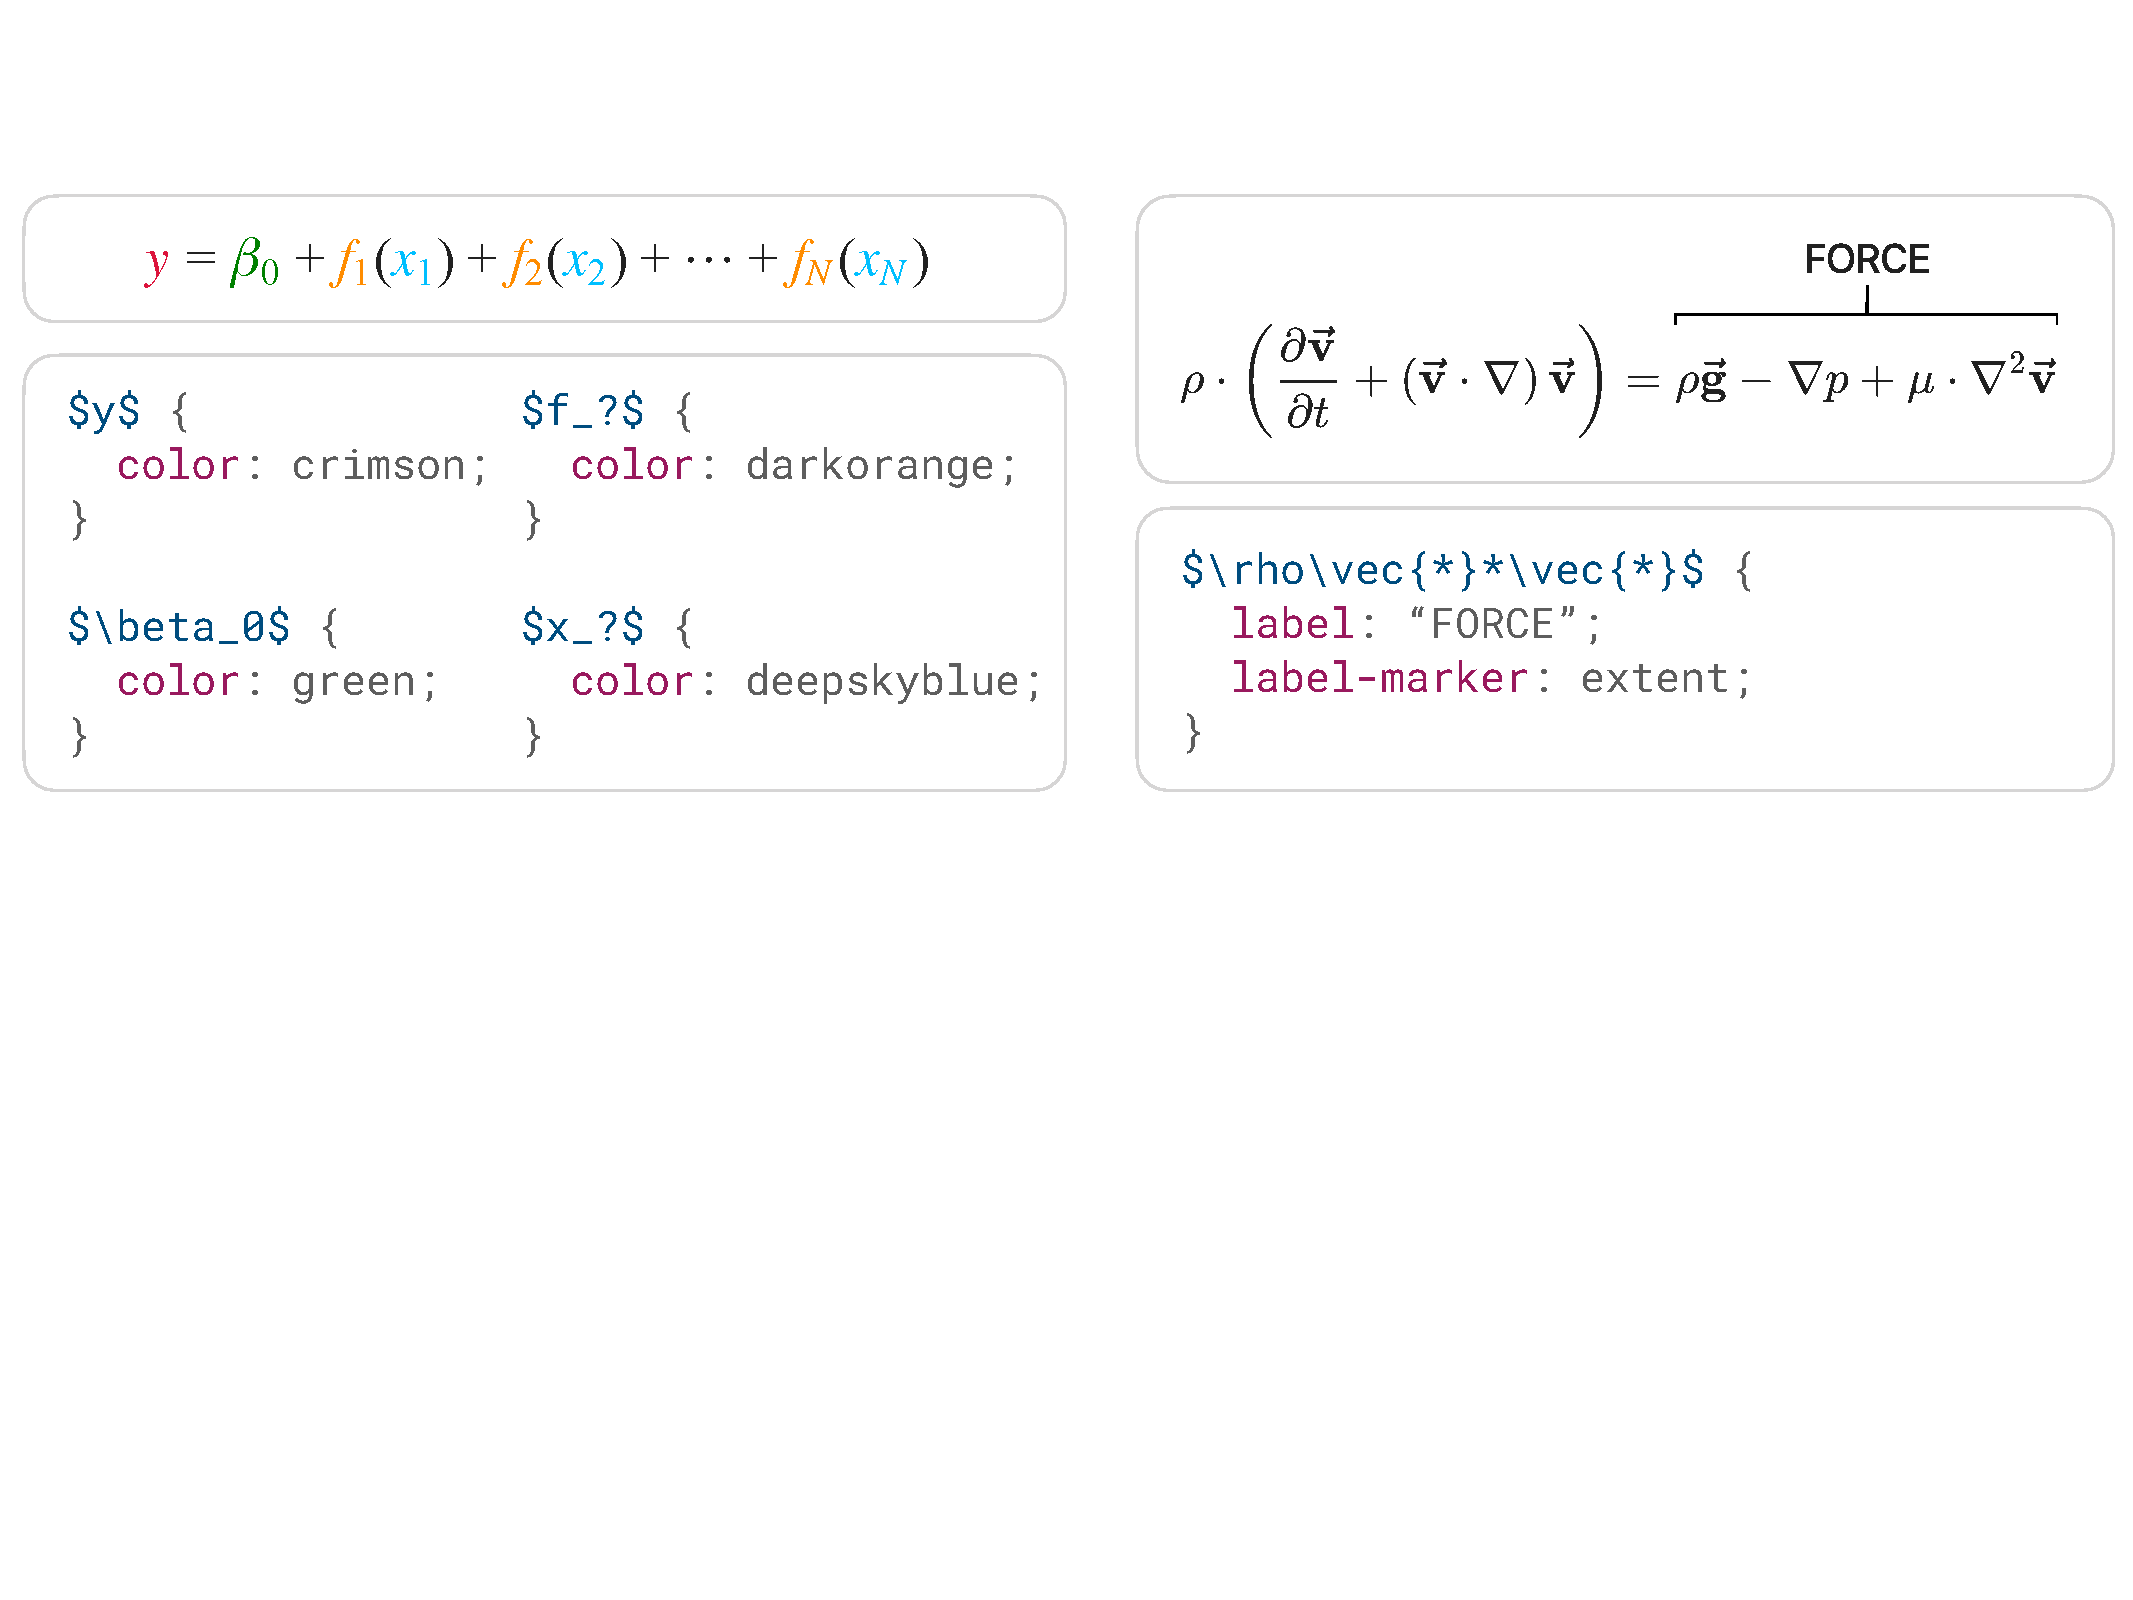
\includegraphics[width=\textwidth]{fig/teaser}
  \vspace{-5ex}
  \caption{Two augmented formulas and their accompanying augmentation specifications written in FFL (``Formula Formatting Language''). \normalfont FFL is designed to be concise, writable, readable, and integrable into web-based document authoring environments. Augmentations are specified using selectors (\textcolor{teasercyan}{dark blue}) that match classes of expressions, and properties (\textcolor{teasermagenta}{magenta}) that apply augmentations like color and labels to formulas. The language can be processed with its live runtime offering rapid feedback to notation authors. The pictured augmentations are adapted from those in documents by \citet{ref:hohman2019gamut} and \citet{ref:murad2020navierstokes}.}
  \vspace{2ex}
  \Description{Two formulas augmented using FFL. Each formula is shown with an FFL style block augmenting it below the formula. The FFL style code consists of selectors and style properties. The first formula is a linear combination formula, where different expressions are colorized; the second formula is a Navier-Stokes equation, augmented with an extent label describing the right side of the formula as describing “FORCE.”}
  \label{fig:teaser}
\end{teaserfigure}

\received[Revised]{29 July 2023}
% \received[revised]{12 March 2009}
% \received[accepted]{5 June 2009}

\maketitle
\ifreview
\raggedbottom
\else
\raggedbottom\pagebreak\flushbottom
\fi
\section{Introduction}

Notation poses a barrier to understanding mathematical ideas. Whether in the physics classroom, data science research papers~\cite{ref:mysore2023how}, or programming documentation~\cite{ref:cai2019software}, readers find important knowledge locked behind the formalisms of formulas and symbols. 
Consider a reader encountering this formula in a research paper \cite{ref:hohman2019gamut}:

% To develop this understanding, learners need to engage with mathematical ideas in the languages that they are expressed. However, when the background of the reader does not match the expectations of the learning material, this could impose a barrier to effective comprehension.

\begin{center}
\vspace{1ex}
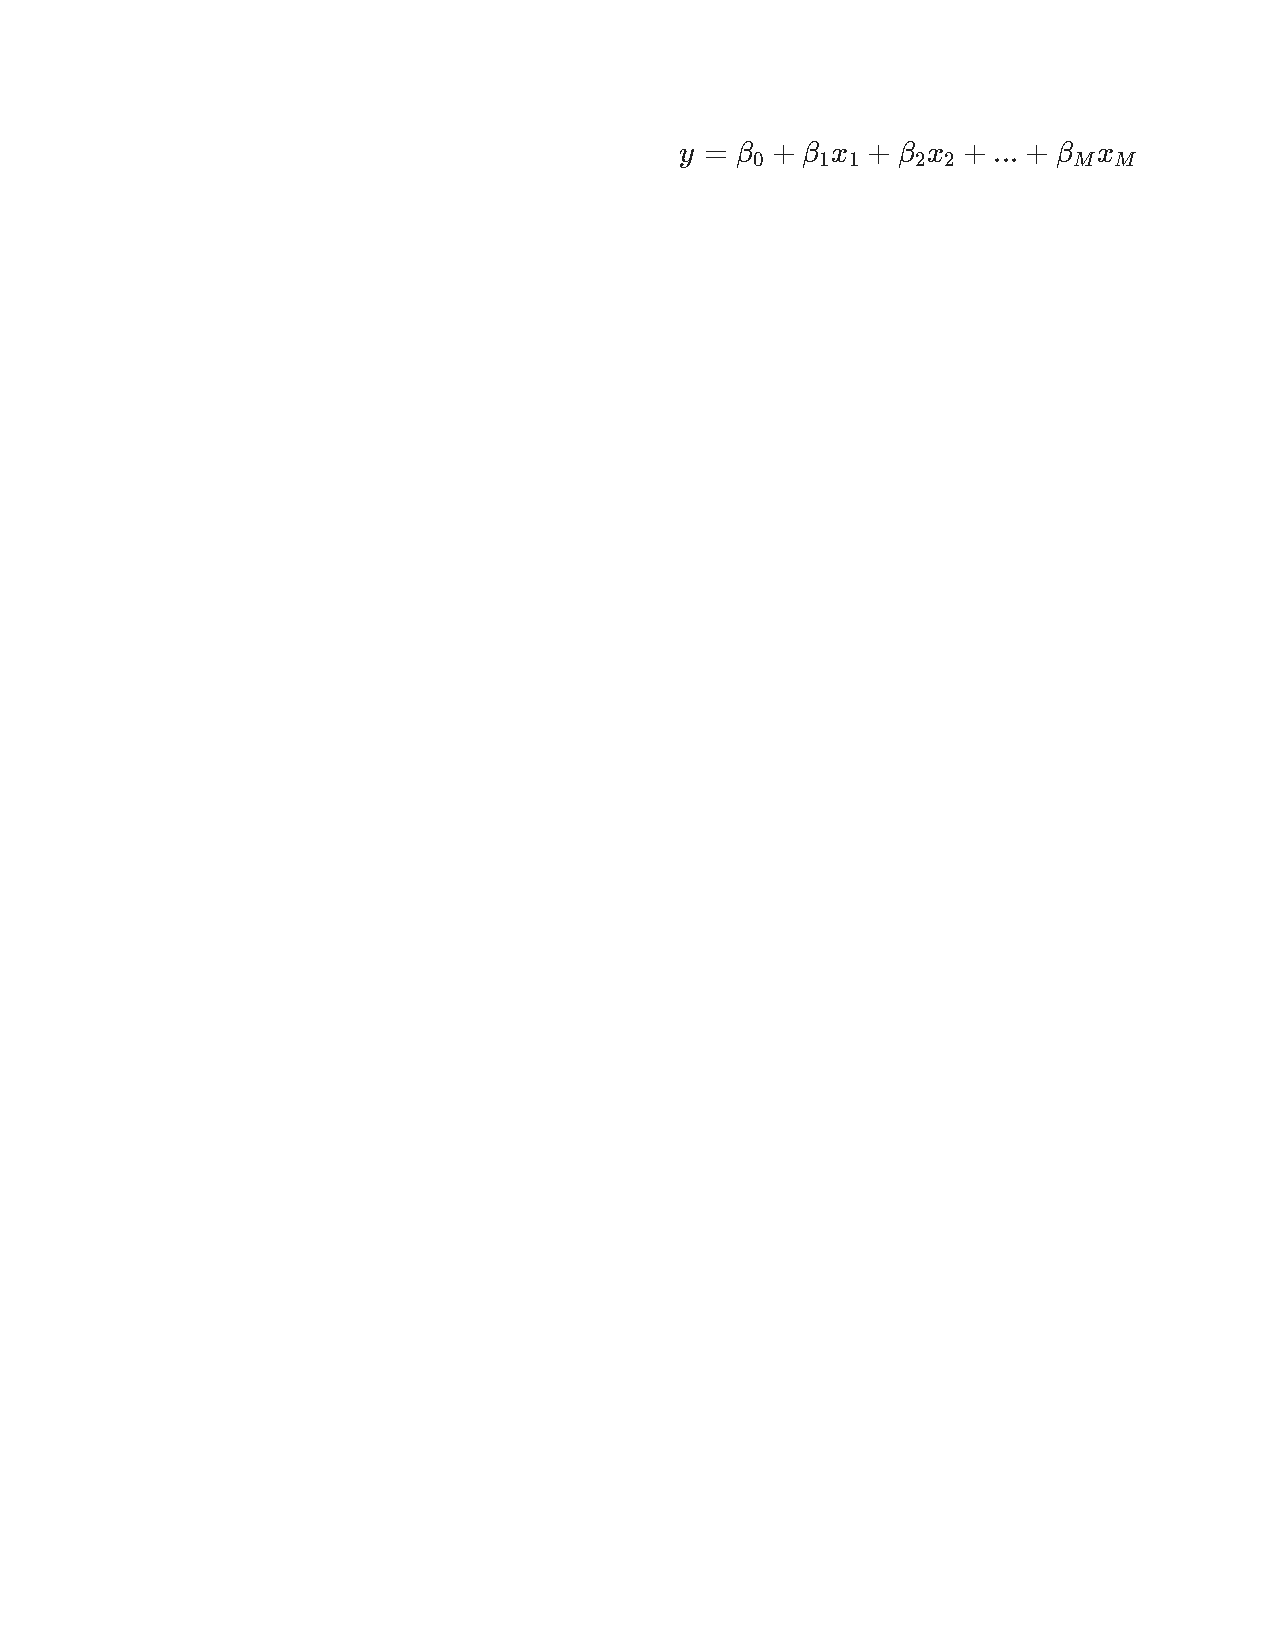
\includegraphics[width=0.62\linewidth]{fig/pre-aug-intro}
\end{center}
\vspace{-0.5ex}

This formula represents a linear regression model. If the reader is not familiar with its idioms, they are likely to find it hard to understand. For instance, what is ``$x$'' and how is it different from ``$\beta$''? $\beta_0$ and $\beta_1$ share a common base---how are they related? What is the intuition of the formula as a whole?

Suppose the formula was instead shown as follows:

% \vspace{-.2ex}
\begin{center}
\vspace{0.5ex}
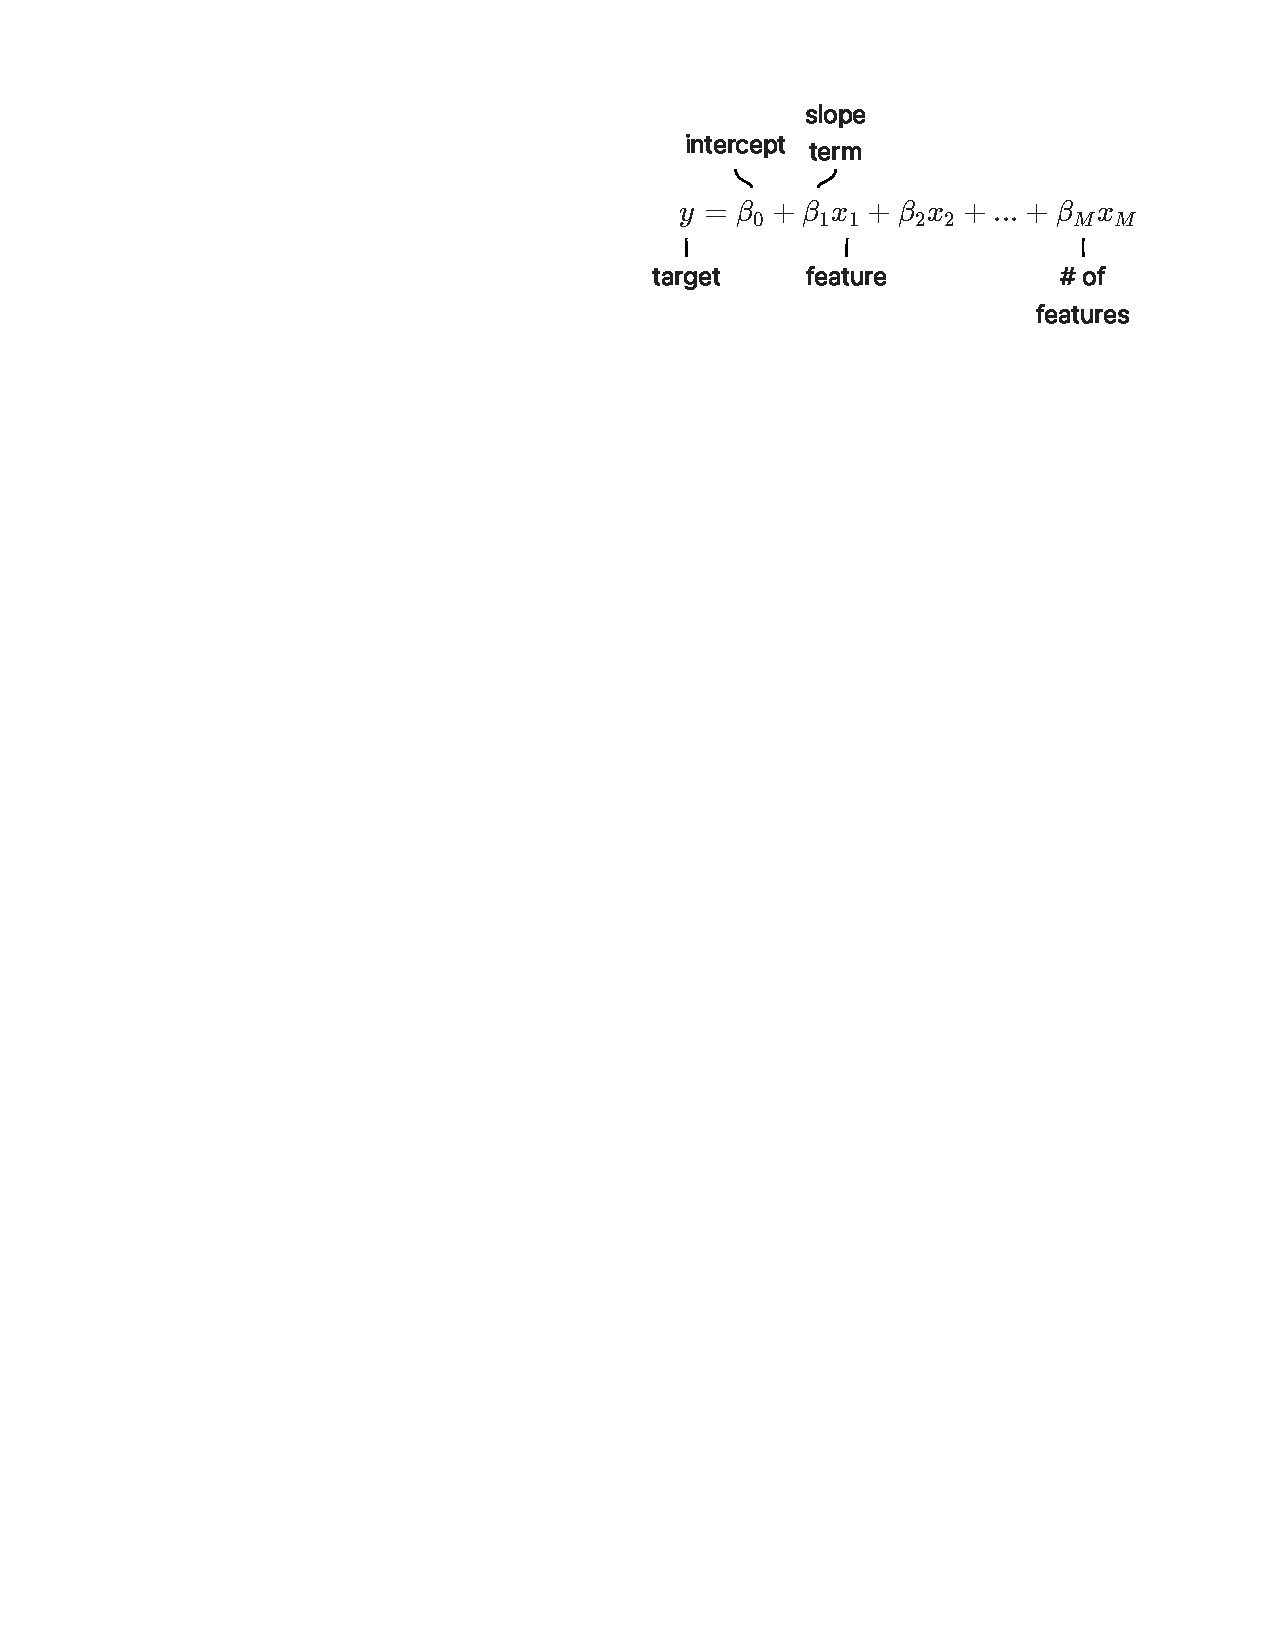
\includegraphics[width=0.65\linewidth]{fig/aug-intro}
\Description{A linear regression formula, augmented with descriptive labels. “y” is labeled “target”; “beta-sub-0” is labeled “intercept”; “beta-sub-1” is labeled “slope term”; “x-sub-1” is labeled “feature”; “beta-sub-M” is labeled “number of features.”}
\vspace{0.5ex}
\end{center}
% \vspace{-.5ex}

This alternative presentation helps a reader to unpack the meaning of a formula. It helps the reader understand the purpose of the formula as predicting a target value from a set of input features. It clarifies that ``$x$'' terms correspond to features, and ``$\beta$'' terms correspond to weights. And it brings the formula into a realm of familiarity by relating ``$\beta_0$'' and ``$\beta_1$'' to the ideas of intercept and slope terms that are taught in algebra class.
Annotated formulas like these help readers grasp their meaning at glance. The annotations' value becomes particularly pronounced when applied to formulas of yet greater complexity and domain specificity.

In this paper, we seek to advance the state of the art in tooling that allows authors to create augmented formulas like these. A recent survey by \citet{ref:head2022math} reveals the challenges present in building effective interactive tooling for this purpose. Conventional formula typesetting tools often make it a ``struggle'' to augment formulas. Formula markup gets too messy, and environments provide insufficient support for experimenting with cross-document formula styling choices.

Our contribution is a reinvention of the process of augmenting formulas in typesetting tools. We envision formula augmentation as a process that involves a crisp markup language and live incremental feedback. We reify this vision in \emph{FFL}, or ``Formula Formatting Language,'' a markup language for formula augmentation. FFL is targeted for web-based math document authoring. Its key innovations are a design that splits augmentation markup from formula markup, a CSS-inspired familiar syntax, support for cross-document styling, and an implementation that permits live feedback.

% In this paper, we envision an improved authoring experience where users are enabled to separate their augmentation and formula specifications, apply augmentations to multiple expressions simultaneously, and rapidly experiment with alternative augmentations. The result is a language called \emph{FFL}, or ``Formula Formatting Language,'' and an accompanying live runtime.

% Here, a reader can easily gauge what each variable stands for, track which terms in the equation are related, and understand their usage in the equation.

% While augmentations facilitate better comprehension, the tools that authors use to present formulas often introduce friction in doing so. In a recent survey, \citet{ref:head2022math} describe that authors find themselves using tools that involve clunky markup languages, ugly defaults, and tedious graphic editing.

% One class of tools that poses friction is markup languages for typesetting formulas. Today, TeX~\cite{ref:knuth1986tex} is perhaps the most widely-used markup language for expressing formulas. Yet, augmenting formulas with a TeX tool requires injecting augmentation code (e.g., color and label macros) into the underlying formula. This results in an experience described a ``struggle''~\cite{ref:head2022math} as markup becomes difficult to read and efficiently edit. Furthermore, unless an author has been disciplined about defining expressions using macros, it can be time-consuming to alter style choices across formulas.

We assess FFL's impact on the authoring experience in a controlled usability study where 28 participants used FFL and \zed{a} LaTeX baseline.
\zed{In complex editing tasks, FFL increased efficiency and self-reported ease, and led to more readable augmentation code versus the baseline. For tasks involving writing simple augmentations from scratch, FFL and LaTeX showed no significant difference.}
% \zed{FFL increased efficiency, self-reported ease, and led to more readable augmentation code when participants performed complex editing tasks, and yielded no observed performance difference for simpler authoring tasks.}
Reviewing the evidence in the framework of the cognitive dimensions of notation~\cite{ref:blackwell2003notational}, our study suggests FFL reduces viscosity, hard mental operations, and error proneness, while benefiting from closeness of mapping and progressive evaluation. These results suggest that FFL-like languages could make the formula augmentation task better supported in contemporary authoring tools.

In summary, this paper contributes:
\begin{itemize}
% \vspace{-1ex}
\item The design of \emph{FFL}, a markup language for augmenting formulas, designed for readability and efficiency,
\item A runtime supporting live application of augmentations to formulas in web-based authoring environments, and
\item Evidence from a usability study that FFL leads to faster and easier edits to augmentation markup and results in more readable markup.
\end{itemize}

\section{Background and Related Work}

% SHORTENING OPPORTUNITY: maybe replace the following with:
% SHORTER VERSION: In this section, we discuss why authors might wish to augment notation and then situate our system amidst related work.
In this section, we discuss why authors might wish to augment notation and then situate our work relative to prior tools for authoring and augmenting formulas.

% In this section, we review why an author might wish to augment math notation. Then, we review prior tools that support augmentation of notation, crystallizing the purpose of FFL as providing a lightweight markup language for use in web authoring contexts. We also relate FFL to recent HCI systems that provide similar affordance for different kinds of documents.

\subsection{Notation and augmentation}

Math notation is difficult to read. It has been described as a language of its own, requiring practice to understand~\cite{ref:adams2003reading}. Over time, the human perceptual system can become trained to recognize structures in formulas~\cite{ref:marghetis2016mastering}. Readers learn idioms in formulas through repeated exposure, such that experts can spot structures in formulas novices miss~\cite{ref:shepherd2014reading}. For novices, notation poses a barrier to understanding mathematical texts and is often cited as a challenge in self-teaching machine learning~\cite{ref:cai2019software} and reading research papers~\cite{ref:mysore2023how}.

Subtle changes to the presentation of notation can affect its readability. For instance, coloring and annotating formulas can reduce cognitive load in solving algebra problems~\cite{ref:yung2015effects}. Readers can be aided in understanding operator precedence by altering which letters are used for variables and spacing between variables~\cite{ref:goldstone2017adapting,ref:harrison2020spacing}. The design space for augmented notation is large. \citet{ref:dragunov2003designing} propose augmenting formulas with symbols definitions, annotations that show how variables are manipulated across stages of derivation, and controls that adjust the level of detail in a derivation. \citet{ref:head2022math} and Hohman et al.~\cite{ref:hohman2020awesome} expand this design space, with the former describing 16 classes of augmentations.
In this paper, we explore how authoring environments could be extended to equip authors with tools to perform common some of the most common kinds of augmentations.

\subsection{Tools for augmenting notation}

% Authors have at their disposal many tools for augmenting notation, including markup languages for typesetting formulas, graphical editors, and sketching tools. A recent interview study by \citet{ref:head2022math} suggests that authors using these tools encounter friction of various kinds. This paper is particularly focused on improving the experience of reading and writing markup code, experimenting with cross-document styling rules, and baking good visual design into augmentations.

\paragraph{Markup languages}

One of the most common kinds of tools for writing and augmenting notation is the markup language. Markup languages, like TeX~\cite{ref:knuth1986tex}, allow authors to write formulas in plain text and render them as cleanly typeset formulas. Some such tools provide support for augmentation. LaTeX~\cite{tool:latex}, for instance, supports the addition of color with the \texttt{color}~\cite{tool:carlisle1997color} package, and labels with macros from the \texttt{mathtools}~\cite{tool:madsen2014mathtools} and \texttt{annotate-equations} ~\cite{tool:annotateequations} packages. Recent research suggests that these tools could benefit from cleaner markup design, better defaults, and better support for cross-document style changes~\cite{ref:head2022math}.

The popularity of TeX as a language for formula typesetting has led to web-based TeX formula typesetters. One such tool is KaTeX~\cite{tool:katex}. The context of the web provides new opportunities for augmentation. KaTeX offers authors the \texttt{\textbackslash{}htmlClass} for assigning HTML classes to arbitrary expressions. CSS can then be used to apply styles to those expressions. Our goal with FFL was to support augmentation of TeX formulas in web-based authoring environments using a language similar to CSS.

Notation augmentation is a feature of several recent markup languages for math and science communication. Nota~\cite{ref:crichton2021new} and Heartdown~\cite{ref:li2022heartdown} let authors specify definitions of symbols, revealing symbol definitions in the margins of selected formulas when clicked upon. Curvenote's editor API~\cite{tool:curvenote} provides support for parametric LaTeX formulas, where numeric values can be substituted into formulas as users interact with widgets. \emph{manim}~\cite{tool:manim} supports the creation of animations of math formulas with step-by-step builds and incremental annotation. We share motivation with these projects, aiming to create an extensible augmentation language and runtime for static math texts~\cite{ref:head2022math}.

Why focus on augmentation in markup editors rather than other sorts of document editors? Markup, and in particular TeX, is used pervasively within the sciences and academia.
% SHORTENING OPPORTUNITY
% SHORTER VERSION: It is a preferred tool for disseminating and archiving mathematical ideas~\cite{ref:misfeldt2011computers}.
It is a preferred tool for writing math notation not necessarily for sketching out ideas, but rather for disseminating or archiving them~\cite{ref:misfeldt2011computers}.
One study suggests writers can enter notation-dense passages more efficiently with TeX than with structured editors~\cite{ref:knauff2014efficiency}. TeX is used widely enough that WYSIWYG editors like Word have incorporated it as a language for formula input~\cite{ref:matthews2019craft}. We see the development of effective markup-based augmentation tools as a natural springboard for efforts to develop better augmentation tools generally.

% \textit{MathML}~\cite{tool:mathml} is a dialect of XML that allows authors to write formulas using a structured markup language; expressions in the rendered formulas can be styled using CSS. Our initial aim with FFL was to leverage the familiar language of CSS for augmentation in conjunction with the familiar method of writing formulas using TeX, in a way that supports efficient selection of expressions separate from the formula markup.

\paragraph{Structured editors}

WYSIWYG document editors like Word~\cite{tool:wordformulaeditor} sometimes provide structured formula editors. These editors can be used to augment formulas by selecting labels from menus, or by applying their tools for formatting text. Toolkits like MathType make such functionality available as a plugin to other editing applications~\cite{ref:topping1999using}. One advantage of these tools is that their WYSIWYG design makes augmentation affordances easier to discover.
% ; we discuss the ability to combine structured editors with languages like FFL in the discussion.

\paragraph{Vector graphics editors}

Formulas can be augmented using vector-based graphics editing software; Head et al.'s study describe Google Slides~\cite{tool:googleslides}, Inkscape~\cite{tool:inkscape}, Mathcha~\cite{tool:mathcha}, and PowerPoint~\cite{tool:powerpoint} as several tools that authors are already using. Some of these tools require authors to render formulas outside of the environment (e.g., with CodeCogs~\cite{tool:codecogs}) and import the render as a bitmap or vector graphics into the editor. These tools are often both familiar to authors and flexible---authors can add augmentations using the full complement of text formatting and shapes the tools provide.  FFL and vector graphics editors occupy two complementary areas of the augmentation design space, with FFL focusing on supporting typesetting experience and transferable styles, and vector graphics editors offering flexible augmentation through direct manipulation.

% \andrew{Can we add in e-Proofs~\cite{ref:alcock2011eproofs} here? I can't remember what its authoring environment looks like.}

\paragraph{Sketch and gesture}
Formulas can also be written and augmented as sketches~\cite{ref:laviola2006mathpad2,ref:zeleznik2010hands,ref:leitner2010nice,ref:saquib2021constructing}. In sketching tools, augmentations are naturally supported when authors are given the ability to change ink color and draw free-form shapes. Some sketching tools support unique augmentations, like linking expressions to sketched physical objects~\cite{ref:laviola2006mathpad2,ref:saquib2021constructing}, or manipulating expressions with gestures~\cite{ref:zeleznik2010hands,ref:weitnauer2016graspable,ref:mendes2014structure}. Some of these affordances could be adapted as advanced augmentations for languages like FFL in the future.

\paragraph{Automation}
As text understanding techniques improve, it may be possible to automatically augment notation. Myriad projects have explored the ability to detect the positions of symbols~\cite{ref:head2021augmenting} and parse formulas ~\cite{ref:anthony2005evaluation,ref:ma2021latexify} from arbitrary input documents. Should it become possible to reliably detect expressions and their meaning automatically, augmentations could be added to documents with reduced input from authors.

\subsection{Tools for augmenting texts}
Our work draws inspiration from HCI research that develops powerful text authoring affordances generally.

\paragraph{Repetitive text editing}
One challenge in editing longer texts is making repetitive edits when revising repeated phrases and ideas. HCI research has proposed numerous techniques to do so, including linked editing~\cite{ref:toomim2004managing}, detection and propagation of edits~\cite{ref:miltner2019fly,ref:ni2021recode}, and editable macros~\cite{ref:han2020textlets}. FFL's approach is to allow authors to use CSS-style selectors to indicate which expressions to augment. These selectors allow authors to apply and edit augmentations for many related expressions at once.

\paragraph{Diagrams}
One of the facilities of FFL is to support the creation of simple formula diagrams where descriptive labels are linked to expressions. Researchers have developed powerful domain-specific languages supporting for diagramming like Penrose~\cite{ref:ye2020penrose} and Bluefish~\cite{ref:pollock2022bluefish}. In comparison to these prior toolkits, the aim of FFL's labeling system is to support ease and conciseness in supporting a common, simple sort of labeling, among other augmentations.

\paragraph{Live feedback}
FFL supports third-level or ``edit-triggered'' liveness, according to Tanimoto's taxonomy of liveness~\cite{ref:tanimoto1990viva}. Liveness has been a central feature of dozens of research systems~\cite{ref:rein2018exploratory}. Its use in LaTeX tooling (e.g.,~\cite{ref:gobert2022ilatex,ref:dragicevic2011gliimpse}) may arise from the fact that LaTeX documents require time-consuming compilation to view the effect of a change. FFL incorporates liveness to equip authors with more rapid feedback as they are experimenting with augmentations.

% As with any user interface, a markup language that offers rapid feedback reduces the time it takes an author to understand the effects of their actions. FFL was designed and implemented to allow for live re-rendering, in contrast to typical LaTeX tools that require recompilation. The difficulty of mapping between one's LaTeX and the resulting rendered document has previously led to the design of widgets that provide context-local rendering of parts of LaTeX documents~\cite{ref:gobert2022ilatex}, and programming environments that use animation to show how tokens in LaTeX correspond to tokens in the rendered document~\cite{ref:dragicevic2011gliimpse}. FFL provides live feedback specifically on augmentations; to enable this in a web authoring environment required careful integration with the KaTeX formula typesetter. 

% Old stuff

% This research is motivated by a recently-conducted needs assessment~\cite{ref:head2022math}. The challenges from that paper that this one aims to address are clunky markup, and cross-document changes.

% \andrew{Give a brief overview of research that suggests that augmentations to formulas might influence how they are read. Refer to Ottmar paper that describes how our brain is rewired through repeated exposure to be able to process formulas.}

% When considering the space of tools for augmenting math formulas, tools are of several kinds. The first is WYSIWYG formula editing tools, like the built-in formula editor in Microsoft Word. The second are general purpose vector graphics editing tools, like PowerPoint or InkScape---formulas can be rendered as bitmaps or vector graphics, and then edited as basic vector graphics in these programs by colorizing expressions, adding labels, and so on. A third kind are typesetting tools, like LaTeX and its accompanying packages for colorizing and labeling formulas~\cite{tool:annotateequations}.

% There are also sketch- and gesture-based formula editors. This includes MathDeck, Saquib et al.'s project, Graspable Math, and Hands-on Math. These projects suggest affordances for creating and manipulating formulas that are more direct than writing in typesetting languages. Our project assumes that formulas are written using a typesetting language like LaTeX.

% Some LaTeX editors make the authoring of formulas easier. Examples include i-LaTeX, the Daum Equation Editor, and other projects.

% There are related projects on creating diagrams automatically, including 

% Other projects provide similar affordances for texts and visualizations generally. Textlets supports making cross-cutting edits to terms and phrases in a document. Potluck and Tangle.js, and Kay et al.'s multiverse analysis enliven texts in another way, allowing readers to change values in a text, and see their effect to downstream computations (e.g., test statistics, quantities in a recipe, etc.) computed. Parametric Press provides another example.

% \andrew{And then an even older version of the related work has been commented out below}
% There has long been need for richer formats that facilitate readers to better
% comprehend math documents as it is often not straightforward with sometimes large
% and/or local nomenclature of notations that might be visually busy or difficult to
% navigate \cite{MathComm}. And despite the advancement of digital
% typesetting and the variety of document setting tools that allow augmentations to math notations,
% there remains pain points and barriers to quick design and application of
% these desired augmentations \cite{MAug} in these math documents.

% There have been many attempts in creating tools to make powerful math augmentations
% more accessible and easier to create. \textit{i-LaTeX}\cite{iLaTeX} approaches this by
% creating ``transitional representations'' that maintains the power of code fragments
% while taking lessons in direct manipulation from WYSIWYG interfaces. There are also
% \textit{Penrose}\cite{Penrose}, \textit{Bluefish}\cite{Bluefish} who lean into the
% code/language-based approach as we do, but generally define their grammar from the ground up.
% We also find more powerful domain-specific tools already in production use, such as
% \textit{Manim}\cite{manim}, an animation engine by the immensely popular math educational video creator
% \textit{3Blue1Brown}, which has since been forked and maintained by the community.

% These tools create incredible opportunities to created enhanced presentation of
% math documents, but some incur a significant learning curve while others are not
% as general-purpose as we would like.



% Another version of the outline appears below...
% Notation can be difficult to understand.
% \cite{ref:cai2019software}
% \cite{ref:adams2003reading}
% (It is hard to read in papers)
% \cite{ref:mysore2023how}
% (Experts appear to parse formulas differently than less experienced readers).
% \cite{ref:shepherd2014reading}
% (Learning algebra retrains the visual system to parse structures).
% \cite{ref:marghetis2016mastering}
% Practices have emerged for augmenting notation.
% \cite{ref:head2022math}
% \cite{ref:3Blue1Brown}
% \cite{ref:hohman2020awesome}
% \cite{ref:dragunov2003designing}
% Such practices may be able to help readers.
% \cite{ref:harrison2020spacing}
% \cite{ref:goldstone2017adapting}
% \cite{ref:yung2015effects}
% But these tools remain difficult to use.
% \cite{ref:head2022math}

% Mathematicians write notation. They often do so using typesetting tools. While there are of course advantages to writing by hand, typesetting tools remain in widespread use.
% % Mathematicians write notation. They often do so using typesetting tools.
% \cite{ref:misfeldt2011computers}
% \cite{ref:knuth1986tex}
% % While there are of course advantages to writing by hand or using WYSIWYG editors...
% % (Writing by hand often outperforms digital tools, even if not LaTeX...)
% \cite{ref:quinby2020effects}
% \cite{ref:anthony2005evaluation}
% % (Word is usable for authoring formulas)
% \cite{ref:loch2015master}
% % One measure suggests that typesetting led participants to write formulas more quickly
% \cite{ref:knauff2014efficiency}
% % Typesetting tools remain in widespread use.
% \cite{ref:matthews2019craft}

% \paragraph{Markup languages}
% First, there are facilities within markup languages (LaTeX, KaTeX's extensions, MathML, etc.)
% \cite{tool:latex}
% \cite{tool:carlisle1997color}
% \cite{tool:madsen2014mathtools}
% \cite{tool:annotateequations}
% \cite{tool:katex}
% \cite{tool:mathml}
% \cite{ref:igalia2023igalia}
% There are also other assistive tools for authoring LaTeX. One particular set of technologies helps a reader track correspondences between tokens in the LaTeX (in either prose or in equations) and corresponding tokens in the compiled PDF.
% \cite{ref:gobert2022ilatex}
% \cite{ref:dragicevic2011gliimpse}
% There are also new markup languages emerging that support augmented math.
% % (I need better differentiation from Nota and Curvenote, and to express why we did not compare to them).
% \cite{ref:crichton2021new}
% \cite{ref:li2022heartdown}
% \cite{tool:curvenote}
% % Nota (macros for coupled underlining of text and expressions, and facilities for defining definitions)
% % Heartdown (provides pointers from symbol definitions to their use), and links between notation and generated visualizations.
% % Curvenote (provides macro-based grammar for colorizing, and simple utilties for symbold efinitions).
% % manim.
% This research was motivated by a feeling that new syntaxes were needed that could provide both a low threshold and eventually a high ceiling~\cite{ref:myers2000past}, along with simple expression of common augmentations. For instance, we believe it should be easy to colorize formulas, and to define always-on augmentation; these require a different way of thinking about processing the markup. Furthermore, we envision leveraging authors' existing knowledge of languages like CSS to support their writing.
% \andrew{One of the ways in which we can differentiate is in stating that we are trying to conduct user-centered research and evaluations to assess the usability of these markup languages (I think a lot of this prior work has not done so, and I think it is really important).}

% \paragraph{Structured editors}
% Second, they could be added with WYSIWYG editors with menus for selecting symbols and structures.
% \cite{ref:topping1999using}
% \cite{tool:wordformulaeditor}

% \paragraph{Vector graphics editors}
% Third, they can add annotations through vector graphics editing software.
% \cite{tool:googleslides}
% \cite{tool:inkscape}
% \cite{tool:mathcha}
% \cite{tool:powerpoint}
% \cite{tool:keynote}
% (And through slides-based editing applications)
% \cite{ref:alcock2011eproofs}
% Some of these tools (Mathcha, Keynote) allow writing LaTeX for formulas, and then adding annotations on top of them with typical drawing tools. To our knowledge, these tools do not support the ability to transform formulas into vector graphics. Authors have, in the past, converted them to vector graphics themselves using tools like CodeCogs.
% \cite{tool:codecogs}

% \paragraph{Sketching tools}
% Fourth, people can sketch formulas in more general-purpose drawing applications.
% \cite{ref:laviola2006mathpad2}
% \cite{ref:zeleznik2010hands}
% \cite{ref:leitner2010nice}
% These formulas can be linked to complementary expressions and sketches.
% \cite{ref:laviola2006mathpad2}
% \cite{ref:saquib2021constructing}
% They can also interact with gestures.
% \cite{ref:zeleznik2010hands}
% \cite{ref:weitnauer2016graspable}
% \cite{ref:mendes2014structure}
% (Visual processing of formulas is a technique that has been around for some time)
% \cite{ref:ma2021latexify}

% \paragraph{Automation}
% Finally, augmentations can be produced automatically.
% \cite{ref:head2021augmenting}

% \subsection{Tools for augmenting texts}

% \paragraph{Repetitive text editing}.
% LaTeX provides a macro feature.
% \cite{ref:toomim2004managing}
% For instance, Textlets supports more rapid iteration around terms used in a text.
% \cite{ref:han2020textlets}
% \cite{ref:miltner2019fly}
% \cite{ref:ni2021recode}
% We opt for the CSS approach of defining "selectors"; given that our hope is to preserve the original formula in the original markup without fragmenting it, this format allows us to separate out the style specification from the underlying formula specification.

% \paragraph{Diagramming}.
% We draw inspiration from a few directions of research in the design of our toolkit.
% First are tools that support diagramming.
% We are interested in developing lightweight languages (like BlueFish or ChartAccent) for formulas.
% Our comparisons in this paper are to prior typesetting tools. We envision that the development of grammars that work well as languages could serve as a good foundation for making augmentations in the other kinds of tools.
% \cite{ref:ye2020penrose}
% \cite{ref:pollock2022bluefish}
% \cite{ref:ge2020canis}
% % D3-annotation
% We are interested in separating out style code and substance code (like Penrose).

% \paragraph{Making texts interactive}.
% \cite{tool:victortangle}
% \cite{ref:litt2022potluck}
% \cite{ref:dragicevic2019increasing}
% \cite{ref:conlen2018idyll}

% \andrew{One of the ways in which we can differentiate is in stating that we are trying to conduct user-centered research and evaluations to assess the usability of these markup languages (I think a lot of this prior work has not done so, and I think it is really important).}
\section{Demo}\label{Demo}

FFL is designed to help authors augment formulas with a lightweight syntax and live feedback. Here, we illustrate the envisioned user experience of FFL with a scenario.

Imagine Auggie, a researcher writing \zed{an article in a web-based scientific authoring environment, where text is written in Markdown, HTML, or an HTML-compatible dialect.} They are writing a passage where they introduce the idea of linear regression.\footnotemark\ They wish to help readers understand the gist of this formula, despite the dense appearance of the formula and the accompanying prose: \footnotetext{This example is adapted from an excerpt from \citet{ref:hohman2019gamut}.}\\[1ex]
\ifreview
\else
\centerline{\vspace{3ex}\textcolor{gray}{\textit{(continued on next page)}}}
\vfill\pagebreak
\fi
\aptLtoX[graphic=no,type=html]{\centerline{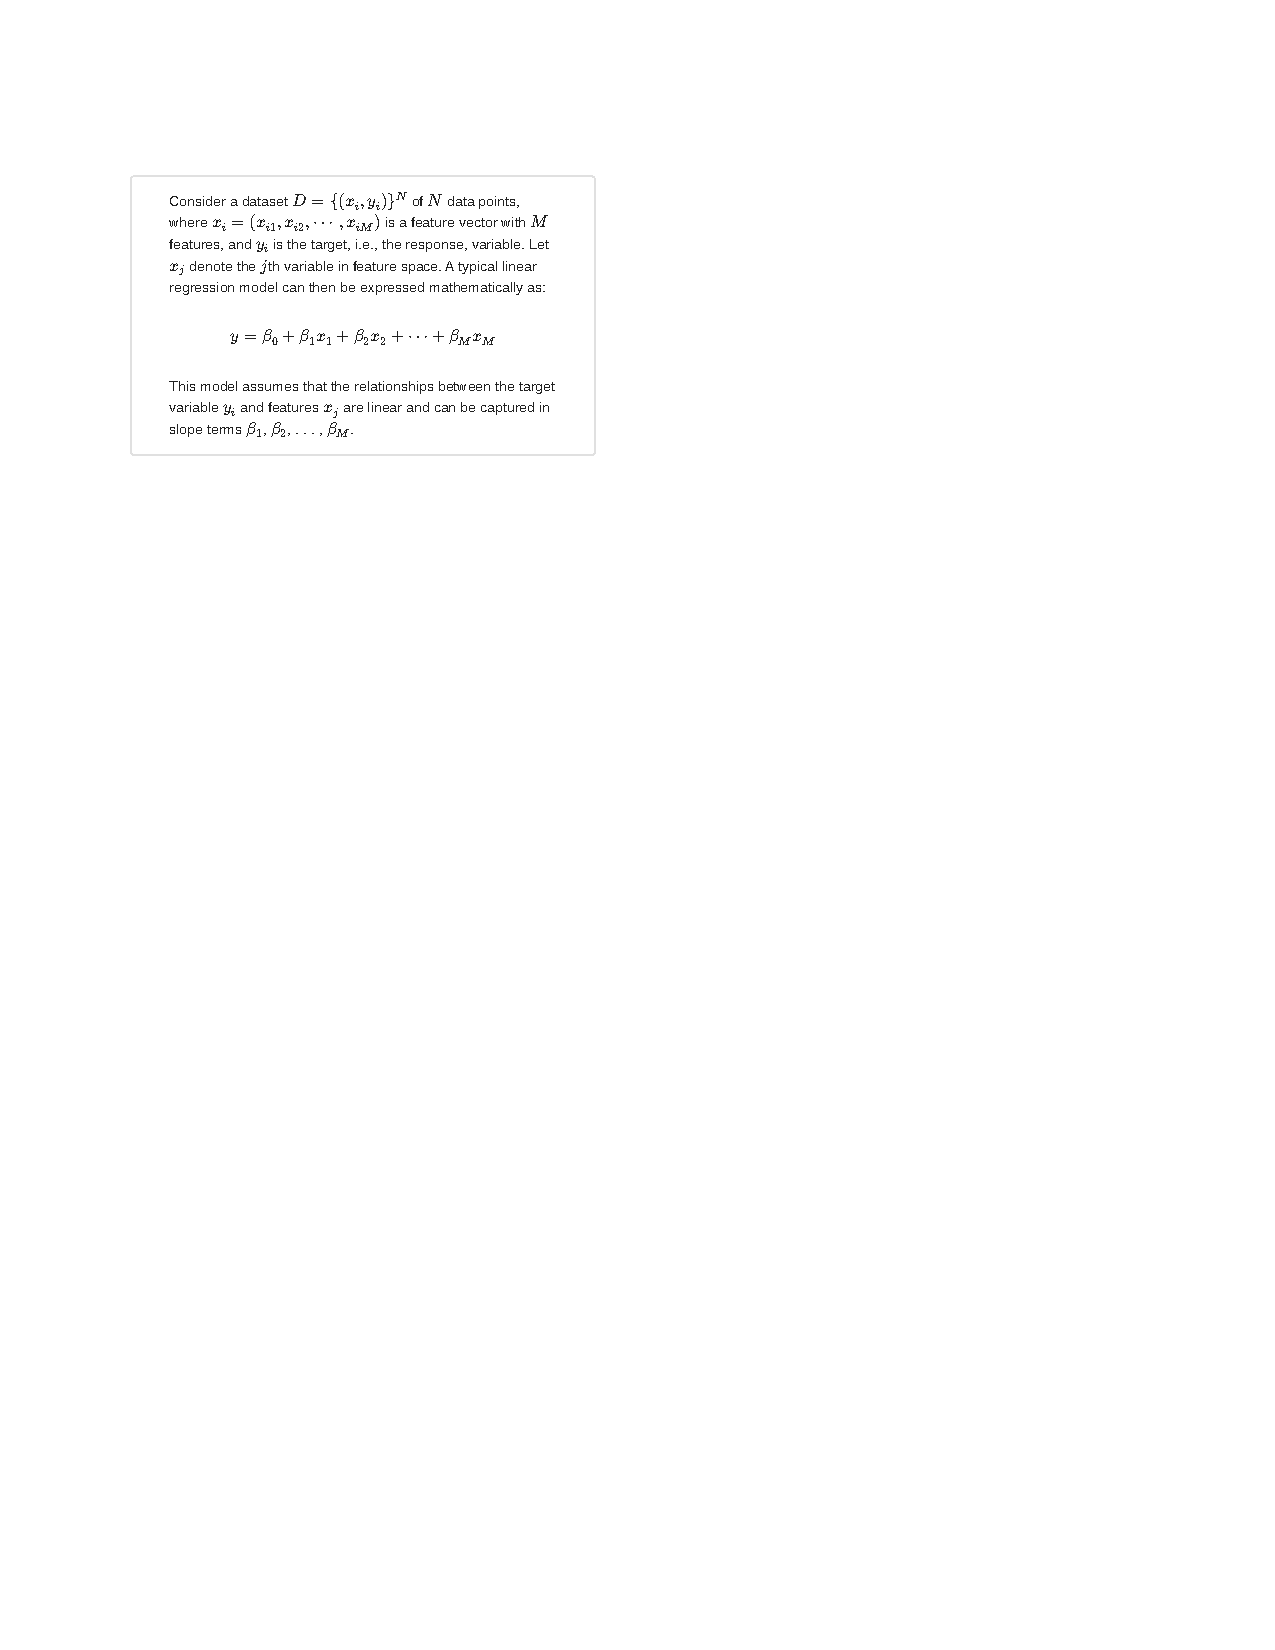
\includegraphics[width=1.02\linewidth]{fig/P4-1.pdf}} }{ \demofig{1}
\Description{An excerpt from a math text that explains a formula for linear regression. The excerpt contains two inline formulas within the text, one block formula, and half a dozen references to individual symbols.} } 


Auggie desires to augment the formula using colors and labels to expose the formula's meaning. Their editor has been extended with support for FFL, which allows them to experiment with these augmentations. Auggie first explores how they could use of color to help readers correlate expressions in the formulas with their descriptions in the text.

To start, Auggie colors the target variable $y$. To do this, they write the following FFL selector and style in a text editor adjacent to their document markup. This helps ensure that the augmentation markup does not clutter the formula or document markup. \\[1ex]
\aptLtoX[graphic=no,type=html]{\centerline{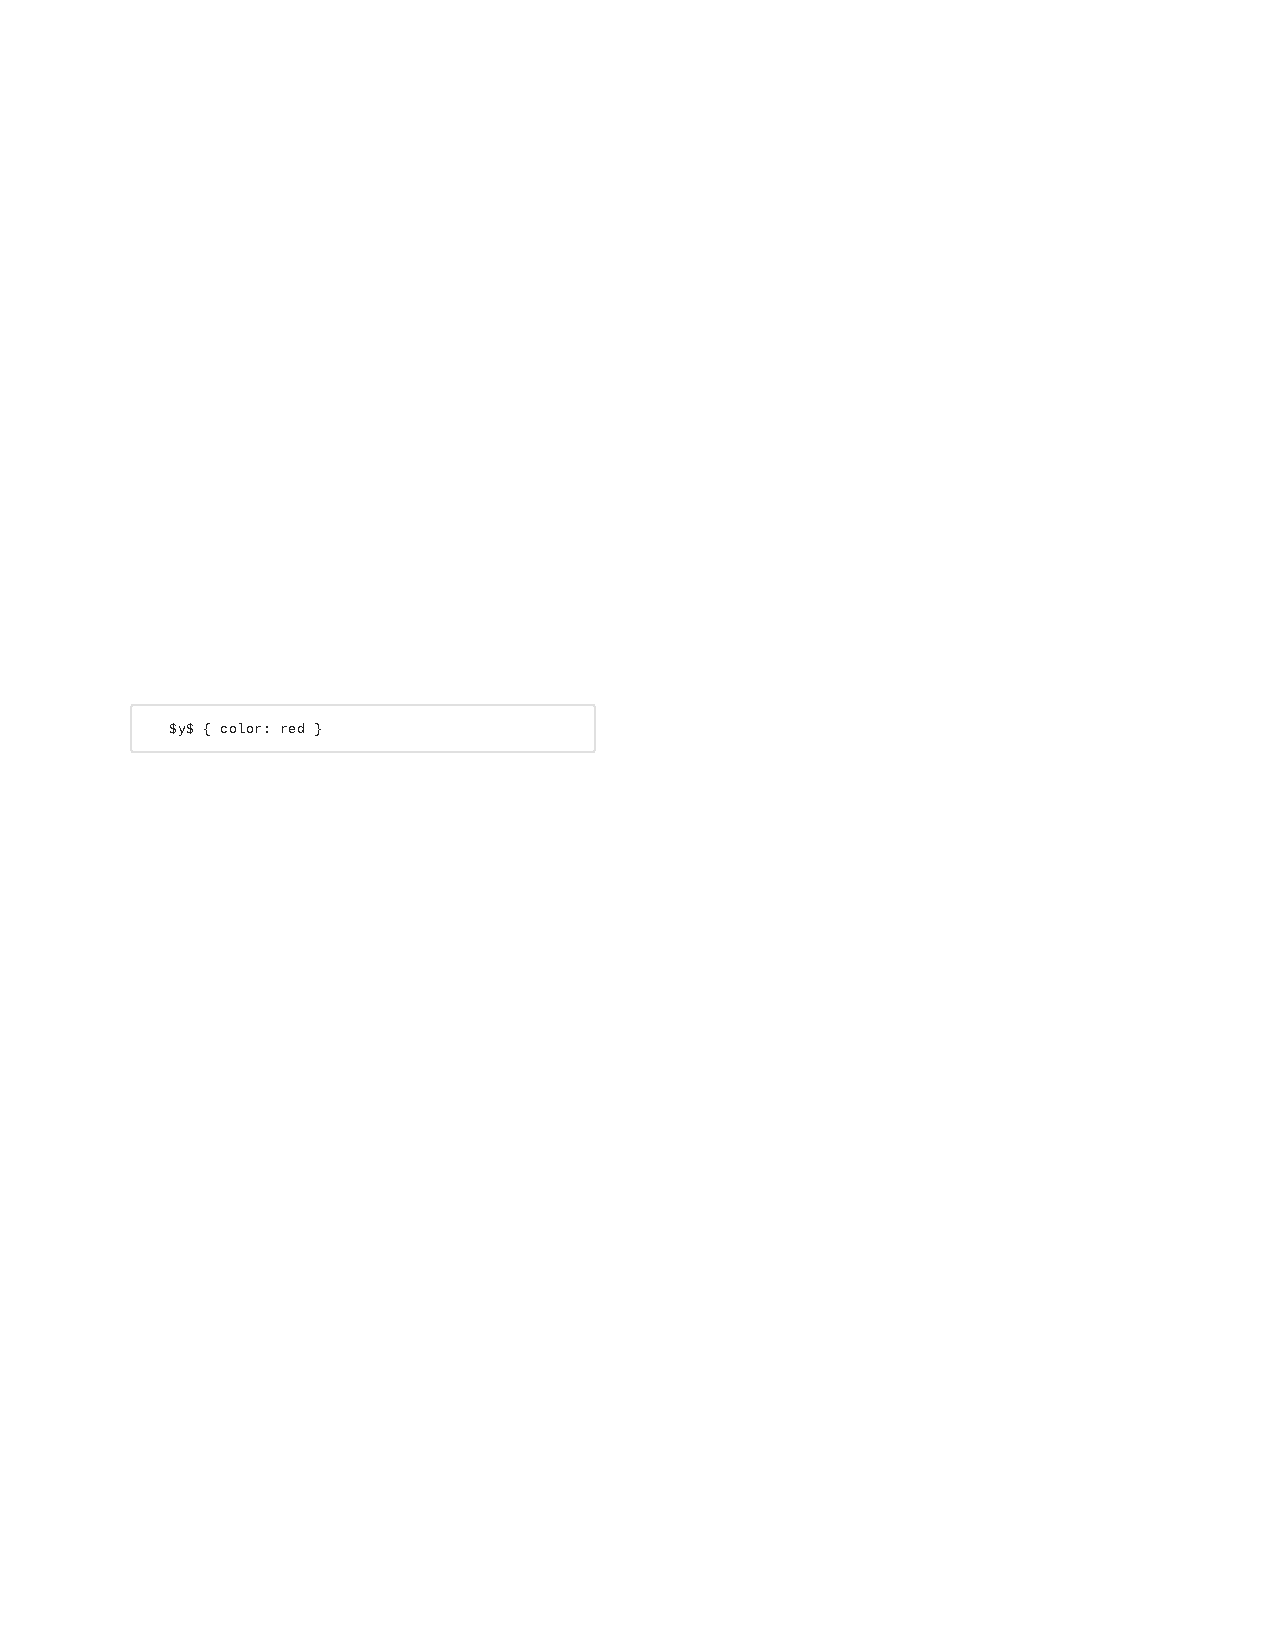
\includegraphics[width=1.02\linewidth]{fig/P4-2.pdf}} }{ \demofig{2}\Description{An FFL augmentation specification, consisting of the selector “$y$” and a declaration to color the matching expressions red.}}  

This markup represents a request to find all instances of symbols described by the LaTeX literal ``\$\texttt{y}\$'' and color them red. The effect is instantaneous: as soon as Auggie finishes typing ``\texttt{red},'' the symbol $y$ is colored red everywhere it appears in the document: \\[1ex]
\aptLtoX[graphic=no,type=html]{ \centerline{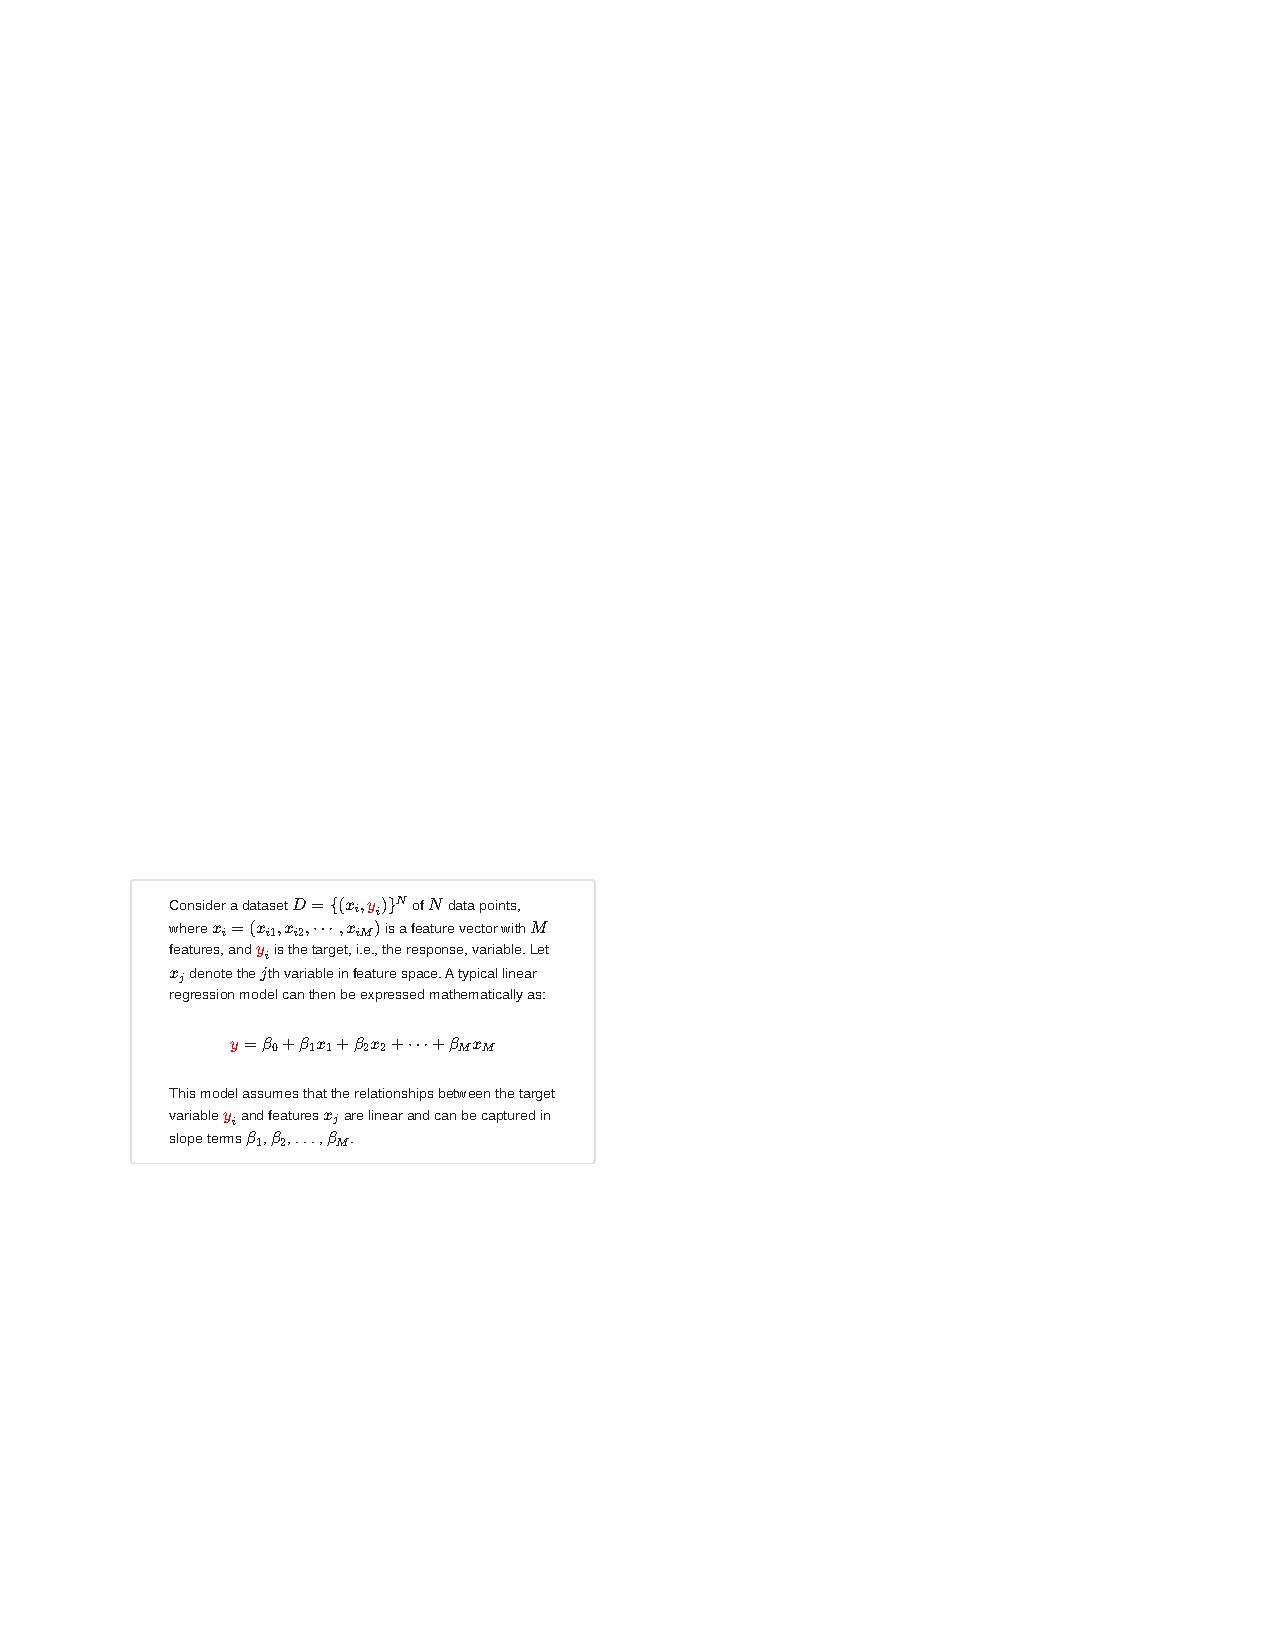
\includegraphics[width=1.02\linewidth]{fig/P4-3.pdf}} }{ \demofig{3}\Description{The excerpt of the math text, augmented to color the variable “y” red wherever it appears in the block formula, inline formulas, and text.} } 

The next step is to use color to help readers find the description of $y$ in the text.
\zed{As Auggie is writing in a web-based environment, they can mix in some CSS to format the text. The CSS can be written alongside the FFL.}
\zed{To style the text,} Auggie surrounds the definition phrase with a \texttt{span} tag and gives it the class ``\texttt{target}.'' Then they give the definition the same color by adding \zed{a selector for the span}, ``\texttt{*.target}'', next to the FFL selector. \\[1ex]
\aptLtoX[graphic=no,type=html]{ \centerline{
\includegraphics[width=1.02\linewidth]{fig/P4-4.pdf}} }{ \demofig{4}\Description{An updated FFL augmentation specification. The selector “star-dot-target” has been added to the list of selectors that will be formatted with the same red color as above.}\\[-1ex] } 
\aptLtoX[graphic=no,type=html]{ \centerline{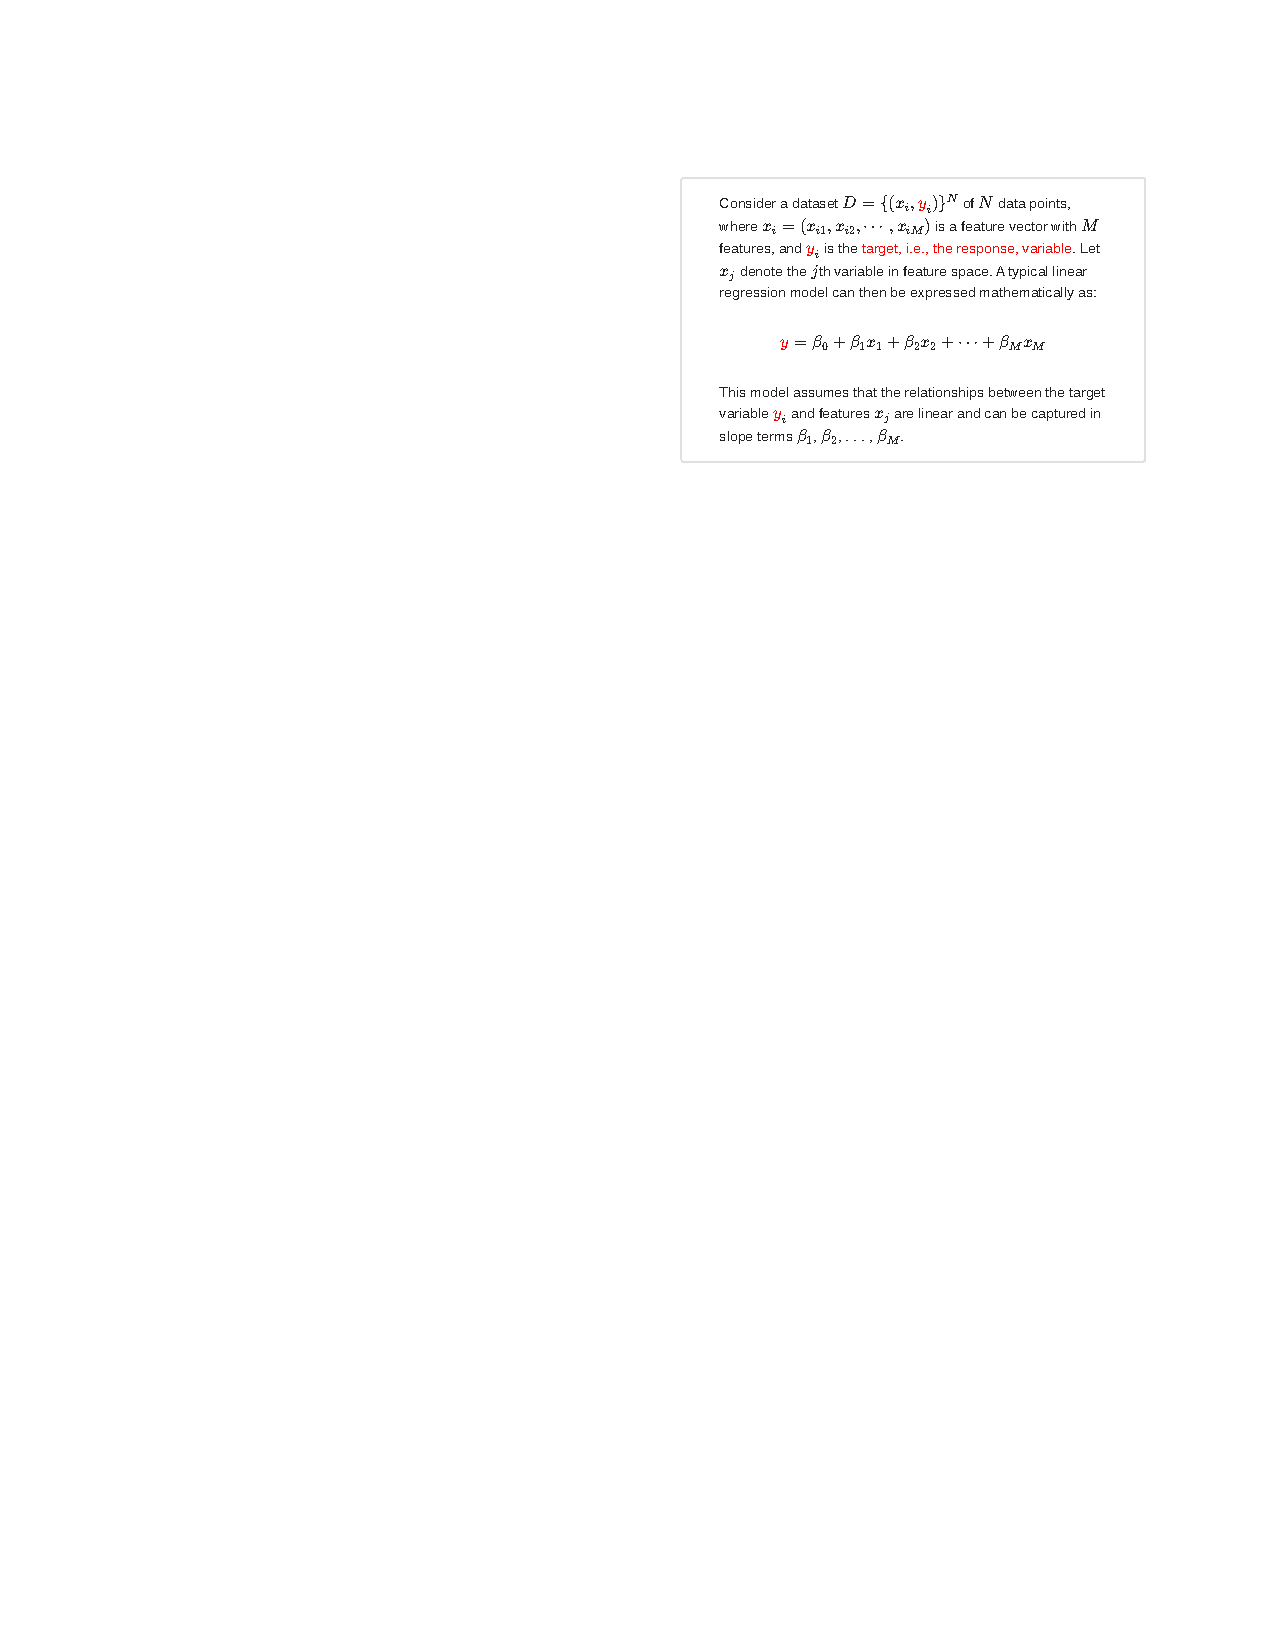
\includegraphics[width=1.02\linewidth]{fig/P4-5.pdf}} }{ \demofig{5}\Description{The excerpt of the math text, with the span of text with the “target” class colored red. This newly-highlighted text reads “target, i.e., the response, variable.”} } 


Auggie is not content with the augmentation, wishing to try out other, less harsh colors. As they experiment with other colors from \texttt{DarkRed} to \texttt{Crimson}, they see the visual effect live, 
receiving the rapid feedback common to online Markdown editors, but less common to LaTeX document editors that require recompilation. \\[1ex]
\aptLtoX[graphic=no,type=html]{ \centerline{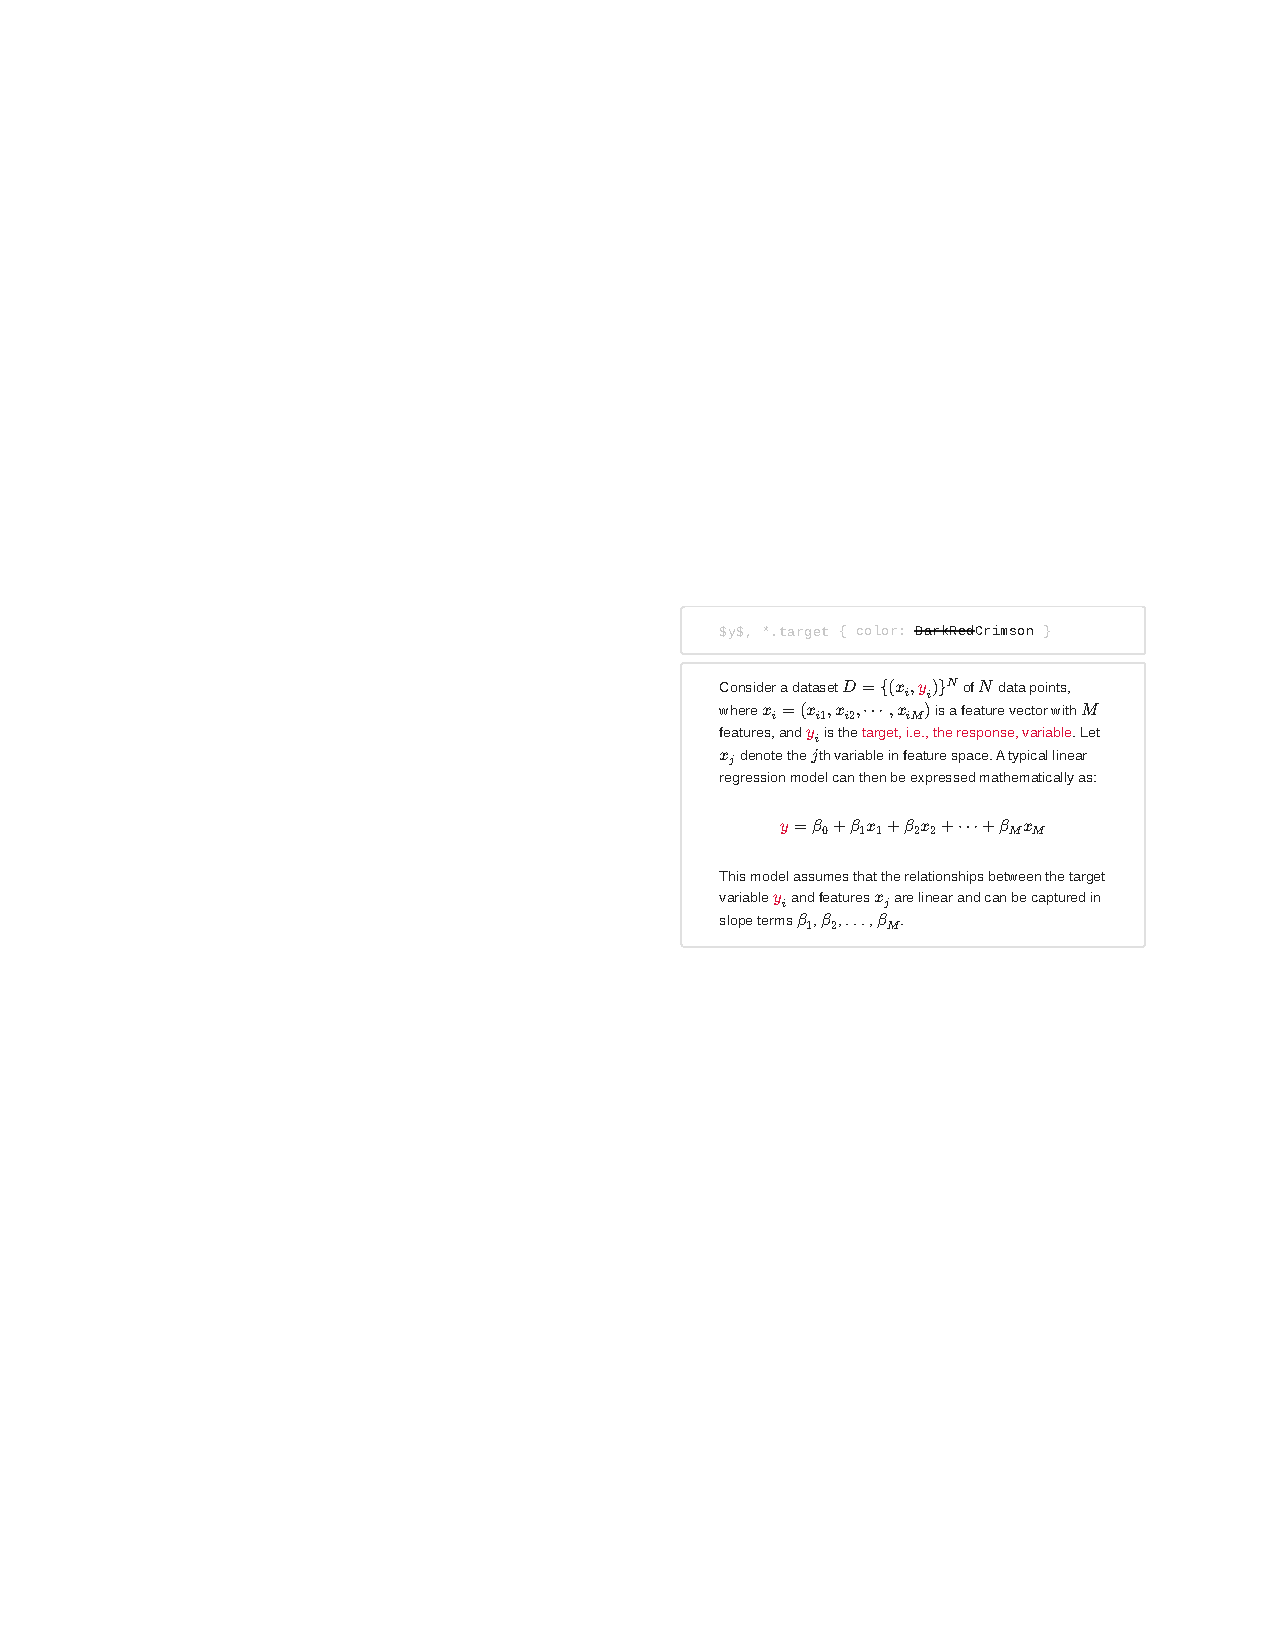
\includegraphics[width=1.02\linewidth]{fig/P4-6.pdf}}}{ \demofig{6}\Description{An updated FFL augmentation specification. The color property has been changed first to DarkRed, and then to Crimson.}\\
\demofig{7}\Description{The excerpt of the math text, where the text that was colored red before is now colored crimson.} } 


Now that Auggie is content with the colors they chose, they notice that they wish for the subscripts of $y$ expressions to be colored as well. To augment all $y$ expressions with subscripts, Auggie only needs to make a small edit.
They add ``\texttt{\$y\_*\$}'' to the list of selectors, and see the crimson color applied to the intended expressions. \\[1ex]
\aptLtoX[graphic=no,type=html]{ \centerline{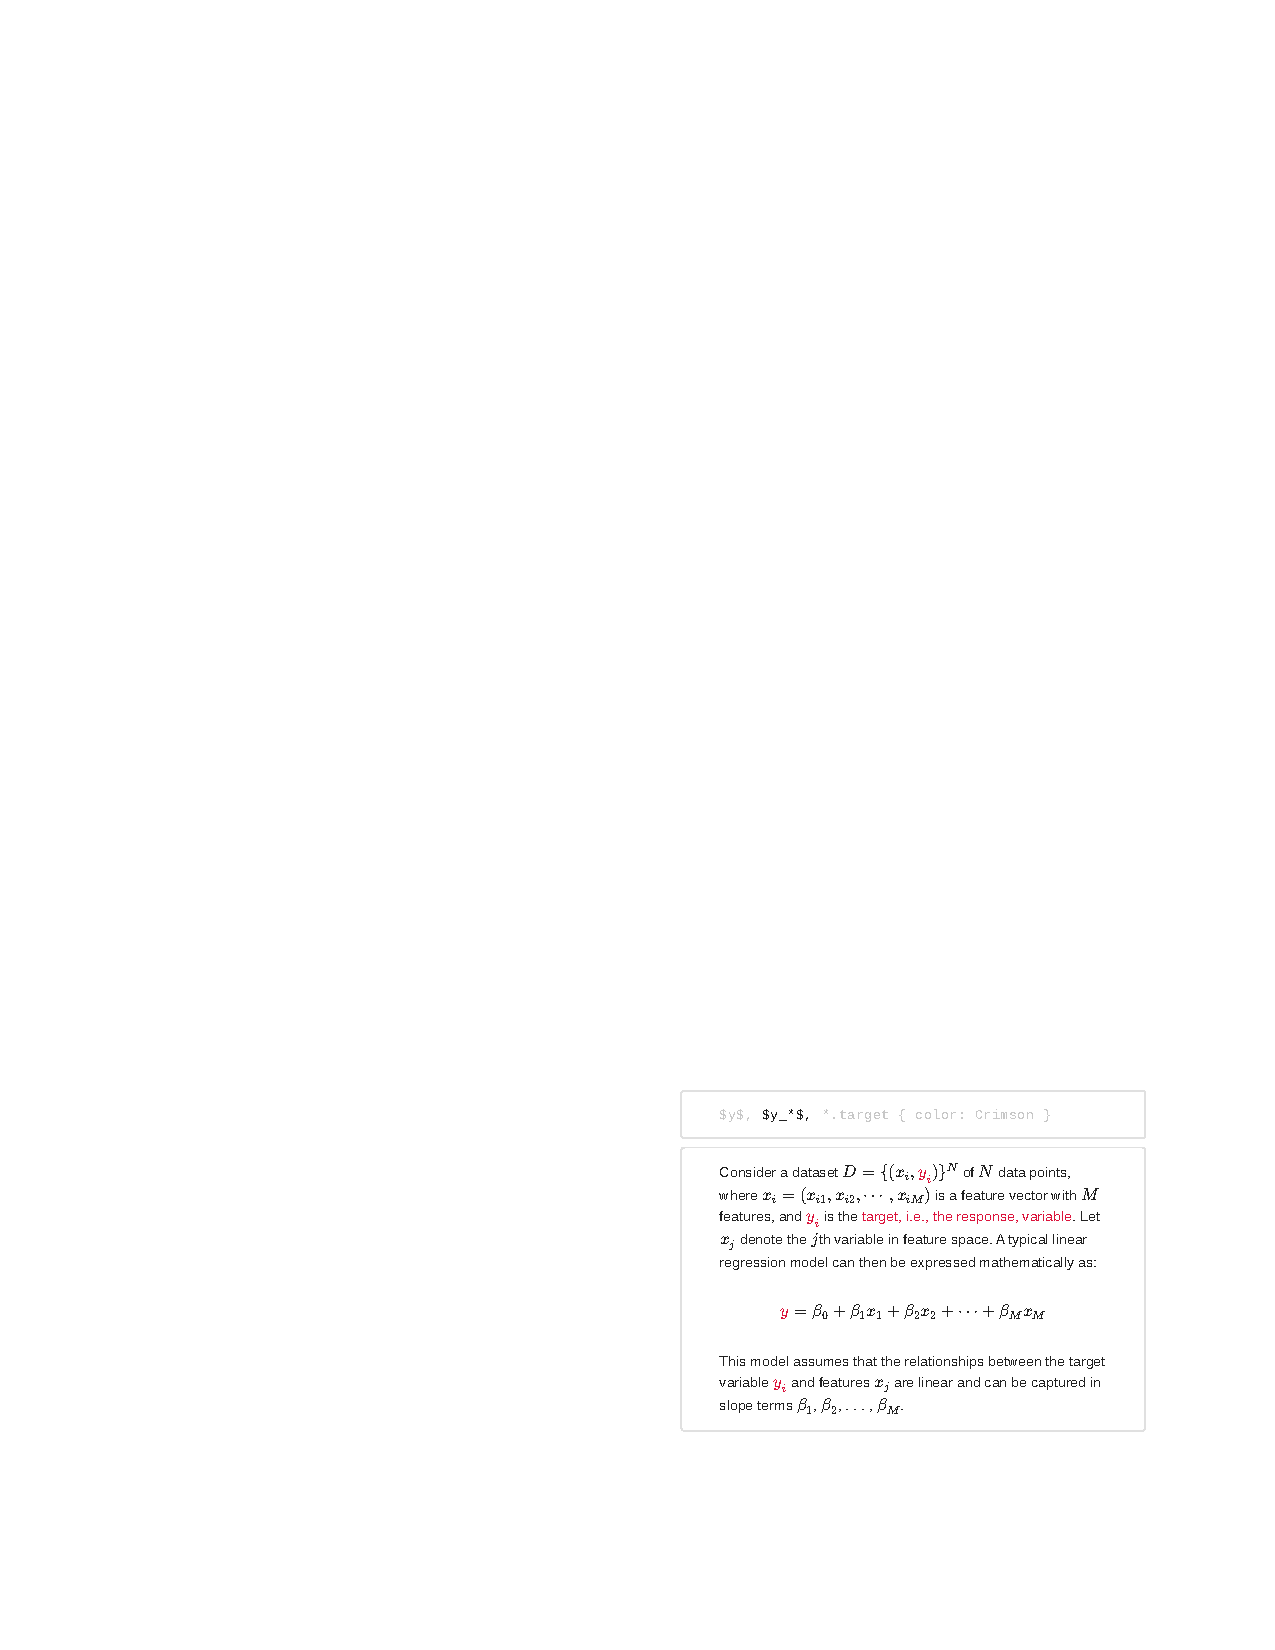
\includegraphics[width=1.02\linewidth]{fig/P4-7.pdf}} }{ \demofig{8}\Description{An updated FFL augmentation specification. The selector “dollar-sign-y-underscore-start-dollar-sign” has been added to the list of selectors that will be formatted with crimson color.}\\
\demofig{9}\Description{The excerpt of the math text, with all symbols consisting of “y” and a subscript are now colored crimson as well.} } 


The next step is to help readers understand the other major expressions in the formula, namely the $x$'s (\textcolor[HTML]{005A9C}{{blue}}) and $\beta$'s (\textcolor[HTML]{9370DB}{{purple}}). Auggie decides to assign each a distinct color that will help a reader look up the respective definitions in the text. To do so, they create a similar style block for each group of variables they wish to augment:\\[1ex]
\aptLtoX[graphic=no,type=html]{ \centerline{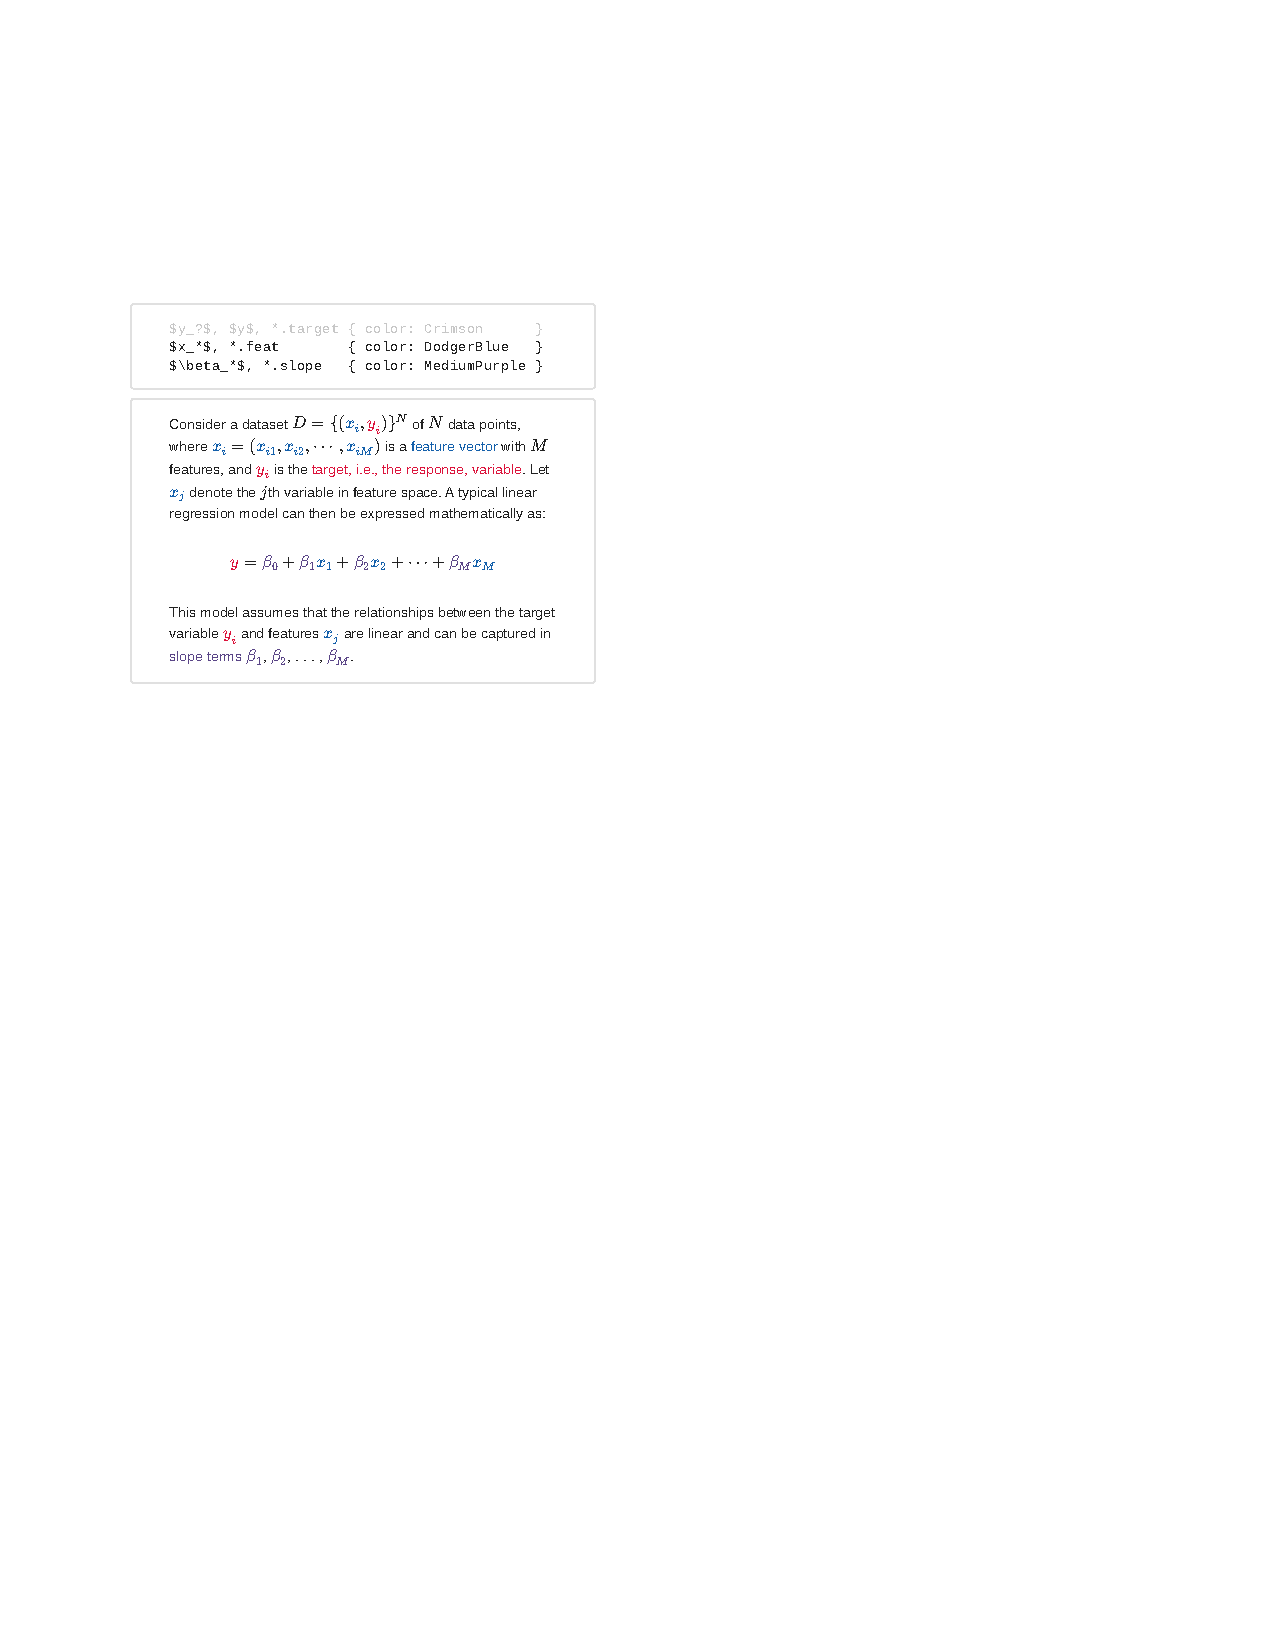
\includegraphics[width=1.02\linewidth]{fig/P5-1.pdf}} }{ \demofig{10}\Description{An updated FFL augmentation specification. Two new augmentation rules have been added. The first rule consists of a selector for “dollar-sign-s-underscore-star-dollar-sign” and “star-dot-feat”, and a property to color matching expressions “DodgerBlue”; and a selector for “dollar-sign-beta-underscore-star-dollar-sign” and “star-dot-slope,” and a property to matching expressions MediumPurple.}\\[-1ex]
\demofig{11}\Description{The excerpt of the math text, with a few changes. All symbols related to “x,” and the phrase “feature vector” are colored with the color “DodgerBlue.” All symbols related to “beta” and the phrase “slope terms” are colored with the color “MediumPurple.”} } 


After inspecting the augmented passage, Auggie wishes that $\beta_0$ was not given the same color as the other $\beta$ terms, because it is better described as an intercept rather than a slope term. They revert the style for just $\beta_0$ by adding an additional one-line rule, setting the color of $\beta_0$ to \texttt{inherit}, as one might do in CSS, rather than accept the color of the other $\beta$ terms.\\[1ex]
\aptLtoX[graphic=no,type=html]{ \centerline{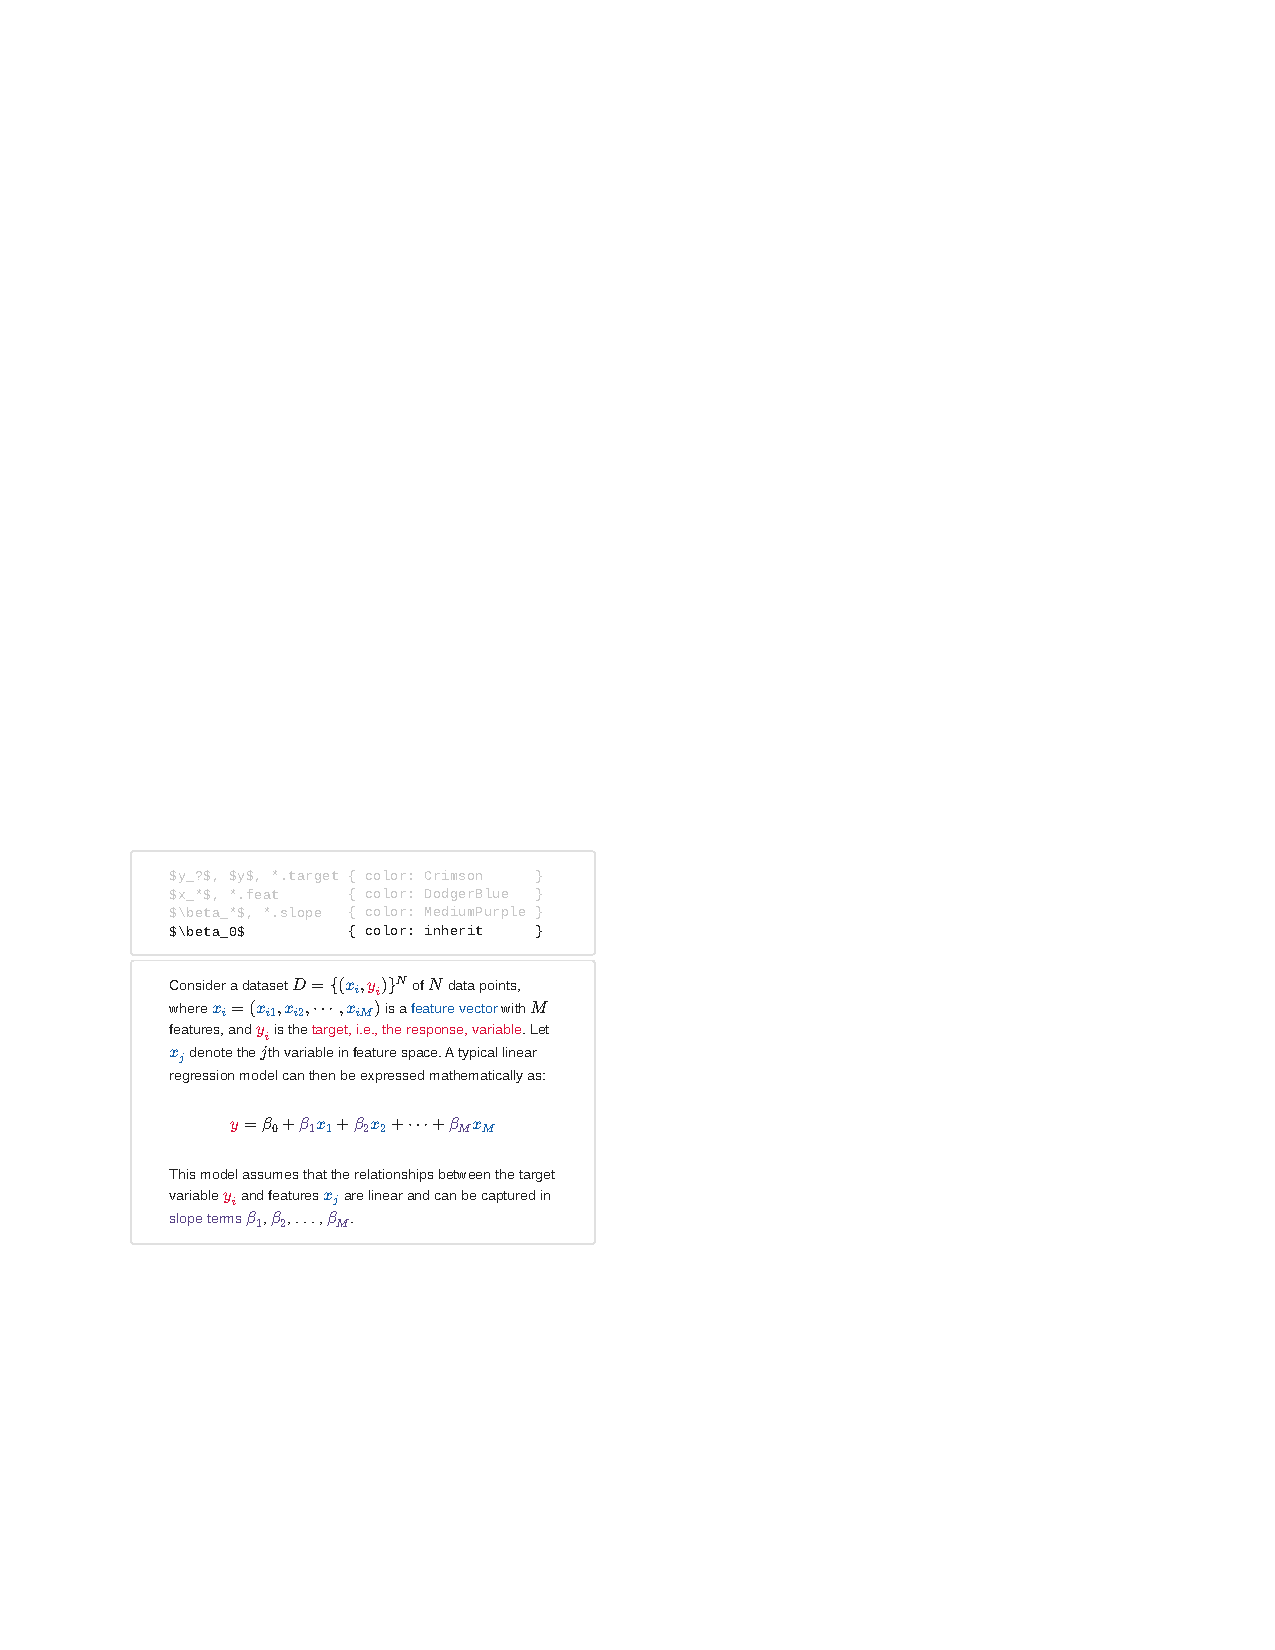
\includegraphics[width=1.02\linewidth]{fig/P5-2.pdf}} }{ \demofig{12}\Description{An updated FFL augmentation specification. One new augmentation rule has been added. The selector is “dollar-sign-beta-subscript-zero-dollar-sign,” and the accompanying style property is “color” with the value “inherit.”}\\\demofig{13}\Description{The excerpt of the math text, this time with “beta-sub-0” colored black instead of purple.} } 

Auggie is satisfied with this result. Throughout their exploration, FFL provided a lightweight syntax for making cross-cutting notation augmentations with live feedback.
% And after only a few simple steps like these, now readers can navigate back to relevant elements in the text just with the colors.

\subsubsection*{Further design space exploration} There is more than one way to augment a formula to expose its meaning. Auggie considers another strategy that they think will make their article more skimmable which relies less on the textual description (omitted below) and instead exposes descriptions of expressions in labels. FFL helps them experiment with this style of augmentation as well.

Auggie starts from a fresh FFL style sheet, this time adding augmentations in the form of labels. They first add a label for $y$, describing it as the ``target'' of prediction.\\[1ex]
\aptLtoX[graphic=no,type=html]{ \centerline{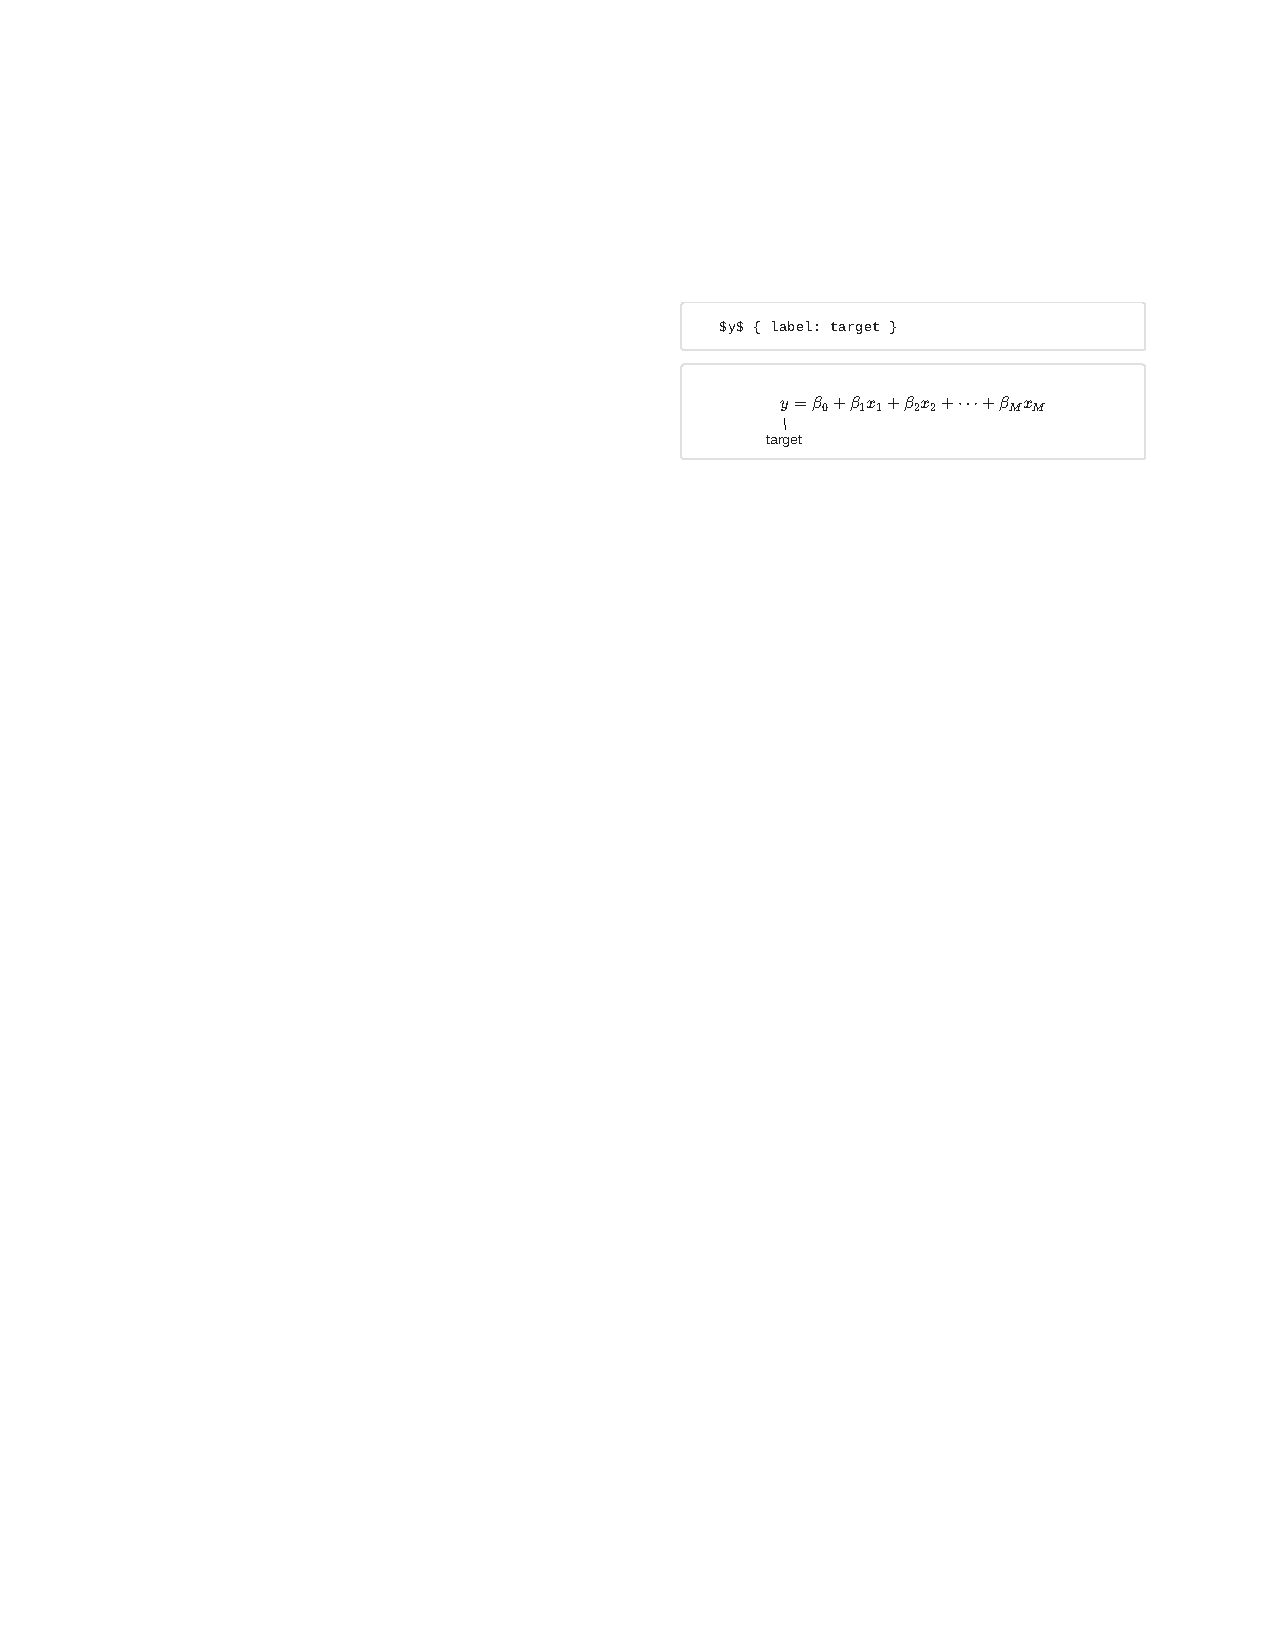
\includegraphics[width=1.02\linewidth]{fig/P5-3.pdf}} }{ \demofig{14}\Description{A new FFL augmentation specification, with the selector “dollar-sign-y-dollar-sign,” and the property “label” with the value “target.”}\\[0ex]
\demofig{15}\Description{The linear regression formula with “y” labeled with the word “target.”} } 

They then add labels for the remaining expressions. This is a matter of adding one style block per annotated expression. \\[1ex]
\aptLtoX[graphic=no,type=html]{ \centerline{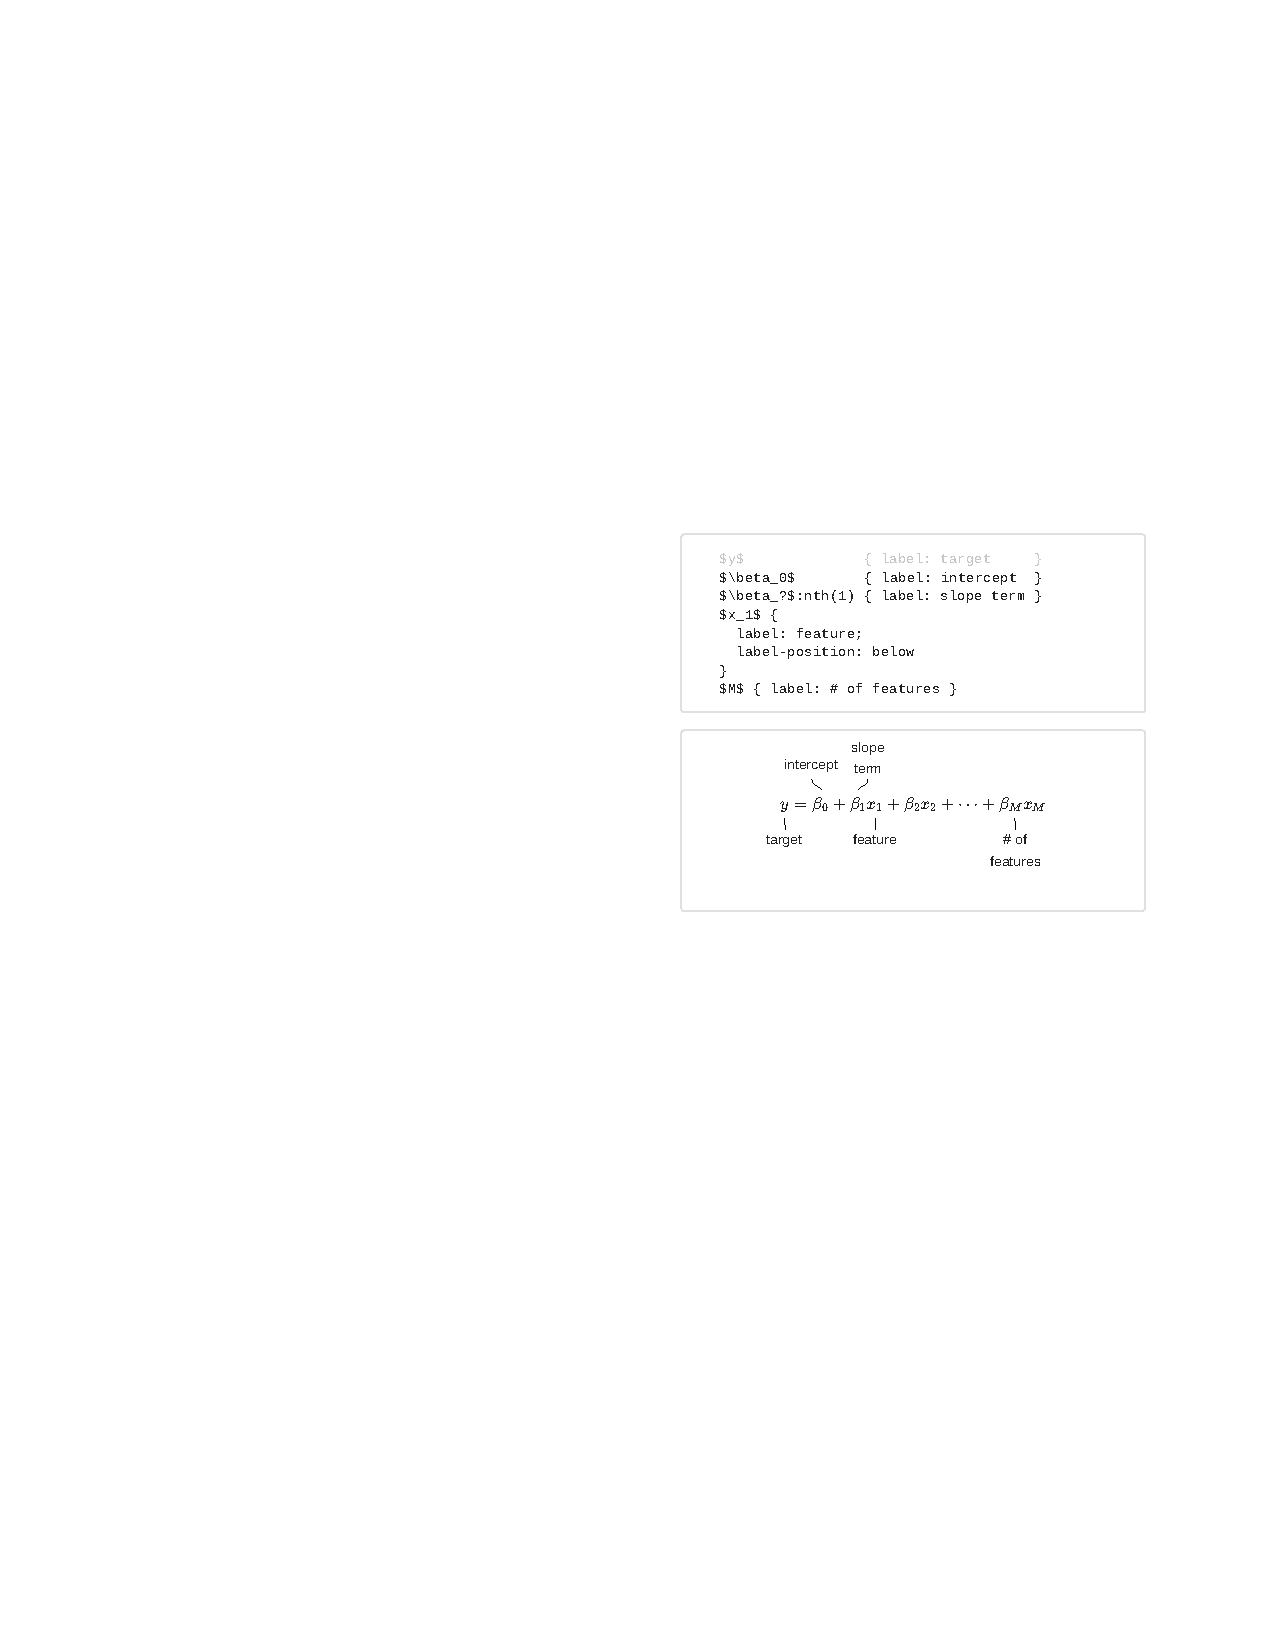
\includegraphics[width=1.02\linewidth]{fig/P5-4.pdf}} }{ \demofig{16}\Description{An updated FFL augmentation specification, extended with rules for adding labels for 4 additional expressions. Each rule consists of the label property and a value of what the label should read. One of the selectors uses the “label-position” property to specify the label should appear “below” the formula.}\\
\demofig{17}\Description{The linear regression formula with labels as follows: “y” is labeled “target”; “beta-sub-0” is labeled “intercept”; “beta-sub-1” is labeled “slope term”; “x-sub-1” is labeled “feature” and the label appears below the expression; “beta-sub-M” is labeled “number of features.”} } 

The labels render live as Auggie does so. The labels are automatically laid out to reduce overlap and maximize adjacency of labels to expressions. In this way, Auggie can think about augmentations at a high level, avoiding the work of manually arranging labels. Notably, the labels are tolerant to future changes to the formula: should Auggie add additional $\beta$ and $x$ terms to the formula, the labels will move as the formula adjusts its position. 
% And this above is all they need to write. No more low-level ``drawing'' commands because it is just \texttt{label} in FFL; No more meticulously shifting labels around to make space for new ones because FFL spaces them automatically; And again, there is no need to wait for compilation to confirm that their positions are as intended. \\

When they are finished with this document, Auggie could save their style sheet for use in other documents with notation that deserved to be described in similar ways.

\section{System}

In this section, we describe FFL, a language and live runtime for augmenting typeset math formulas in web documents. FFL was designed and developed following an iterative approach. Fine-grained decisions about syntax design were informed by pilot usability studies with early versions of the tool.

Acknowledging the challenges of writing augmentation markup revealed in prior work~\cite{ref:head2022math}, the goals of FFL were as follows:

\begin{itemize}
\item Basic augmentations should be easy to read and write;
\item Authors should receive rapid feedback on their designs;
\item Augmentations should be aesthetically pleasing;
\item Authors should be supported to experiment with cross-cutting augmentation choices.
% \item \textit{Interactivity}: Our tool should allow dynamic representation of formula;
% \item \textit{Ease of Use}: Basic styling should be easy to both implement and understand;
% \item \textit{Pretty Defaults}: It should not require a massive amount of tweaking to achieve usable results; and
% \item \textit{Reusability}: Configurations should be able to be reused to make cross-cutting or repeated styling elements.
\end{itemize}

Below, we describe the two main components of the FFL toolkit: the language, and the supporting live runtime.

% FFL comprises the following main components:
% \begin{enumerate}
%     \item A language similar to CSS for selecting and augmenting math expressions;
%     \item A runtime that supports the live application of styles to formulas that are typeset using the popular KaTeX web formula renderer.
% \end{enumerate}

\subsection{Language design}

% \andrew{It feels important for us to note in the text that we don't think that the current specification of FFL is complete, but rather a starting point for a more comprehensive set of augmentations. The main parts of the language---of selectors, styles, and annotations---is our major contribution, as well as the development of what we think are going to be the most powerful, general-purpose features.}

\begin{figure*}
    \centering
    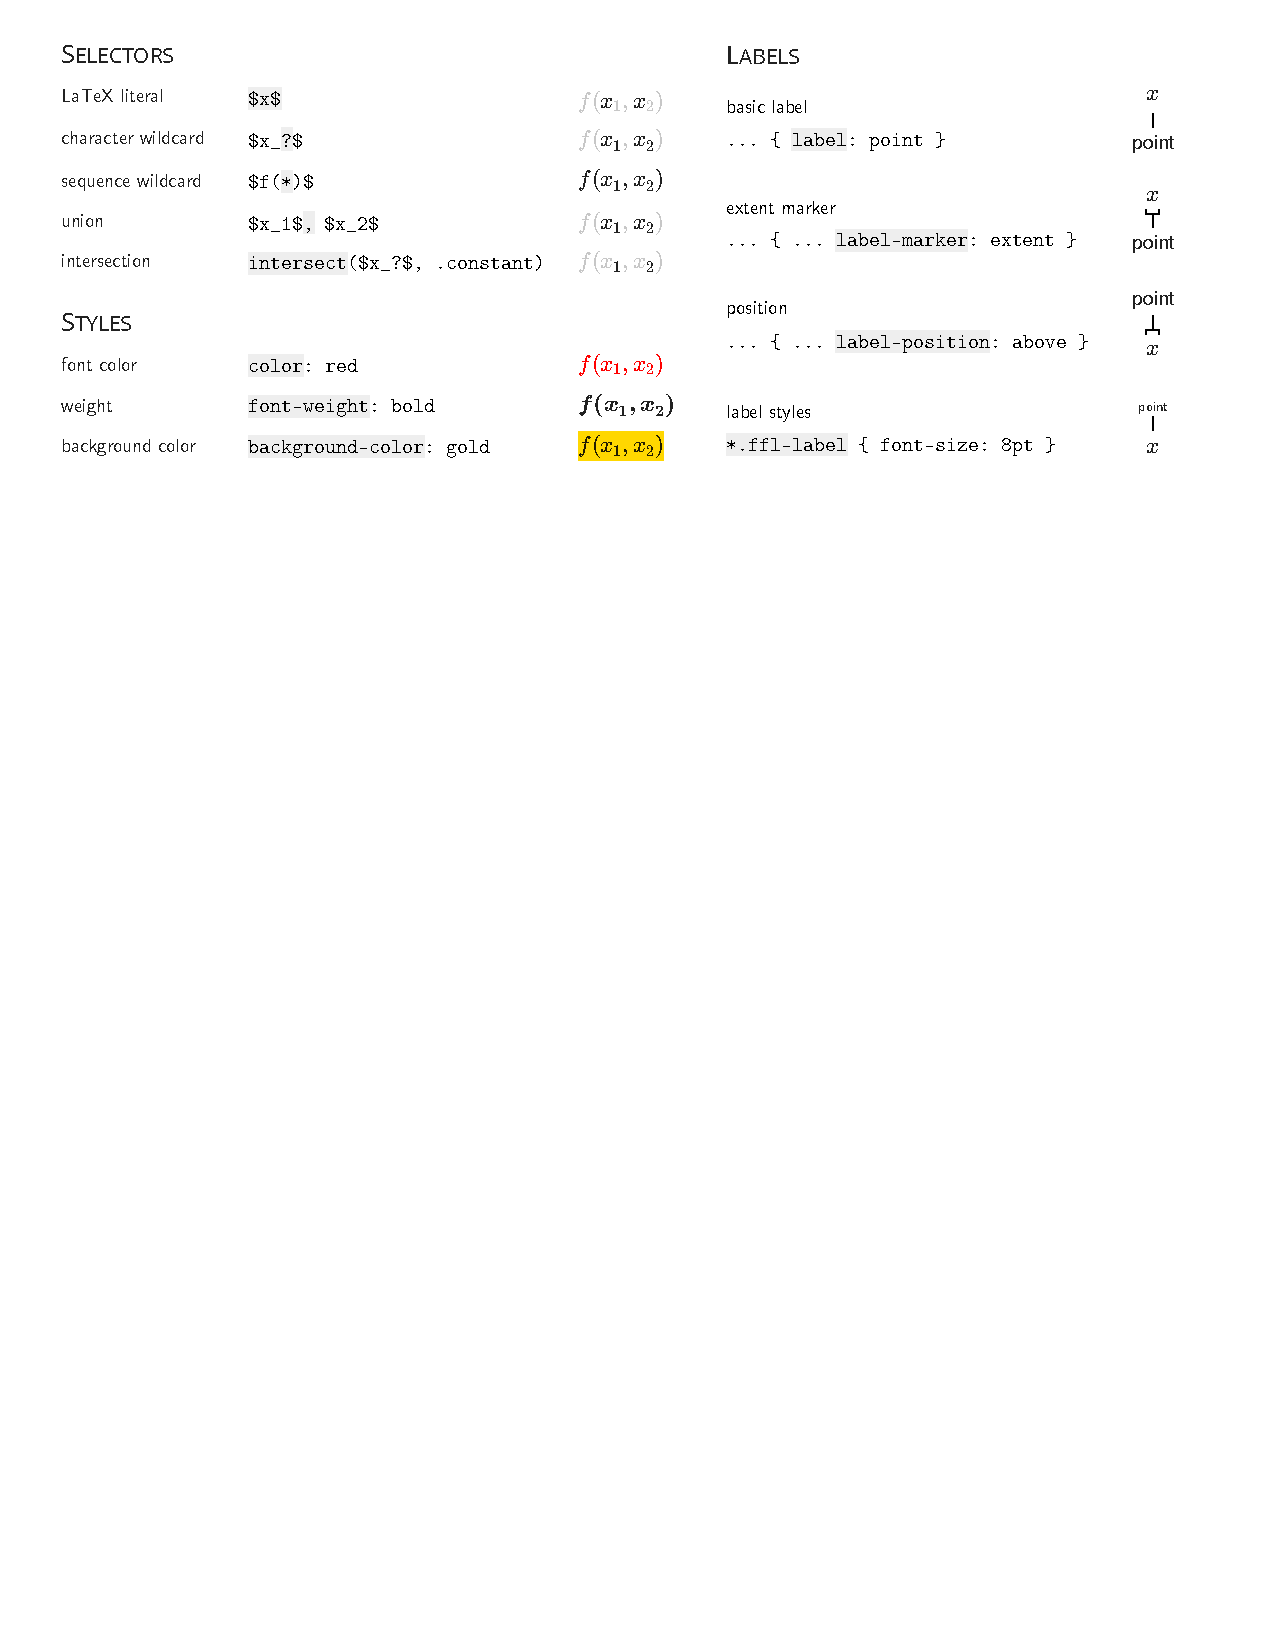
\includegraphics[width=.95\linewidth]{fig/Language}
    \caption{A visual specification of the FFL language, including its constructs for selecting expressions, styling, and labeling formulas. \normalfont Each row names a language feature, provides an example snippet of FFL, and shows the result of its application to one of the example formulas $f(x_1, x_2)$ or $x$.}
    \Description{A table showing features of the FFL language. In each row is the name of the feature, an example of an FFL spec using that language features, and a render of a formula that has been augmented with that spec. Features include: for selectors: literal selectors, character and sequence wildcards, union, and intersections. For styles: font color, weight, and background color. For labels: simple labels, extent markers, label positions, and additional styles.}
    \label{fig:language_examples}
\end{figure*}

% \andrew{Figures: @Zed, what is your current thinking around having a BNF declaration of the language?} probably more formal than we need to be since we already have the feature figure

The FFL language is a CSS-like language for specifying augmentations for formulas. FFL was designed to resemble CSS due to the latter's use as a separable styling language in web authoring environments. We envisioned authoring environments where eventually authors write FFL and CSS side-by-side.

\begin{wrapfigure}[5]{l}{0.25\columnwidth}
\vspace{-2ex} % TODO: fix to fit any new position
\begin{Verbatim}[commandchars=\\\{\}]
 \textcolor{darkblue}{$x_i$}, \ldots \{
   \textcolor{magenta}{ color: red; }
   \textcolor{magenta}\ldots
 \}
\end{Verbatim}
\end{wrapfigure}
Like CSS, FFL in essence consists of declarations of style rules. Each style rule block consists of a \textcolor{darkblue}{selector} indicating what expressions the augmentation applies to, and a set of \textcolor{magenta}{property declarations} describing augmentations to apply, resembling the inset figure.

One advantage of this format is that FFL can be easily transpiled to CSS for a myriad of simple styles (e.g., color, font weight). Below demonstrates the current expressive potential of FFL's syntax. A visual summary of language constructs appears in Figure~\ref{fig:language_examples}. Our focus is to describe the language primitives, and the augmentations we have built into the language to date. We intend the language to be further extended to support additional augmentations.

\subsubsection{Selections}
An author conveys which math expressions to augment by writing \emph{selectors}. FFL provides a flexible selector syntax, allowing for literal matches to LaTeX substrings, wildcards, predefined classes, and combinators.

\paragraph{Literal Selectors} The simplest way to select an expression is to write the LaTeX for the expression one wishes to augment. Writing a literal selector entails writing a LaTeX string, with its typical (\texttt\$) delimiters on either side. Literal selectors are resilient to some simple variations in how an expression might be written in LaTeX: for instance, the selector ``\texttt{\$x\_i\$}'' matches the expression $x_i$ regardless of whether it is written ``\texttt{\$x\_i\$}'' and ``\texttt{\$x\_\{i\}\$}''.

\paragraph{Wildcards} Authors can select syntactically related expressions using wildcards. Two kinds of wildcards are provided, inspired by the \texttt{glob}~\cite{UnixMan} wildcard syntax used in Unix command lines. \emph{Character wildcards} match single characters, and are written ``\texttt{?}''. For instance, ``\texttt{\$x\_?\$}'' selects all symbols that have $x$ as a base and a single character as subscripts. \emph{Sequence wildcards} match strings of unbounded length, and are written ``\texttt{*}''. For instance, ``\texttt{\$f(*)\$}'' selects $f()$, $f(0)$, $f(x)$, and $f(x + 1)$, among other expressions. \zed{Authors can match the literal characters ``\texttt{?}'' and ``\texttt{*}'' by escaping them with a backslash (i.e., as ``\texttt{\textbackslash?}'' and ``\texttt{\textbackslash*}'').}


\aptLtoX[graphic=no,type=html]{ \centerline{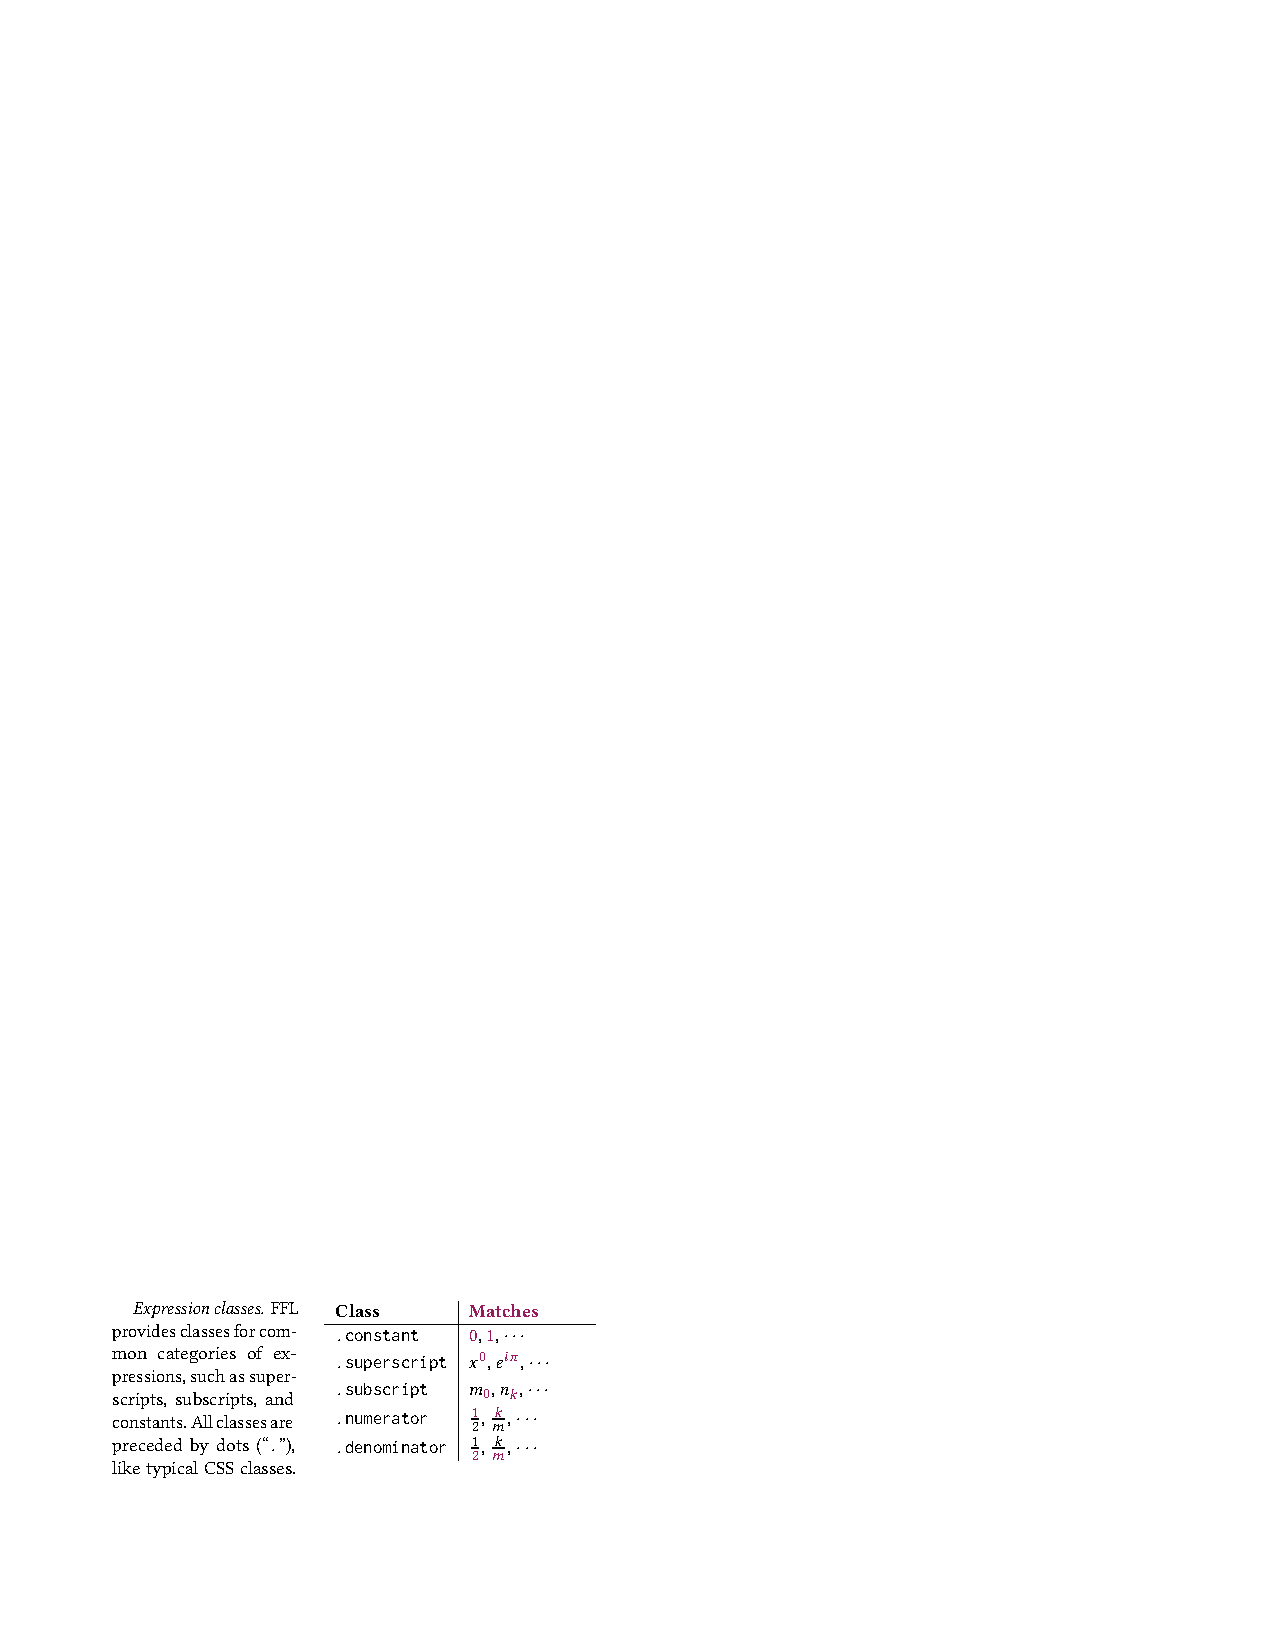
\includegraphics[width=1.02\linewidth]{fig/P6-1.pdf}} }{ \setlength{\columnsep}{1em}%
\begin{wrapfigure}[8]{r}{0.6\columnwidth}
% \begin{center}
    \vspace{-1.4em}
    \hspace{1ex}
    \begin{tabularx}{.54\columnwidth}{l|l}
    \textbf{Class}   & \textcolor{magenta}{\textbf{Matches}}                                 \\\hline
    \texttt{.constant}    & $\textcolor{magenta}{0}$, $\textcolor{magenta}{1}$, $\cdots$                     \\[2pt]
    \texttt{.superscript} & $x^{\textcolor{magenta}{0}}$, $e^{\textcolor{magenta}{i\pi}}$, $\cdots$          \\[2pt]
    \texttt{.subscript}   & $m_{\textcolor{magenta}{0}}$, $n_{\textcolor{magenta}{k}}$, $\cdots$             \\[2pt]
    \texttt{.numerator}   & $\frac{\textcolor{magenta}{1}}{2}$, $\frac{\textcolor{magenta}{k}}{m}$, $\cdots$ \\[2pt]
    \texttt{.denominator} & $\frac{1}{\textcolor{magenta}{2}}$, $\frac{k}{\textcolor{magenta}{m}}$, $\cdots$ \\
    \end{tabularx}
    \Description{A table of predefined classes, where each row shows the name of the class and examples of expressions the class matches. Every class name is preceded by a period. “dot-constant” matches numerical constants like 0 or 1. Superscripts, subscripts, numerators, and denominators match the mathematical structures of the same name.}
% \end{center}
\end{wrapfigure} } 


\paragraph{Expression classes} FFL provides classes for common categories of expressions, such as superscripts, subscripts, and constants. All classes are preceded by dots (``\texttt{.}''), like typical CSS classes. Supported classes are shown in the inset figure. These classes become particularly powerful when used within combinators, permitting an author to select, for instance, squares as the appearance of the literal ``\texttt{$2$}'' within superscripts.

\paragraph{Indexed groups} To disambiguate between selections, we offer another special class named ``\texttt{.group}'', referring to portions of the formula markup surrounded by double braces (e.g. \texttt{\{\{}\dots\texttt{\}\}}). \zed{The modifier ``\texttt{:nth($i$}\texttt{)}'' can be appended to any selector to select the $i$-{th} matching expression. Authors select a specific group by using the modifier in conjunction with the ``\texttt{.group}'' selector. }

\paragraph{Combinators}
Selectors can be composed to make them more general or more precise. Selections can be made more precise with the intersection combinator, ``\texttt{{intersection}(}{\textit{selector1}, \textit{selector2}, \textit{...}}{\texttt{)}},'' which selects expressions matching all selectors provided as arguments. A shorthand for intersection is provided as ``\texttt{\textit{selector1} \textit{selector2} \textit{...}},'' which is reminiscent of CSS's compound selectors; with this shorthand authors can express intersections as if they were selecting \texttt{selector2} from within \texttt{selector1}. The union combinator, as with CSS, uses a comma (``\texttt{,}'') to separate selectors, matching any expression that matches one of the selectors.

\paragraph{CSS Selectors} To select HTML elements from within an FFL style specification, an author can prepend an asterisk (``\texttt{*}'') to the name of a class (e.g., ``\texttt{*.cls0}'').

\subsubsection{Augmentations}

The FFL language supports specification of two kinds of augmentations: styles and labels. Permitted augmentations include color and labels, the two most commonly used kinds of augmentations according to a recent survey~\cite{ref:head2022math}.\footnote{An analysis of the spreadsheet in Head et al.'s~\cite{ref:head2022math} supplemental material shows 69\% of augmented formulas in their sample made use of either font color or labels.}
% Check or extend my work here: https://docs.google.com/spreadsheets/d/1YE7mw6Xrw6ebleQrfe13q2vv_0-J-Y1gPODhrhgwlrA/edit#gid=763614481

\paragraph{Style}
Styles are alterations to the expression elements, like color, font weight, and background. They correspond roughly to CSS properties, and share the same names (e.g., ``\texttt{color},'' ``\texttt{font-weight}''). Because these properties are transpiled into CSS, they accept all of the same property values as CSS (e.g., colors can be specified using HTML color codes, hex codes, ``\texttt{rgba(}\dots\texttt{)}'' values). As described in Section~\ref{sec:overlays}, some styles require additional processing on the backend to provide the expected styling behavior in the unique setting of HTML typeset math formulas.

\paragraph{Labels}
FFL provides language primitives for creating and customizing labels that describe expressions. The ``\texttt{label}'' property allows an author to define and show a label for an expression: upon specifying this property, a label will appear next to the first appearance of that expression in a formula, connected to that expression with a leader line. The ``\texttt{label-marker}'' property allows the author to specify what kind of marker should connect the label to the expression. The marker can be either a \texttt{leader} line or an \texttt{extent} marker, i.e., a bracket shown in the margin; extent markers are particularly useful for labeling long expressions.

Label placement is automatic, and is designed to avoid overlapping labels and to place labels as close to their corresponding expressions as possible. \zed{A label is applied only once to any given formula; it is anchored to the first appearance of the labeled expression.} Should an author wish to customize the placement of labels, they may do so by defining the ``\texttt{label-position}'' property to place the label either ``\texttt{above}'' or ``\texttt{below}'' the formula.  To support further label customization, all labels allow values of ``\texttt{html(}\dots\texttt{)}'' (sanitized for security by default), or are generated as HTML text \texttt{span}s with the class ``\texttt{ffl-label}'' class. In this way, their appearance (e.g., font size, font family, color) can be configured with normal CSS properties by using the CSS selector ``\texttt{*.ffl-label}.''

\subsection{Live runtime}

FFL was designed to be incorporated into arbitrary web-based text editing tools as a live styling utility, and for integration into articles generated from these editors. In this section, we describe how the runtime supports integration as a live styling tool.

\subsubsection{FFL library}

To ease the work involved in integration, FFL is implemented as a light wrapper around widely-used \textit{KaTeX}~\cite{tool:katex} tool. KaTeX is a tool that typesets LaTeX formulas on web pages. It is used in a variety of web-based authoring tools, including Dropbox Paper, Observable, Gatsby, Messenger, and Quill. \zed{It is also one of the supported formula rendering engines in Jupyter Lab~\cite{jupyterlab-katex}}.

To integrate FFL into a web authoring environment, a developer would do the following. First, they would create editor widgets (like text areas) for authors to write FFL in. Second, they would replace calls to KaTeX's formula typesetter with a call to a nearly equivalent API on FFL. That method has the signature:

% \vspace{-.5ex}
\begin{Verbatim}
ffl.render(latex: string, ffl: string,
  renderTo: HTMLElement, options?: KatexOptions): void
\end{Verbatim}
% \vspace{-.5ex}
where ``\texttt{latex}'' is the LaTeX markup for the formula, the ``\texttt{ffl}'' parameter takes in the FFL style specification, ``\texttt{renderTo}'' is a reference to the HTML element into which to render the augmented formula, and ``\texttt{options}'' is an object of KaTeX options for typesetting the formula. If called without a ``\texttt{renderTo}'' target, the method returns the HTML string for the rendered formula.

\subsubsection{Supporting live evaluation}\label{sec:live_evaluation}
To support live evaluation of an FFL style specification in an editing environment, the one necessity is to trigger a new call to ``\texttt{ffl.render}'' whenever the LaTeX or the FFL specification changes.
To demonstrate the feasibility of such an integration, we implemented a Markdown editing environment with live FFL integrated. To develop this environment, we first created a document editor as a simple text area. When authors write Markdown in the text area, the Markdown is passed to the \textit{markdown-it}~\cite{MarkdownIt} open source Markdown parser and then rendered into a document view next to the Markdown editor.

We created a pluggable \textit{markdown-it} extension to call the FFL API, rather than the KaTeX API, to render math formulas; the FFL API is called with an FFL style specification that authors write in another text box adjacent to the Markdown text box. Live evaluation is supported by triggering a parse of the Markdown when either the Markdown or the FFL specification is edited.  A demo of the authoring environment appears in the accompanying video.

\section{Implementation}\label{sec:impl}

The FFL runtime required an implementation that would translate specifications of augmentations to rendered HTML formulas. Figure~\ref{fig:dataflow} summarizes the translation process and the intermediate representations involved. Here, we briefly describe our implementation of augmentations in the FFL runtime in terms of each time the API is triggered.\footnote{\zed{Our implementation is hosted at \ifreview\textbf{[SEE CAMERA-READY VERSION]}\else\href{https://penn-hci.github.io/ffl}{\texttt{penn-hci.github.io/ffl}}\fi.}}

\begin{figure}
    \centering
    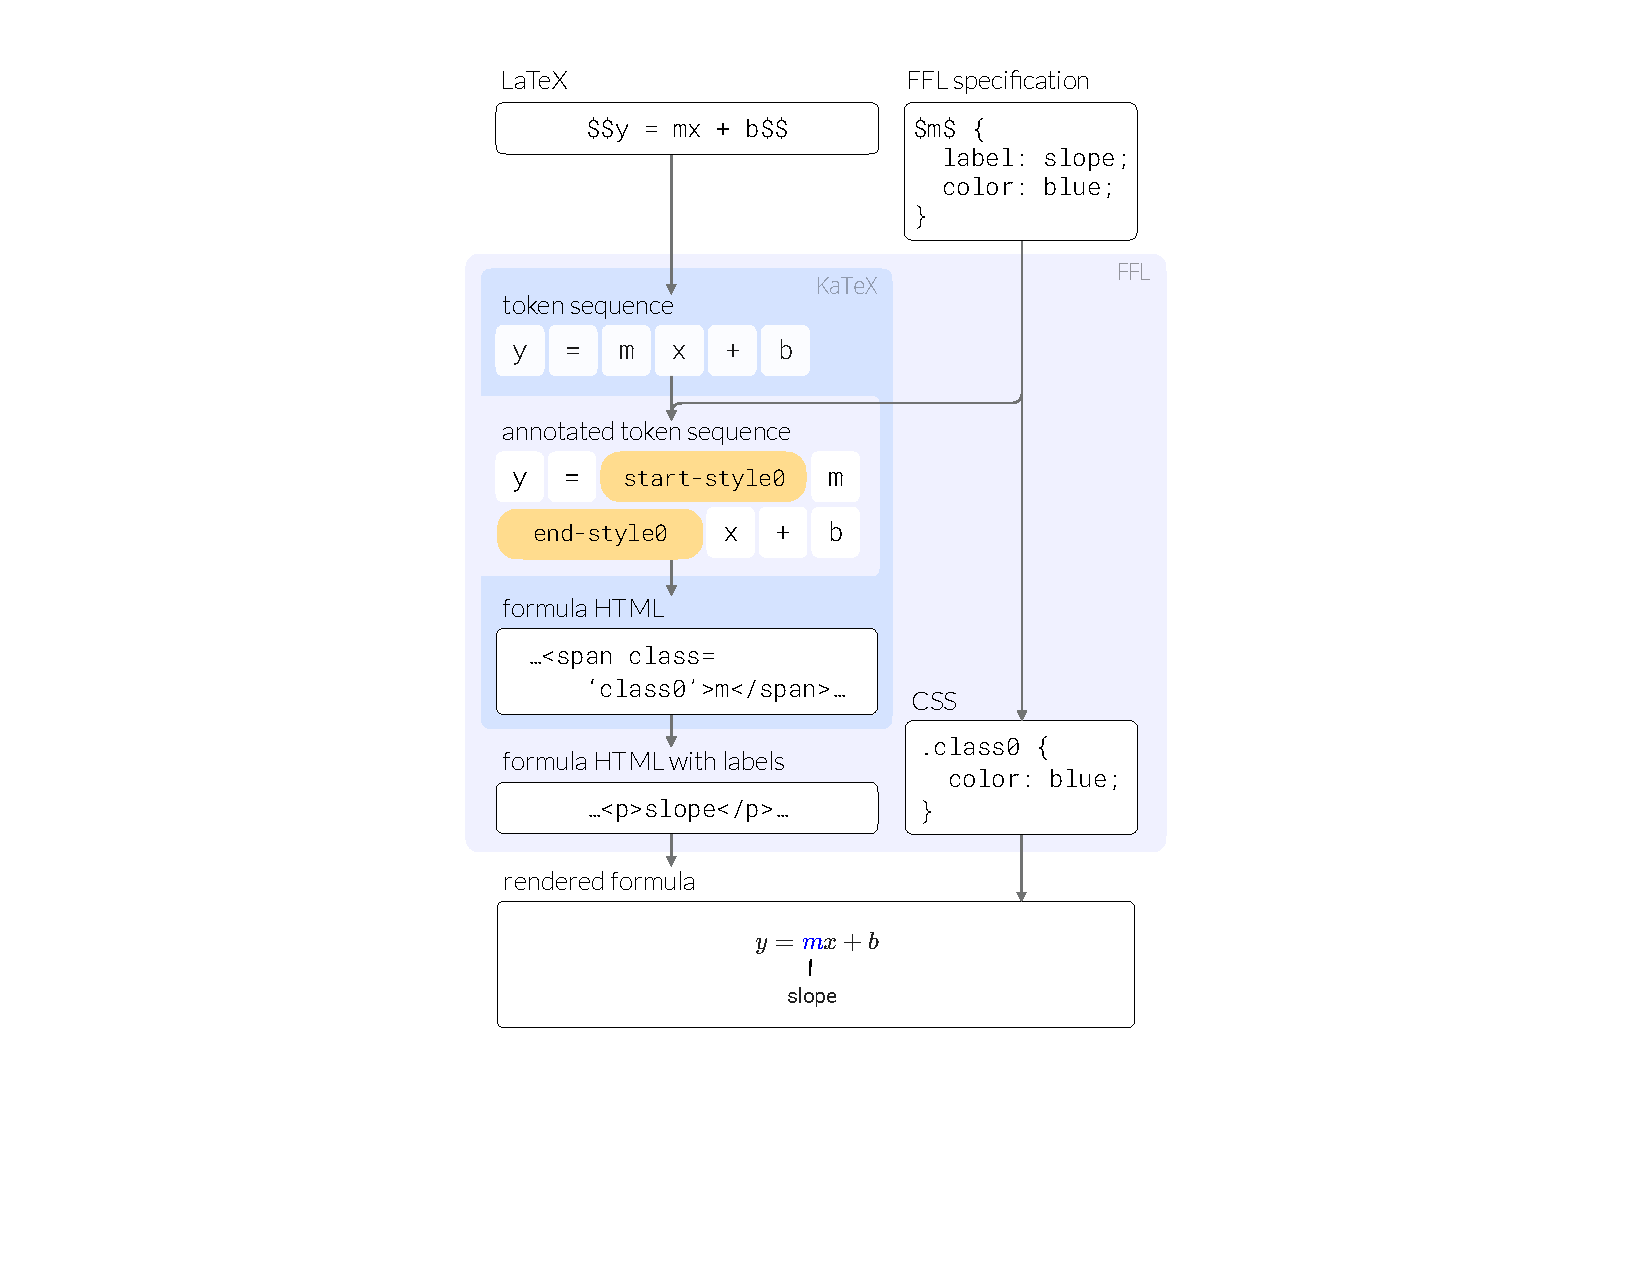
\includegraphics[width=.86\columnwidth]{fig/dataflow} 
    \caption{The generation of an augmented formula from LaTeX and an FFL style specification. \normalfont FFL wraps the  KaTeX library~\cite{tool:katex}, shimming itself into KaTeX's token parsing to detect and annotate expressions of interest. KaTeX generates an annotated HTML formula, which can be styled with CSS that FFL generates from its specification. FFL augments the generated HTML with labels by post-processing the generated HTML.}
    \Description{A decorative flowchart demonstrating how augmented formulas are generated from the LaTeX for a formula and an FFL style specification. The LaTeX math code and FFL style specification are passed into FFL, which then generates CSS from the FFL style specification and passes the LaTeX code to KaTeX, which FFL wraps. KaTeX tokenizes the LaTeX code and lets FFL insert marker tokens to indicate ranges where styles apply, linking the markers to generated CSS classes. KaTeX renders the token stream into HTML. FFL processes the HTML to add label elements. The HTML and CSS are rendered together as an augmented formula by the browser.}
    \label{fig:dataflow}
\end{figure}

\subsection{Parsing the FFL specification}
FFL markup is parsed using a custom parser for the FFL grammar. The parser was generated by Peggy~\cite{Peggy}, a PEG parser generator, from an FFL grammar that resembles a subset of CSS grammar.

\subsection{Matching LaTeX token sequences}
Next, the selectors are used to identify ranges of formula LaTeX that need to be augmented. To do this, we use KaTeX to lex both the selectors and the formula LaTeX into token sequences, with a small amount of parsing to normalize implicit groups. Then, we scan the LaTeX formula token stream for sub-sequences matching the selector, similarly tokenized by KaTeX. \zed{A segment and selector are considered matching if they contain a sequence of matching tokens. Literal tokens are considered matching if they are the same. The wildcards ``\texttt{?}'' and ``\texttt{*}'' match either a single or a sequence of tokens respectively. 
} The current implementation of sub-sequence search permits matching overlapping sub-sequences, and wildcard matches for the character and sequence wildcards.

Once a matching sub-sequence is found, KaTeX must be told to augment the characters in that sub-sequence. To do this, we insert special tokens before and after the sub-sequence. These special tokens instruct KaTeX to insert temporary \texttt{span} tags with a generated class name around the expression in the rendered formula HTML. While it inserts these special tokens, FFL creates a map from FFL selectors to the selector-specific class names, from which it builds a CSS style sheet that applies FFL styles (e.g., color, font weight) to the expression in the rendered HTML formula.

\zed{We implement the search for matching sub-sequences of tokens in a way that does not require changing KaTeX's implementation. Our approach is to handle matching in a custom KaTeX macro that we wrap around each formula. With KaTeX, macros are defined as JavaScript functions. When KaTeX expands a macro, it does so by calling the corresponding JavaScript function, passing the function the sequence of tokens found in the macro's arguments. We wrote a custom macro that, when expanded by KaTeX, takes the tokens of the formula, searches for matching sub-sequences, modifies those sub-sequences as described in the paragraphs above, and returns the modified tokens to KaTeX for further processing.}

\subsection{Applying styles}
Once KaTeX produces the HTML for a rendered formula, FFL traverses the HTML to associate styles with matched expressions. FFL searches for the previously inserted \texttt{span}s, removing them and applying generated CSS class names to the HTML elements between them. Then, it appends the generated CSS (including color and font weight) to a ``\texttt{style}'' element in the DOM, which has the effect of styling the matched elements in the expression.

\subsection{Drawing overlays and underlays}\label{sec:overlays}
Finally, all remaining kinds of augmentations collected during the HTML tree traversal are applied, including labels and background colors. Labels are drawn as relatively positioned HTML elements on the margins of the formula inside an SVG~\cite{tool:svg} element. Label positions are determined by locating the position and outer bounding box of all tokens in its corresponding expression. Label positions are adjusted to reduce overlap by Labella~\cite{tool:labella}. The formula is padded with additional space so that labels do not occlude the surrounding text. Background colors are implemented as relatively positioned boxes placed behind the corresponding expression; this implementation is necessary to support background colors for selections whose constituent elements have a joined area that differs from the rectangular bounding box of the whole expression to ensure that there is only one background box, rather than multiple overlapping boxes for each character element in the expression.

\subsection{Technical limitations}\label{tech-limitations}

Our current technical approach suffices for reifying the ideas behind FFL in a working tool. Here, we describe technical limitations that should be addressed to increase FFL's flexibility and robustness.

\paragraph{Behavior of sequence wildcard} One revelation from our development was that the \texttt{glob}-style ``\texttt{*}'' wildcard is not well-defined for strings with the inherent hierarchy of LaTeX formulas. The current behavior of ``\texttt{*}'' is to match any terminal token or group at the same group level as the ``\texttt{*}'' in the selector. This decision remains to be more closely examined.

\paragraph{Block styles}
For some styles, FFL transpiles directly to CSS. For others like background color, border, and padding, FFL requires custom solutions. The default approach of FFL is to apply a style to all tokens separately in an expression. Rather, block styling augmentations---like padding---should apply to an expression in whole. To overcome this brittleness for block styling, we believe future versions of FFL should use KaTeX's render to MathML~\cite{tool:mathml} instead of HTML; MathML contains structures that can be more easily detected and augmented for these styles, and has become mainstream into most major browsers earlier this year.

\paragraph{Performance}
\zed{Preliminary tests on a commodity laptop show that rendering a formula with FFL takes tens of milliseconds (i.e., 35ms to augment ``$x$'' in the linear regression formula from Section~\ref{Demo}). This runtime is imperceptible for single augmentations applied to single formulas. Our tests lead us to attribute latency to the time it takes FFL to insert augmentation markers into KaTeX's token stream: latency increases as more matches are found in the formula (e.g., it takes 50ms to augment expressions matching ``\texttt{\$*\$}'' in the same demo formula). As the number of augmentations and formulas grows, adjustments will be required (e.g., optimizations, parallelization) for FFL to continue to deliver instant feedback.}

\section{Evaluation}

To evaluate FFL's impact on the experience of authoring augmentations, we conducted an in-lab usability study. The study was designed to answer the following questions:

\begin{enumerate}
\item How does FFL influence authors' ability to create and edit augmentations?
\item How could tools like FFL be improved to better support formula augmentation?
\end{enumerate}

The study consisted of a controlled comparison between FFL and a LaTeX baseline for augmentation creation and editing tasks, followed by an exploratory authoring task with FFL.

\subsection{Participants}\label{study-participants}

We sought participants with experience authoring math documents with LaTeX. Participants were recruited from graduate student mailing lists at a computer science program at a private university, with the sole prerequisite of prior experience writing LaTeX formulas.

33 participants were recruited in total. The vast majority were master's students; 7 were students in a joint bachelor's / master's program. 3 described themselves as software developers, 1 as an academic researcher, and 1 as a teacher.

\zed{Participants' prior experience with LaTeX was as follows}: 24\% reported less than 1 year of experience; 48\% 1--2 years, 21\% 3--5 years, and 6\% reported more than 5 years. 55\% used LaTeX weekly, 18\% monthly, and 24\% less than monthly. Participants reported their comfort with LaTeX as a median of 4 on a 5-point Likert scale ($\sigma = 0.8$, \zed{$\text{IQR}=1$}). They were considerably less comfortable with CSS, with a median comfort level of 2 out of 5 ($\sigma = 1.0$\zed{, $\text{IQR}=1$}).

\subsection{Procedure}

\subsubsection{Setup}
All study sessions were conducted in person in an HCI usability study lab. Participants completed tasks using a computer with a large external monitor, keyboard, and USB mouse. Progress was managed by a custom web app we built to facilitate the study. This app opened the user interfaces participants were expected to use for tasks, and pre-loaded them with task stimuli. It also opened questionnaires after each task. For FFL tasks, participants used a custom live editing environment. For LaTeX tasks, they used Overleaf~\cite{tool:overleaf}. Two participants needed to complete the tasks on a personal laptop instead of the lab computer; these participants' data were used in our qualitative analysis but omitted from the quantitative analysis (Section~\ref{Analysis}).

\subsubsection{Tutorial}
Participants were given 10-minute tutorials of how to augment formulas with both of the interfaces under study---FFL and the LaTeX baseline. A member of the research team demonstrated how to perform key augmentation actions, like selecting expressions, coloring them, and labeling them with line and extent labels, both above and below the formula. Tutorial materials were designed to maximize parity in how the interfaces were introduced while minimizing complexity of the learning material. Participants were asked to practice each feature that was introduced on a sample formula. They were provided with a cheat sheet for each interface to use as a reference during the tasks.

\subsubsection{Interfaces}
The two interfaces participants used were a live editor with FFL support, and a baseline LaTeX environment. \zed{The FFL interface is the same as the environment described in Section~\ref{sec:live_evaluation}. The interface provides only basic support for error recovery: when an author enters invalid FFL, the interface reports that an error was found (without any character positions), while continuing to show the render of the most recent valid FFL}. In LaTeX, participants were taught how to create augmentations using \texttt{\textbackslash textcolor} to color expressions, \texttt{\textbackslash overbrace} or \texttt{\textbackslash underbrace} to introduce labels with extent markers, and \texttt{annotate-equations}~\cite{tool:annotateequations} to introduce labels with leader lines, including the optional argument \texttt{yshift} for adjusting the vertical position of labels.

\subsubsection{Tasks}
Each participant completed four timed tasks and a single exploratory task. After each task, participants completed a questionnaire reflecting on their experience.

\paragraph{Timed tasks}
Participants completed four timed tasks, in two pairs. The first pair of tasks was C1 and C2, which were ``creation'' tasks. In these tasks, participants created augmentations for an unaugmented formula to match a provided screenshot. Each task required participants to add 3 colors and 3 extent labels. 

The second pair of tasks was E1 and E2, which were ``editing'' tasks. In these tasks, participants were given a formula that was already augmented and asked to modify 4 aspects of the augmentation to match a provided screenshot. This latter pair of tasks was designed to reflect the setting where authors need to interact with augmentation markup when evolving their designs.

Within each pair of tasks, participants completed one task with FFL and one task with the LaTeX baseline. Within pairs, tasks were designed to be as similar to each other in difficulty as possible. Participants were randomly assigned interface and task order within each group of tasks, with the following variations, counterbalancing to reduce the effect of task or interface order:

\begin{center}
    \begin{tabular}{r l|r l|r l|r l}
         \multicolumn{2}{c|}{Task 1} & \multicolumn{2}{c|}{Task 2} & \multicolumn{2}{c|}{Task 3} & \multicolumn{2}{c}{Task 4}\\\hline
         C1 &FFL   & C2 &LaTeX & E1 &FFL   & E2 &LaTeX \\
         C2 &FFL   & C1 &LaTeX & E2 &FFL   & E1 &LaTeX \\
         C1 &LaTeX & C2 &FFL   & E1 &LaTeX & E2 & FFL \\
         C2 &LaTeX & C1 &FFL   & E2 &LaTeX & E1 & FFL \\
    \end{tabular}
\end{center}

% which we will refer to as C1, C2, for augmentation \underline{c}reation tasks, and E1, E2 for augmentation \underline{e}diting tasks.

All tasks were timed to compare the speed of completion. A task concluded when a participant completed the task and reported they were done, or when they reached an imposed time limit of 6 minutes and 30 seconds.
\zed{The facilitator verified completion by comparing the participant's output to a reference result using a rubric that permitted very small differences in color and label position. The task duration was chosen by observing that pilot participants completed most tasks within 5 minutes; we then increased task duration to the longest that could be accommodated in the hour-long study.} Over 80\% of tasks were completed before reaching the time limit. 

\paragraph{Exploratory task} Finally, participants were given 10 minutes to augment a short document resembling the one from Section~\ref{Demo}, and asked to augment it in a way that made the formula easier to understand. They were encouraged to explore the augmentation features, and allowed to ask about how to use FFL to achieve their goals. They were also asked to follow the \textit{think-aloud} protocol~\cite{think-aloud}, as demonstrated by their facilitator. 

\subsubsection{Questionnaire and interview instruments}
After each timed task, participants were asked to complete a brief questionnaire reporting how difficult the task was, and to comment on how the interface could have better supported them in their tasks. At the conclusion of the study, participants completed a retrospective questionnaire reflecting on their experience with the interfaces overall. Then, they were interviewed for several minutes as the researcher asked follow-up on questions motivated by observations or responses to the questionnaire.

\subsection{Analysis}\label{Analysis}
To examine the effect of interface on task timing and participants' self-reported ease, we fit them with linear mixed-effects models~\cite{LmmR}. These models take task, task order, and interface and their interactions as fixed effects, and participant as a random effect. Significance was assessed using an F-test using Satterthwaite's estimate of effective degrees of freedom~\cite{Satterthwaite}, with $p$-values corrected by the Holm–Bonferroni method~\cite{Holm}. To compare participants' responses to Likert scale questions about the two interfaces, we performed Wilcoxon signed-rank tests \cite{Wilcoxon}. For these tests, only data from the first 28 of 33 participants was considered, omitting participants who used a personal laptop, and considering a subset for which there was complete balance across interface and task order.

Observation notes, open-ended questionnaire feedback, as well as interview transcripts were analyzed following a thematic analysis approach~\cite{ref:blandford2016qualitative}. Two authors performed an open coding pass, each analyzing half of the observation and questionnaire data and then merging the results. Another two authors reviewed the codes comprehensively. The four authors worked together to revise and organize themes, and to check the alignment between excerpts and themes. One author then reviewed interview transcripts to identify excerpts relating to central themes that emerged from the analysis that had not yet been captured in the observation notes.


\section{Results}\label{results}

In this section, we describe our findings. Participants are referred to by pseudonyms \textit{P1--33}. P1--28 were included in our quantitative tests and results. P32--33 completed a variant of the study that involved use of a personal laptop. To convey representativeness of the findings, observations are accompanied with numbers indicating how many participants an observation reflects (e.g., ``(5)'' means 5 participants).

\subsection{Effect of FFL on task success}

Overall, there was significant improvement in task time, self-reported ease, and readability when participants used FFL for editing tasks (E1 \& 2), and no perceived difference for creation tasks (C1 \& 2).

\subsubsection{Completion rate} Overall, participants completed tasks at about the same rate when using FFL and LaTeX. Most participants succeeded in most tasks: altogether, participants reached the time limit on less than 20\% of tasks, amounting to 6 failed FFL tasks and 12 failed LaTeX tasks. The most difficult task for LaTeX seemed to be task E2 where 8 participants failed to complete in the LaTeX condition ($p=0.025$, {Fisher's Exact Test}~\cite{fisher}).
When asked to indicate the extent to which they were able to do what they wanted on a 7-point Likert scale (Figure \ref{fig:responses}), there was no significant difference between FFL and LaTeX ($F=0.792$, $p=0.565$).
A complete listing of per-task completion rates appears below in \hyperref[tab:count_fail_task]{Table~\ref{tab:count_fail_task}}.

\subsubsection{Speed}

\begin{figure}
    \centering
    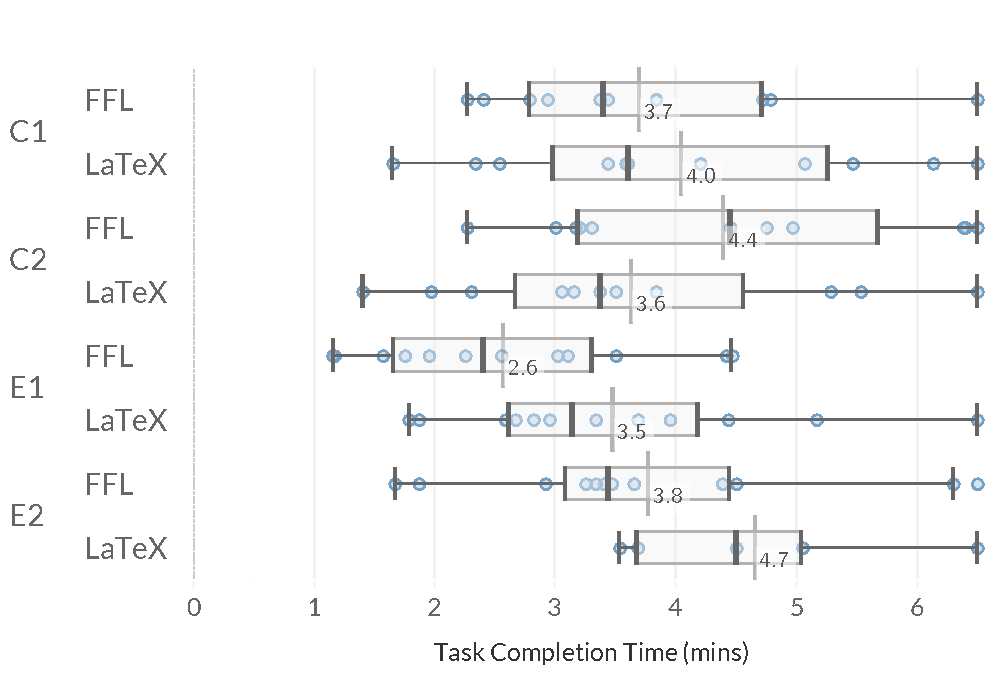
\includegraphics[width=\linewidth]{fig/Timing.pdf}
    \caption{Task completion time. Participants completed tasks E1 \& 2 significantly faster with FFL than with LaTeX. \normalfont Box-and-whiskers depict median, quartiles, and extrema (within 1.5 IQR). An additional, taller vertical line annotates the average. Individual times are rendered as dots in the background. Incompletes are encoded as maximum time. \zed{Per-row mean time and standard deviation appear in \hyperref[tab:speed_table]{Table \ref{tab:speed_table}}.}}
    \Description{Boxplot showing completion times by task and interface. The median completion time is lower with FFL than LaTeX for tasks C1, E1, and E2; and higher for task C2. Tasks C1 and C2 see greater variance in task completion time regardless of interface. For tasks E1 and E2, the median, average, minimum and maximum time are shorter with FFL than LaTeX.}
    \label{fig:timing}
\end{figure}

As depicted in \hyperref[fig:timing]{Figure~\ref{fig:timing}}, participants completed the complex editing tasks (E1 \& E2) more quickly with FFL than with LaTeX. A linear mixed-effects model found the interface to have a significant effect ($F=6.7$, $p=0.02$). Other significant effects include task ($F=11$, $p=2\times10^{-5}$) and task-interface interaction ($F=6.8$, $p=0.001$); task order was not significant. As implied by the task-interface interaction effect, the effect of FFL was stronger for some tasks than others. Fitting the same model to the pairs of creation (C1 \& 2) and editing (E1 \& 2) tasks separately, the effect of FFL was significant for editing tasks ($F = 27$, $p=7\times10^{-5}$), but not for the creation tasks ($p\approx1$). 
\zed{While we note that the test statistics are influenced by our choice to cut off participants at 6.5 minutes, a visual inspection suggests the above trends hold for participants who were not cut off: FFL decreased task time for the 0th--75th quartile participants, none of whom were cut off before completing the task (see Figure~\ref{fig:timing}). Our observations during the study revealed no clear signs that participants were further from completion when cut off in the FFL condition than in the baseline condition.}

\begin{figure}
    \centering
    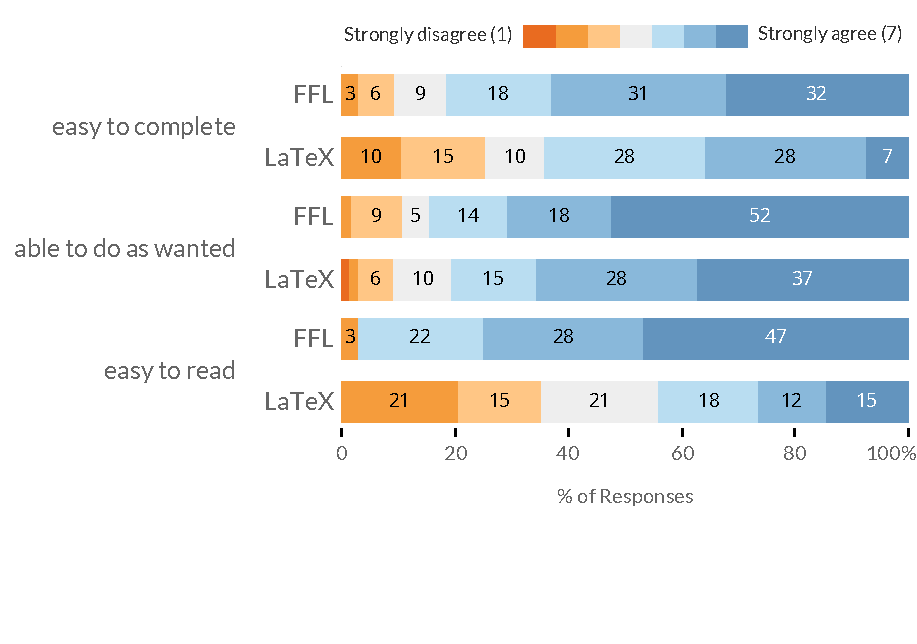
\includegraphics[width=\linewidth]{fig/Responses.pdf}
    \vspace{-2.5em}
    \caption{Self-reported ease for timed tasks. On the whole, participants reported greater ease with FFL than with LaTeX. \normalfont Data comes from responses when participants were asked to indicate agreement (from "strongly disagree" (1) to "strongly agree" (7)) with the statement in the left column of the bar chart. Numbers indicate percentages of total responses relative to the row. \zed{Per-row medians and arithmetic means appear in Tables \ref{tab:ease_table}--\ref{tab:ease_to_read_table}}.}
    \Description{Stacked bar chart of self-reported ease for timed tasks (on a 7-point Likert scale). The three dimensions of ease are “easy to complete”, “able to do as wanted” and “easy to read.” Greater ease is reported with FFL for all three; this difference is slight for “able to do as wanted” and pronounced for “easy to complete” and “easy to read.”}
    \label{fig:responses}
\end{figure}

\subsubsection{Ease}\label{sec:ease}

Participants reported significantly higher ease in completing tasks with FFL than with LaTeX ($F=16$, $p=6\times10^{-4}$). On a 7-point Likert scale, participants reported \zed{a median score of 7, versus 6} with LaTeX (Figure~\ref{fig:responses}). Models fit on subsets of tasks showed the difference in ease to be significant for editing tasks E1 \& 2 ($F=19$, $p=2\times10^{-4}$), but not tasks C1 \& 2 ($p\approx1$).

Additional questions on the questionnaire indicate aspects of FFL that might have led to greater ease. Following the editing tasks E1 \& 2, participants reported significantly greater ease in reading augmentation code (Figure~\ref{fig:responses}) in FFL than with LaTeX ($F=23$, $p=6\times10^{-5}$). In the retrospective questionnaire, participants compared the ease of using FFL to LaTeX for a variety of primitive augmentation operations (Figure~\ref{fig:eos1}), reporting greater ease with FFL for coloring parts of formulas ($W=7$, $p<0.002$, \zed{mdn. 5 vs. 4}), labeling parts of formulas ($W=0$, $p<0.002$, \zed{mdn. 5 vs. 4}), and applying the style to multiple parts of the formulas ($W=24$, $p<0.002$, \zed{mdn. 5 vs. 2}), on a 1--5 scale.

% \begin{center}
\begin{figure}
    \centering
    \vspace{-.5ex}
    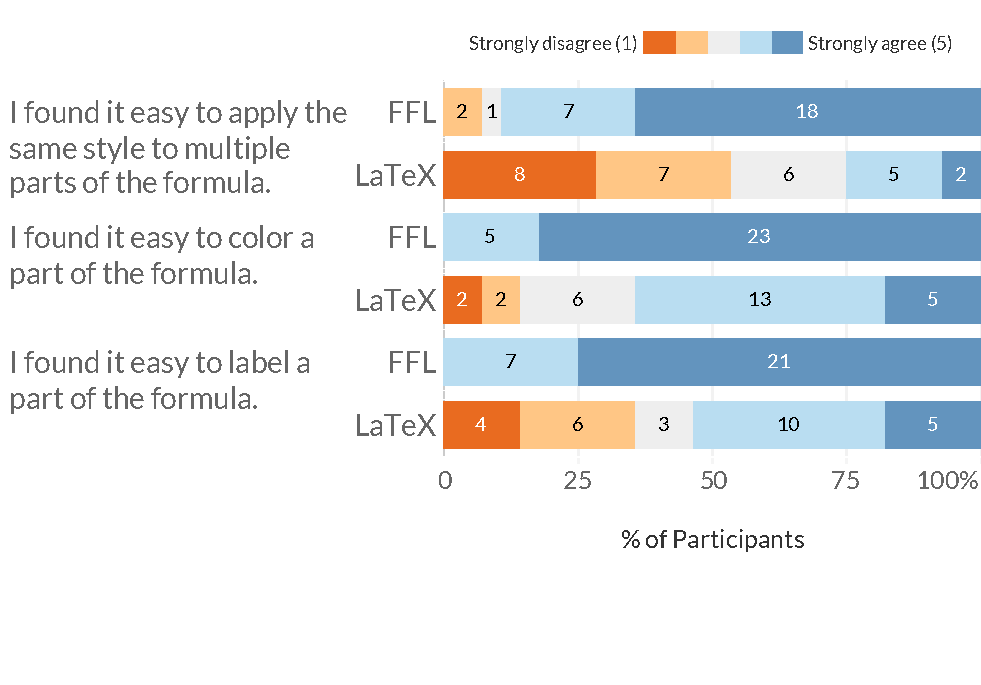
\includegraphics[width=\linewidth]{fig/EOS-1.pdf}
    \vspace{-2.5em}
    \caption{Ease-of-use ratings in retrospective questionnaire. \normalfont Ease was reported on three dimensions for both FFL and LaTeX (shown in the leftmost labels on the bar chart). % \normalfont Participants participants were asked to rate on a scale from "strongly disagree" (1) to "strongly agree" (5) on their agreement with the statement on the left after each task.
    \vspace{-1ex}}\Description{Stacked bar chart of ease-of-use responses in retrospective questionnaire, for three questions asked on a 5-point Likert Scale. The three questions are, “I found it easy to apply the same style to multiple parts of the formula,” “I found it easy to color a part of the formula,” and “I found it easy to label a part of the formula.” A majority of participants “strongly agreed” that FFL made tasks easy in these three ways. Agreement was weaker for LaTeX; with LaTeX, for applying the same style to multiple parts of the formula, 7 / 28 participants reported agreement (either a 4 or 5 out of 5); for coloring a part of the formula, 18 / 28; and for labeling a part of the formula 15 / 28.}
    \label{fig:eos1}
\end{figure}

\subsubsection{Differences in success}

While on the whole participants reported high levels of comfort with LaTeX in the introductory questionnaire, there was still considerable individual variation in comfort with both LaTeX and CSS. When we fit our model to take background factors into account,\footnote{When fitting a model with background factors as fixed effects, we remove the random effect of participant ID.} we observed years of experience of LaTeX as a significant predictor of task speed ($F=10$, $p=5\times10^{-5}$), with interface becoming insignificant ($F=5.4$, $p=.1$). For the creation tasks alone, years of experience with LaTeX is not significant  ($p=.3$). For the editing tasks, years of experience is significant ($F=10$, $p=3\times10^{-4}$), and interface remains a significant effect ($F=27$, $p=6\times10^{-5}$). Other background factors such as self-reported comfort with LaTeX or CSS were not significant predictors. Overall, additional years of experience of LaTeX reduced task completion times, though the trends vary considerably when broken down by task and interface pair.

\subsubsection{Interpretation}

In summary, participants completed tasks about as often with FFL and LaTeX. FFL led to quicker completion, with less difficulty. Post-hoc tests showed the effect to be significant for editing tasks E1 \& 2, but not creation tasks C1 \& 2. We explain this discrepancy with two observations. 

First, E1 \& 2 were performed after C1 \& 2. Some participants reported an initial learning curve with FFL, or encountered gaps or misconceptions regarding FFL during the first pair of tasks. These gaps and misconceptions were sometimes resolved by the time they began the second pair of tasks. Learning effects may provide a partial explanation: among 33 participants, our observation notes showed 23 participants making 35 critical mistakes \zed{(i.e., writing a spec that yielded compilation errors or incorrect outputs)} in C1 \& 2, reduced to 18 participants making 23 mistakes in E1 \& 2.
\zed{Gaps and misconceptions may have also been reduced when participants were given access to starter code in editing tasks E1\&2.}

Second, E1 \& 2 required participants to work with considerably more complex and denser markup along with some augmentation already integrated to begin with. E1 \& 2 reflect a setting where a formula has been augmented and the authors wish to experiment with alternative designs. We interpret this effect to indicate that FFL manifests more value as augmentation markup becomes larger; in the LaTeX baseline, this results in the markup languages becoming increasingly tangled and difficult to evolve, as discussed in greater detail in the next section.

\subsection{Effect of FFL on authoring experience}

In this section, we review observations, interviews, and questionnaire data to arrive at a comprehensive understanding of how FFL supports, and in some cases works against, the experience of formula augmentation. Overall, participants found FFL's ``core'' features useful (Figure~\ref{fig:features_use}). This section introduces strengths and shortcomings of FFL in terms of the cognitive dimensions of notation~\cite{ref:blackwell2003notational}, a framework used in programming language design to \zed{examine and discuss} the effect of language design choices.

\begin{figure}
    \centering
    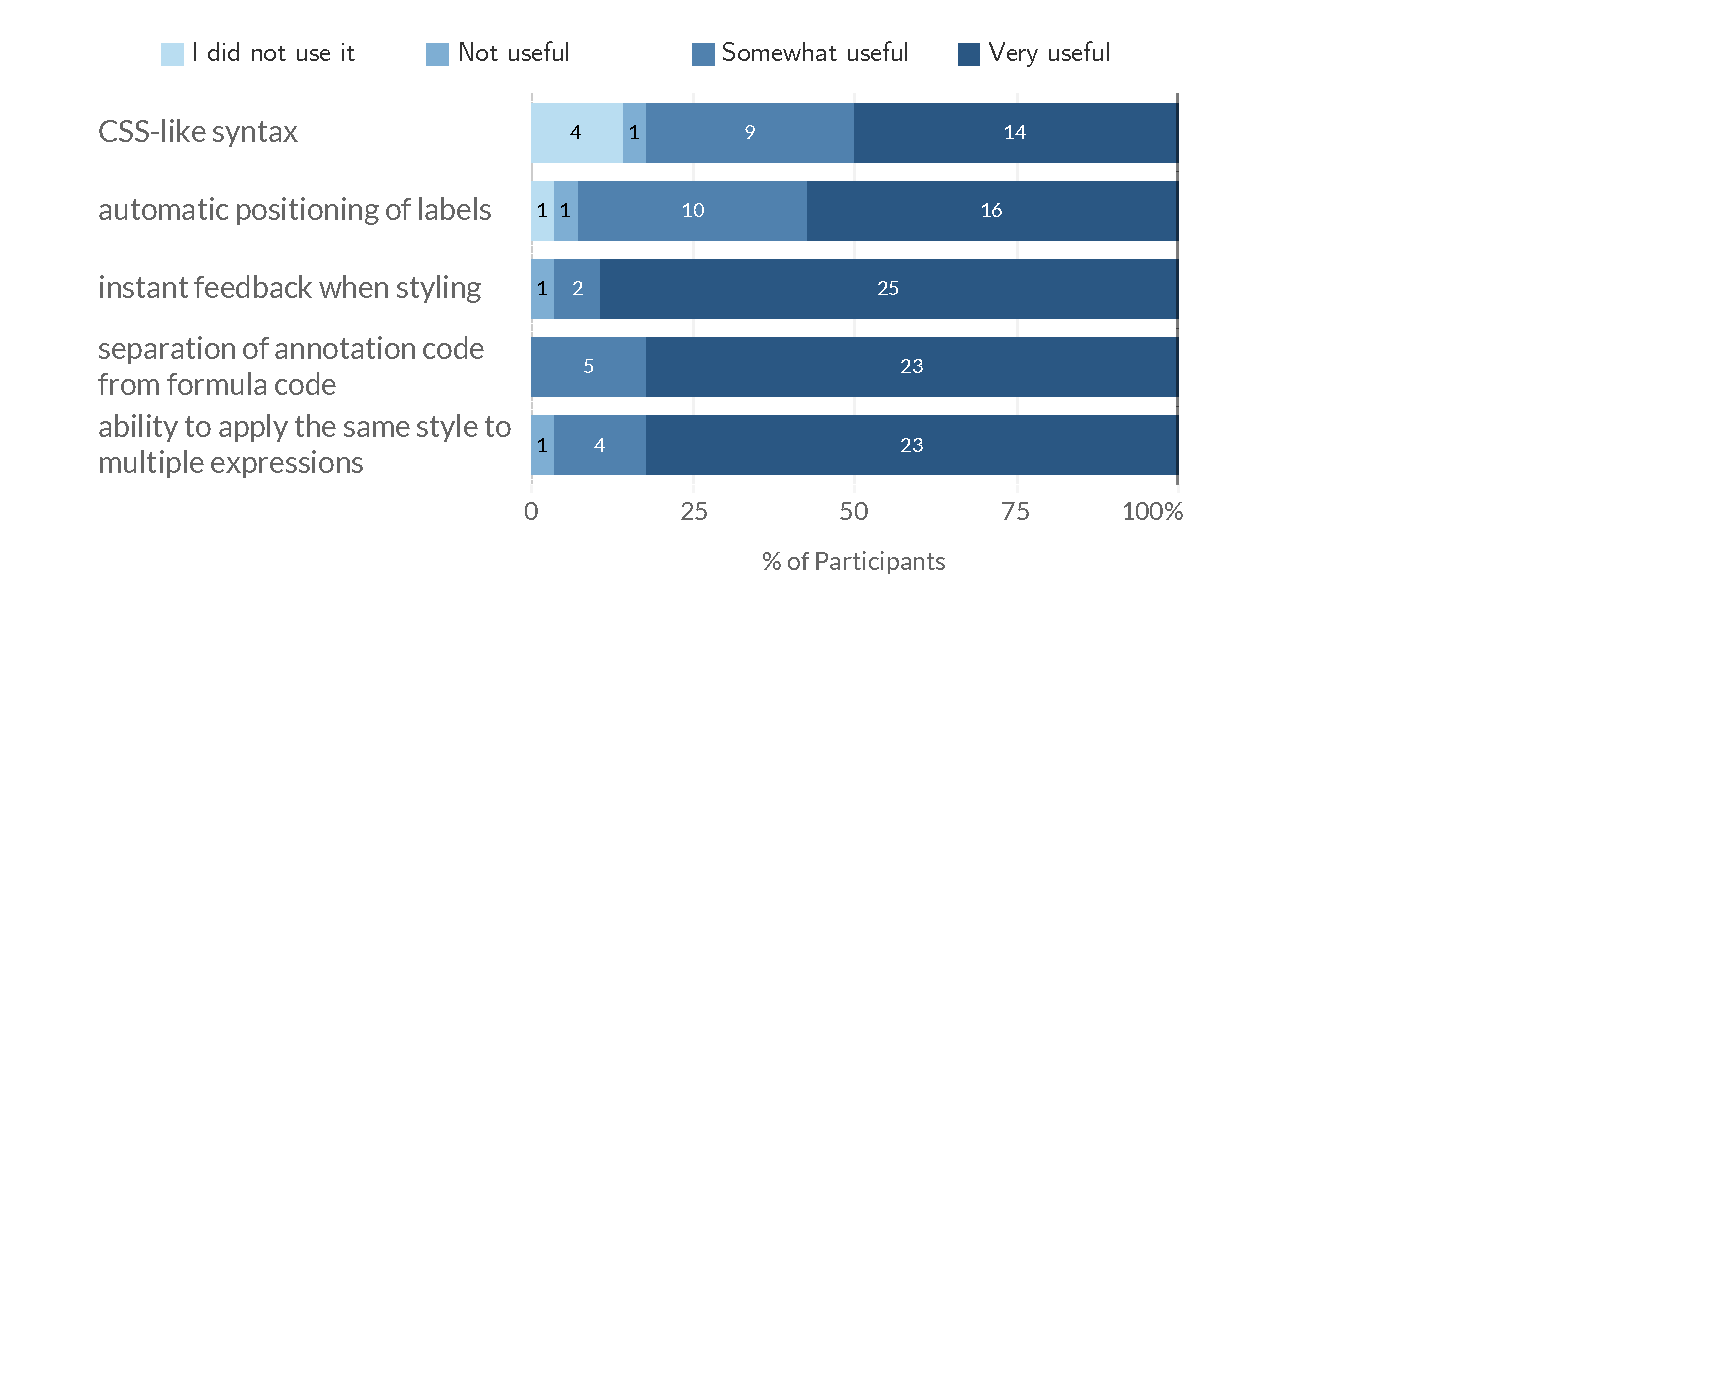
\includegraphics[width=\linewidth]{fig/Useful.pdf}
    \vspace{-3ex}
    \Description{Stacked bar chart of usefulness of 5 features (on a 4-point scale, including “I did not use it,” “not useful,” “somewhat useful,” and “very useful”). The five features are “CSS-like syntax,” “automatic positioning of labels,” “instant feedback when styling,” “separation of annotation code from formula code,” and “the ability to apply the same style to multiple expressions.” For all features except for “CSS-like syntax,” a majority of participants reported “very useful.” The vast majority of participants found “instant feedback,” “separation of annotation code from formula code,” and “the ability to apply the same style to multiple expressions” very useful. 14/28 participants found CSS-like syntax very useful, and 9/28 participants found it somewhat useful.}
    \caption{Usefulness of features. \normalfont Shown are participants' responses to the question ``How useful was \emph{[feature]} when you used FFL to augment math formulae?''
    }
    \label{fig:features_use}
\end{figure}

\subsubsection{Strengths} FFL improved the authoring experience as follows:

\paragraph{Viscosity}
FFL reduced the number of actions required to accomplish some goals. This was most clear when participants edited augmentations for multiple expressions at once. Participants frequently expressed appreciation for the ability to make cross-cutting changes with a single style specification (5), and wished for a similar capability for LaTeX (4). Making cross-cutting changes was described as more ``efficient'' (P4) and ``easier'' (P12, P24) with FFL. \zed{All but one} participant described the ability to apply one style to multiple expressions as very useful (Figure~\ref{fig:features_use}).

\paragraph{Hard mental operations}

FFL made it easier for participants to orient themselves to augmentation markup. LaTeX was the less preferred choice for reading markup (Figure~\ref{fig:responses}). LaTeX was described as difficult to read (16) and used complex or unintuitive syntax (6). The association of augmentations with expressions is difficult to understand due to the dependence on copious numbers of nested braces to associate them (14). Reading LaTeX was therefore described as ``holding a lot of moving pieces in my mind'' (P18), where ``it is a nightmare to look for what I am editing'' (P13). Reading challenges arose when participants had difficulty identifying expressions to which LaTeX commands applied (2), mapping from parts of the rendered formula to the corresponding LaTeX (5), reading and editing the markup (3), and pinpointing sources of errors (2).

In comparison, FFL seemed easier to read---we rarely heard similar criticisms levied against FFL. 16 participants explicitly mentioned their appreciation for the separation of formula markup from augmentation markup; this division was called a ``big advantage'' and ``very powerful'' (P13). The separation of annotation code from formula code was reported as ``very useful'' by the vast majority of participants in the retrospective questionnaire, and ``somewhat useful'' by all remaining participants. Participants rated the readability of FFL significantly higher than LaTeX (Section~\ref{sec:ease}).

\paragraph{Error proneness}

FFL removed a class of errors with its approach to associating expressions with augmentations. As mentioned in prior work~\cite{ref:head2022math}, one challenge of using LaTeX to augment formulas is to use braces correctly to associate augmentations with expressions. Participants described braces as ``annoying'' (P28), finding it difficult to find matching pairs of braces (6), and desiring the ability to find out which braces are redundant or missing (2). Braces were the most common kind of error we observed: at least some participants made a bracing error for each task (8 participants for task C1; 2 for C2; 6 for E1; and 8 for E2). Participants also encountered issues with using \texttt{\textbackslash{}def} correctly, writing arguments to commands in the right order, and other LaTeX compilation errors. As noted by participants, FFL did not see these difficulties due to its approach to associating augmentations with expressions (2).

\paragraph{Closeness of mapping}

In several situations, FFL provided a close mapping to the ways participants could envision expressing augmentations. Two participants described that the metaphor of CSS, including its use of selectors and attributes, was ``intuitive.'' The design of selectors allowed participants to indicate which expressions they wished to augment by selecting, and then copying and pasting, those expressions from the formula into their FFL specification (2). When asked to indicate the degree to which FFL ``did what I expected to,'' all but 2 participants agreed, and over half of the participants strongly agreed.

On the whole, participants developed comfort with a large number of primitives in a short amount of time. By the time they performed the exploratory authoring task, participants had developed enough comfort with the language that they frequently made use of color (24), labels with leader lines (19), and labels with extent markers (11). These augmentations made use of myriad language features, including single-character wildcards (15), sequence wildcards (15), unions (11), and the adjustment of label positions (9). See Appendix Section~\ref{sec: open_task_image} for examples.

\paragraph{Progressive evaluation}

The favorite feature of FFL was the instant feedback supported by the FFL runtime. More participants described this feature as ``very useful'' than any other feature. 7 participants explicitly indicated their appreciation for instant feedback. In contrast, the LaTeX toolset required slower compilation of the document to see the effect of one's changes to the markup (2), which was described as ``not very convenient'' (P21).

\subsubsection{Shortcomings}\label{sec:shortcomings} While FFL improved the experience of authoring formulas in numerous ways, it also introduced new challenges meriting new solutions to design and training:

\paragraph{Closeness of mapping}
FFL was not without a learning curve. Some participants found aspects of the CSS-like syntax challenging (8); this is in part because participants generally had low self-reported comfort with CSS (Section \ref{study-participants}). Participants also expressed discomfort with the \texttt{glob} syntax~\cite{UnixMan} for wildcards (1), and other aspects of LaTeX's math mode (5). These experiences serve as a reminder that FFL expects familiarity with CSS, glob, and LaTeX. We expect many authors seeking to use FFL in web documents would have this experience; though FFL still imposes a threshold to entry. An additional indicator of a learning curve is that 8 participants reviewed the cheat sheet before beginning their first task with FFL, suggesting that the tutorial was not enough to internalize the syntax. Similar challenges were observed for the LaTeX baseline, with participants forgetting commands taught in the tutorial (3) or failing to properly use commands from the cheat sheet (3).

While participants largely succeeded in selecting expressions with the selector syntax, several participants desired support for direct selection through mouse interaction with the formula (3). Similarly, participants desired the ability to highlight expressions corresponding to a selector (3). Participants also desired code generation (1) and no-code features (2), where style code could be partially or completely generated for the author. Direct selection features are beyond the scope of a language design, though they might serve as useful additions to an editing environment.

\paragraph{Error proneness}

FFL removed some classes of errors, though they introduced friction for others. The current runtime provides only very limited support for error tolerance, reporting, and recovery. 6 participants introduced typos and had difficulty understanding why their augmentation markup was not working as intended when they failed to notice those typos.
Some of these typos arose from challenges related to ``closeness of mapping''---several participants used incorrect delimiters that perhaps best reflected a lack of familiarity with the base CSS syntax. 3 participants wished that FFL continued to render live even when errors were present in the markup. For these reasons, participants desired numerous standard editor affordances that assist in reducing errors, including autocomplete (7), syntax highlighting (2), and templates (3).

\paragraph{Visibility}
Any sufficiently complex language contains constructs users are unaware of. We observed several such constructs for FFL that were either undiscoverable or poorly suited once discovered.

First, participants expressed confusion around scoping augmentations. The default behavior of the FFL runtime is to apply selectors globally across an entire document. What should an author do when they wish for their augmentation rules to apply to only a single expression, formula, or single passage? Several authors had this specific question (8). The current solutions in FFL are (1) the \texttt{intersect} command; (2) an \texttt{:nth} selector that selects an indexed occurrence; (3) creating an indexable group in the formula markup by adding brackets around it; (4) using style overriding (i.e., using one rule to style all expressions, and a second rule to revert it for some subset of those expressions). These features were largely unused, perhaps due to issues of discoverability or learnability. At least 2 participants expressed some confusion with overriding.

Second, participants desired more influence over the appearance of labels, including label size (4), color (3), and font-weight (3). While the \texttt{.ffl-label} class is applied to all labels for just this purpose, participants were not often aware of it. These undiscovered features represent opportunities to either increase visibility or redesign constructs to be easier to guess.

\paragraph{Expressiveness}
Expressiveness is not a cognitive dimension of notation, though we discuss it here as a catchall for controls participants desired that FFL did not provide. One often-desired feature was the ability to assign a single label to multiple expressions simultaneously. For example, in the exploratory task, participants often wanted to create one label for ``slope'' and connect it via leader lines to all four $\beta$ terms in the formula (9). The default behavior of FFL is to assign a label to only the first matched expression in a formula. As one participant noted, this made the behavior of FFL inconsistent, because style rules applied to all matching expressions, while labels applied to only the first matched expression (P23). Several participants wished for different behavior from the automatic label layout algorithm (4), and desired the ability to fine-tune label layout beyond FFL's current capabilities (3).

\section{Discussion}

Our study showed greater speed, ease, and readability of markup code with FFL for the second pair of tasks, which were complex editing tasks. Evidence from the study suggests FFL reduces viscosity, hard mental operations, and error proneness, while providing affordances promoting closeness of mapping and progressive evaluation. These findings suggest the promise of the ideas behind FFL, namely the separation of formula and augmentation markup, live feedback, and its approach to syntax. In this section, we examine the generalizability of the findings and opportunities for advancing the research agenda of which FFL is a part.

\subsection{Limitations}

The generalizability of our findings is necessarily limited to tasks and the sample of participants we studied. When interpreting the results, it is useful to take stock of how authors of web-based math documents would differ from participants in the study.

First, \zed{we anticipate that real-world authors would have greater motivation to use the tools. If an author chose to use FFL, it would reflect a desire to make notation more approachable. We expect a real-world author might therefore experiment more ambitiously with the tools compared to study participants who may not have had prior experience explaining formulas in their writing.}

Second, they would likely be familiar with the formula markup, having written it themselves: for both the LaTeX and FFL conditions, this would likely lead to faster task completion times.

Third, users ``in the wild'' would not have the luxury of having the tools demonstrated over a 10-minute tutorial, and therefore may have more difficulty in a walk-up-and-use experience.

And finally, their FFL markup would have likely gotten longer if they were augmenting a full-length document.
\zed{Our lab study only assigned single-formula tasks because it made it possible for us to select pairs of real-world augmentations where each member of the pair was of approximately equal complexity. Some tasks did require making cross-cutting changes.}
That said, participants in our study did not get a chance to encounter complexities that might arise with longer style specifications, and we did not observe all the difficulties to be seen with scoping augmentation.

Of these limitations, the fourth and fifth are indicators that our lab study reveals only a subset of challenges using FFL; the remaining limitations suggest that task performance could improve for FFL, or both FFL and LaTeX, in more realistic settings. Challenges to using FFL should be further documented by refining the FFL toolkit and evaluating its use in real authoring settings.

\subsection{Future work}

A first line of future research should address opportunities in extending FFL, some already revealed in the study (Section~\ref{sec:shortcomings}).

\paragraph{Scoping} Authors necessarily wish to restrict augmentations to particular expressions, formulas, and passages. While the FFL language provides such capabilities, these were either not discovered or used ineffectively by participants. A future solution could be to let authors specify local ``scopes'' of application in the document markup (e.g., labeling individual passages or formulas) in order to refer to them in selectors.

\paragraph{Resilient expression matching} FFL's current approach to matching token sequences leads to some brittleness in matching expressions that are rendered the same way, but have different LaTeX markup (e.g., in the current implementation, \texttt{\$a\_0\textasciicircum{}1\$} matches ``\texttt{\$a\_0\textasciicircum{}1\$}'' but not ``\texttt{\$a\textasciicircum{}1\_0\$},'' even though they are rendered identically). This was largely not a problem for participants in the study, though we find this undesirable in our own use. FFL provides some flexibility to address cases like these, but we believe a more robust implementation of FFL may benefit from matching patterns with abstract syntax trees, rather than concrete token sequences.

\paragraph{Further improvements} 
As noted in Section~\ref{sec:shortcomings}, FFL should be extended with the ability to apply one label to multiple expressions, more precisely adjust the positions of labels, and better recognize and recover from syntax errors.

\vspace{2.5ex}

This research also points the way to follow-up research on math augmentation that extends into new sorts of tooling.

\paragraph{Direct augmentation}
Some participants desired assistance in writing selectors, understanding selections, and expressing styles. They proposed the ability to directly select them, highlight rendered expressions that are matched by selectors, and generate styles (Section~\ref{sec:shortcomings}). We see FFL as a stepping stone to interactive authoring tools involving direct augmentation like those described by participants, where FFL is used as a substrate, similarly to how backend visualization grammars like Vega-Lite~\cite{ref:satyanarayan2017vegalite} enables visualization exploration interfaces like Voyager~\cite{ref:wongsuphasawat2015voyager}. 

\paragraph{Animated formulas}
FFL was designed to augment static texts, like blog articles or online textbooks. What would an augmentation language look like for dynamic presentations of notation, like animations on the popular \emph{3Blue1Brown}~\cite{ref:3Blue1Brown} YouTube channel for explaining math, where formulas are built up step-by-step and annotated gradually with color and labels? We see FFL as a starting point for developing grammars of animated notation. However, new primitives would have to be designed, as they have in other areas with generalized visualization annotation DSLs for animation~\cite{ref:ge2020canis}.

\paragraph{Making texts interactive}
One pattern of augmentation is creating interactive formulas, where readers can tinker with the values of expressions and see how it influences downstream computations in the formula~\cite{ref:head2022math}.
Prior tools like Idyll~\cite{ref:conlen2018idyll}, \emph{Tangle.js}~\cite{tool:victortangle}, and Potluck~\cite{ref:litt2022potluck} envision the creation of parametric documents where values update reactively as users interact with controls. Extensions to FFL could unify such affordances with its syntax, perhaps even taking advantage of the computation a formula represents to automatically map values in one part of a formula to values elsewhere.

\paragraph{Accessibility}
Augmentations specified in a language like FFL encode additional meaning about a formula, such as what symbols make up meaningful expressions, and what those expressions mean. This information should ideally be surfaced in a way that is accessible to blind and low-vision readers. FFL could be extended to provide cues to screen readers to read a formula aloud in ways that improve upon the default reading order.
\section{Conclusion}

\zed{Our controlled lab study yielded two results. First, in complex editing tasks, FFL led to faster and easier editing of augmentation markup compared to a LaTeX baseline, while yielding more readable markup. Second, for simpler tasks where authors wrote simple augmentations from scratch, we observed no significant differences between FFL and the baseline.}
Our study offers signs that FFL reduces viscosity, hard mental operations, and error proneness, while supporting closeness of mapping and progressive evaluation. This paper demonstrates the potential of tools like FFL that extend authoring environments to support the practice of augmenting notation. We hope tools like FFL bring about more pervasive authoring of approachable explanations of math notation.


\begin{acks}
We thank authors who graciously published articles with augmented formulas which we adapted as demo material and study stimuli \cite[Mohammed et al., Murad, Azad, Cockett \& Heagy, Hohman et al.]{mohammed2020continuous,ref:murad2020navierstokes,W4,ref:cockett2016pixels,ref:hohman2019gamut}, Dr. Rowan Cockett for sharing with us his experience in scientific communication and document editing tools, members and friends of \textit{Penn HCI} for providing early feedback on the tool and the study, as well as open-source contributors who not only created the libraries and tools which we directly cited, but also many indirect dependencies that make what we do possible.
\end{acks}

\bibliographystyle{ACM-Reference-Format}
\bibliography{refs,andrew-base,andrew-extras}

\appendix
\section{Descriptive statistics}\label{sec: result_table}

\setcounter{figure}{0}    
\setcounter{table}{0}
\renewcommand\thetable{\thesection.\arabic{table}}  
\renewcommand\thefigure{\thesection.\arabic{figure}}  

Below, we show detailed tables and figures of descriptive statistics collected from the usability study.

\subsection*{Task completion}

\aptLtoX[graphic=no,type=html]{  \begin{table}[H]
    \centering
    \begin{tabular}[t]{l|r r r r}
        & Task C1 & Task C2 & Task E1 & Task E2 \\\hline
        \textit{FFL}     &3&2&0&1\\
        \LaTeX  &2&1&1&8
    \end{tabular}
    \Description{Table. Each row corresponds to an interface, and each column corresponds to a task that was completed with that interface. Cells contain counts of participants who completed the task with that interface.}
    \vspace{1ex}
    \captionof{table}{Counts of participants who did not complete timed tasks (each count is out of 14 participants).}
    \label{tab:count_fail_task}
 \end{table} }{ % \begin{table}[H]
\begin{center}
    \centering
    \begin{tabular}[t]{l|r r r r}
        & Task C1 & Task C2 & Task E1 & Task E2 \\\hline
        \textit{FFL}     &3&2&0&1\\
        \LaTeX  &2&1&1&8
    \end{tabular}
    \Description{Table. Each row corresponds to an interface, and each column corresponds to a task that was completed with that interface. Cells contain counts of participants who completed the task with that interface.}
    \vspace{1ex}
    \captionof{table}{Counts of participants who did not complete timed tasks (each count is out of 14 participants).}
    \label{tab:count_fail_task}
\end{center}
% \end{table}
 } 


\aptLtoX[graphic=no,type=html]{ \begin{table}[H]
    % \centering
    \resizebox{\linewidth}{!}{
        \begin{tabularx}{1.07\linewidth}{X|c c c c c c c c}
            Time&\multicolumn{2}{c}{Task C1}&\multicolumn{2}{c}{Task C2}&\multicolumn{2}{c}{Task E1}&\multicolumn{2}{c}{Task E2} \\
            (s)&\textit{FFL}&\LaTeX&\textit{FFL}&\LaTeX&\textit{FFL}&\LaTeX&\textit{FFL}&\LaTeX \\\hline
            $\bar{x}$&253.3&242.8&258.1&229.2&157.3&206.0&223.4&350.4\\
            $\sigma$&97.65&101.1&98.6&95.8&66.4&81.3&87.5&68.1
        \end{tabularx}
    }\Description{Table of task completion times, in seconds, by interface-task pair (measured in seconds). Task C1 with FFL, mean: 253.3, standard deviation: 97.65; with LaTeX, mean: 242.8, standard deviation: 101.1. Task C2, with FFL, mean: 258.1, standard deviation: 98.6; with LaTeX, mean: 229.2, standard deviation: 95.8; Task E1, with FFL, mean: 157.3, standard deviation: 66.4; with LaTeX, mean: 206.0, standard deviation: 81.3. Task E2, with FFL, mean: 223.4, standard deviation: 87.5; with LaTeX, mean: 350.4, standard deviation: 68.1.}
    \vspace{1ex}
    \captionof{table}{Task completion times, reported as arithmetic means and standard deviations, by task and interface.}
    \label{tab:speed_table}
 \end{table}
 }{ % \begin{table}[H]
\begin{center}
    % \centering
    \resizebox{\linewidth}{!}{
        \begin{tabularx}{1.07\linewidth}{X|c c c c c c c c}
            Time&\multicolumn{2}{c}{Task C1}&\multicolumn{2}{c}{Task C2}&\multicolumn{2}{c}{Task E1}&\multicolumn{2}{c}{Task E2} \\
            (s)&\textit{FFL}&\LaTeX&\textit{FFL}&\LaTeX&\textit{FFL}&\LaTeX&\textit{FFL}&\LaTeX \\\hline
            $\bar{x}$&253.3&242.8&258.1&229.2&157.3&206.0&223.4&350.4\\
            $\sigma$&97.65&101.1&98.6&95.8&66.4&81.3&87.5&68.1
        \end{tabularx}
    }\Description{Table of task completion times, in seconds, by interface-task pair (measured in seconds). Task C1 with FFL, mean: 253.3, standard deviation: 97.65; with LaTeX, mean: 242.8, standard deviation: 101.1. Task C2, with FFL, mean: 258.1, standard deviation: 98.6; with LaTeX, mean: 229.2, standard deviation: 95.8; Task E1, with FFL, mean: 157.3, standard deviation: 66.4; with LaTeX, mean: 206.0, standard deviation: 81.3. Task E2, with FFL, mean: 223.4, standard deviation: 87.5; with LaTeX, mean: 350.4, standard deviation: 68.1.}
    \vspace{1ex}
    \captionof{table}{Task completion times, reported as arithmetic means and standard deviations, by task and interface.}
    \label{tab:speed_table}
% \end{table}
\end{center} } 


\subsection*{Self-reported ease}

In the tables below, cells show the mean \zed{and median} rating across participants on a Likert scale of 1--7, where 1 corresponds to ``strongly disagree'' and 7 corresponds to ``strongly agree'' to a statement.

\aptLtoX[graphic=no,type=html]{ 
 \begin{table}[H]
    % \centering
    \resizebox{\linewidth}{!}{
        \begin{tabular}{l|r r r r r}
            Avg./\zed{Mdn.} Score (1-7) & Task C1 & Task C2 & Task E1 & Task E2 & Exp. Task \\\hline
            \textit{FFL}     &5.47/6.0&5.31/5.5&6.38/6.5&5.44/5.5&6.30/6.0\\
            \LaTeX  &5.00/5.0&5.24/5.0&5.13/6.0&3.61/3.5&N/A
        \end{tabular}
    }\Description{Table. Each row corresponds to an interface; each column to a task. Cells contain the average score of participants’ self-reported ease for using the interface for the task.}
    \vspace{1ex}
    \captionof{table}{Participants' self-reported ease by task and interface. \normalfont Participants were asked to indicate their agreement with the statement ``It was easy to complete the task.''}
    \label{tab:ease_table}
 \end{table}
 }{ \begin{center}
% \begin{table}[H]
    % \centering
    \resizebox{\linewidth}{!}{
        \begin{tabular}{l|r r r r r}
            Avg./\zed{Mdn.} Score (1-7) & Task C1 & Task C2 & Task E1 & Task E2 & Exp. Task \\\hline
            \textit{FFL}     &5.47/6.0&5.31/5.5&6.38/6.5&5.44/5.5&6.30/6.0\\
            \LaTeX  &5.00/5.0&5.24/5.0&5.13/6.0&3.61/3.5&N/A
        \end{tabular}
    }\Description{Table. Each row corresponds to an interface; each column to a task. Cells contain the average score of participants’ self-reported ease for using the interface for the task.}
    \vspace{1ex}
    \captionof{table}{Participants' self-reported ease by task and interface. \normalfont Participants were asked to indicate their agreement with the statement ``It was easy to complete the task.''}
    \label{tab:ease_table}
% \end{table}
\end{center} } 


\aptLtoX[graphic=no,type=html]{ 
 \begin{table}[H]
    % \centering
    \resizebox{\linewidth}{!}{
        \begin{tabular}{l|r r r r r}
            Avg./\zed{Mdn.} Score (1-7) & Task C1 & Task C2 & Task E1 & Task E2 & Exp. Task \\\hline
            \textit{FFL}     &6.06/7.0&5.69/6.5&6.63/7.0&5.44/5.5&6.30/7.0\\
            \LaTeX  &6.00/6.0&6.29/7.0&5.86/6.0&4.72/5.0&N/A
        \end{tabular}
    }\Description{Table. Each row corresponds to an interface; each column to a task. Cells contain the average score of participants’ self-reported efficacy from using the interface for the task.}
    \vspace{1ex}
    \captionof{table}{Participant self-reported efficacy by task and interface. \normalfont Participants were asked to indicate their agreement with the statement ``I was able to do what I wanted with the tool.''}
    \label{tab:was_able_table}
 \end{table}
  }{ \begin{center}
% \begin{table}[H]
    % \centering
    \resizebox{\linewidth}{!}{
        \begin{tabular}{l|r r r r r}
            Avg./\zed{Mdn.} Score (1-7) & Task C1 & Task C2 & Task E1 & Task E2 & Exp. Task \\\hline
            \textit{FFL}     &6.06/7.0&5.69/6.5&6.63/7.0&5.44/5.5&6.30/7.0\\
            \LaTeX  &6.00/6.0&6.29/7.0&5.86/6.0&4.72/5.0&N/A
        \end{tabular}
    }\Description{Table. Each row corresponds to an interface; each column to a task. Cells contain the average score of participants’ self-reported efficacy from using the interface for the task.}
    \vspace{1ex}
    \captionof{table}{Participant self-reported efficacy by task and interface. \normalfont Participants were asked to indicate their agreement with the statement ``I was able to do what I wanted with the tool.''}
    \label{tab:was_able_table}
% \end{table}
\end{center} } 


\aptLtoX[graphic=no,type=html]{ 
 \begin{table}[H]
    % \centering
        \begin{tabular}{l|r r r r r}
            Avg./\zed{Mdn.} Score (1-7) & Task E1 & Task E2 \\\hline
            \textit{FFL}     &6.25/6.0&6.00/6.5\\
            \LaTeX  &5.06/5.0&3.61/3.0
        \end{tabular}
    \Description{Table. Each row corresponds to an interface; each column to a task. Cells contain the average score of participants’ self-reported sense of readability of style code when using the interface for the task.}
    \vspace{1ex}
    \captionof{table}{Participant self-reported sense of readability. \normalfont Participants were asked to indicate their agreement with the statement ``I found it easy to read the styling code/specification.''}
    \label{tab:ease_to_read_table}
 \end{table}
  }{ \begin{center}
% \begin{table}[H]
    % \centering
        \begin{tabular}{l|r r r r r}
            Avg./\zed{Mdn.} Score (1-7) & Task E1 & Task E2 \\\hline
            \textit{FFL}     &6.25/6.0&6.00/6.5\\
            \LaTeX  &5.06/5.0&3.61/3.0
        \end{tabular}
    \Description{Table. Each row corresponds to an interface; each column to a task. Cells contain the average score of participants’ self-reported sense of readability of style code when using the interface for the task.}
    \vspace{1ex}
    \captionof{table}{Participant self-reported sense of readability. \normalfont Participants were asked to indicate their agreement with the statement ``I found it easy to read the styling code/specification.''}
    \label{tab:ease_to_read_table}
% \end{table}
\end{center} } 


\section{Example Augmentations}\label{sec: open_task_image}
Below, we show examples of augmentations authors performed in the open-ended authoring task on again \cite[Hohman et al.]{ref:hohman2019gamut}. The following passage from P26 is representative of most participants' finished work. It makes use of color to relate expressions to descriptions in the text, and labels to explain several expressions. \\[1ex]

\centerline{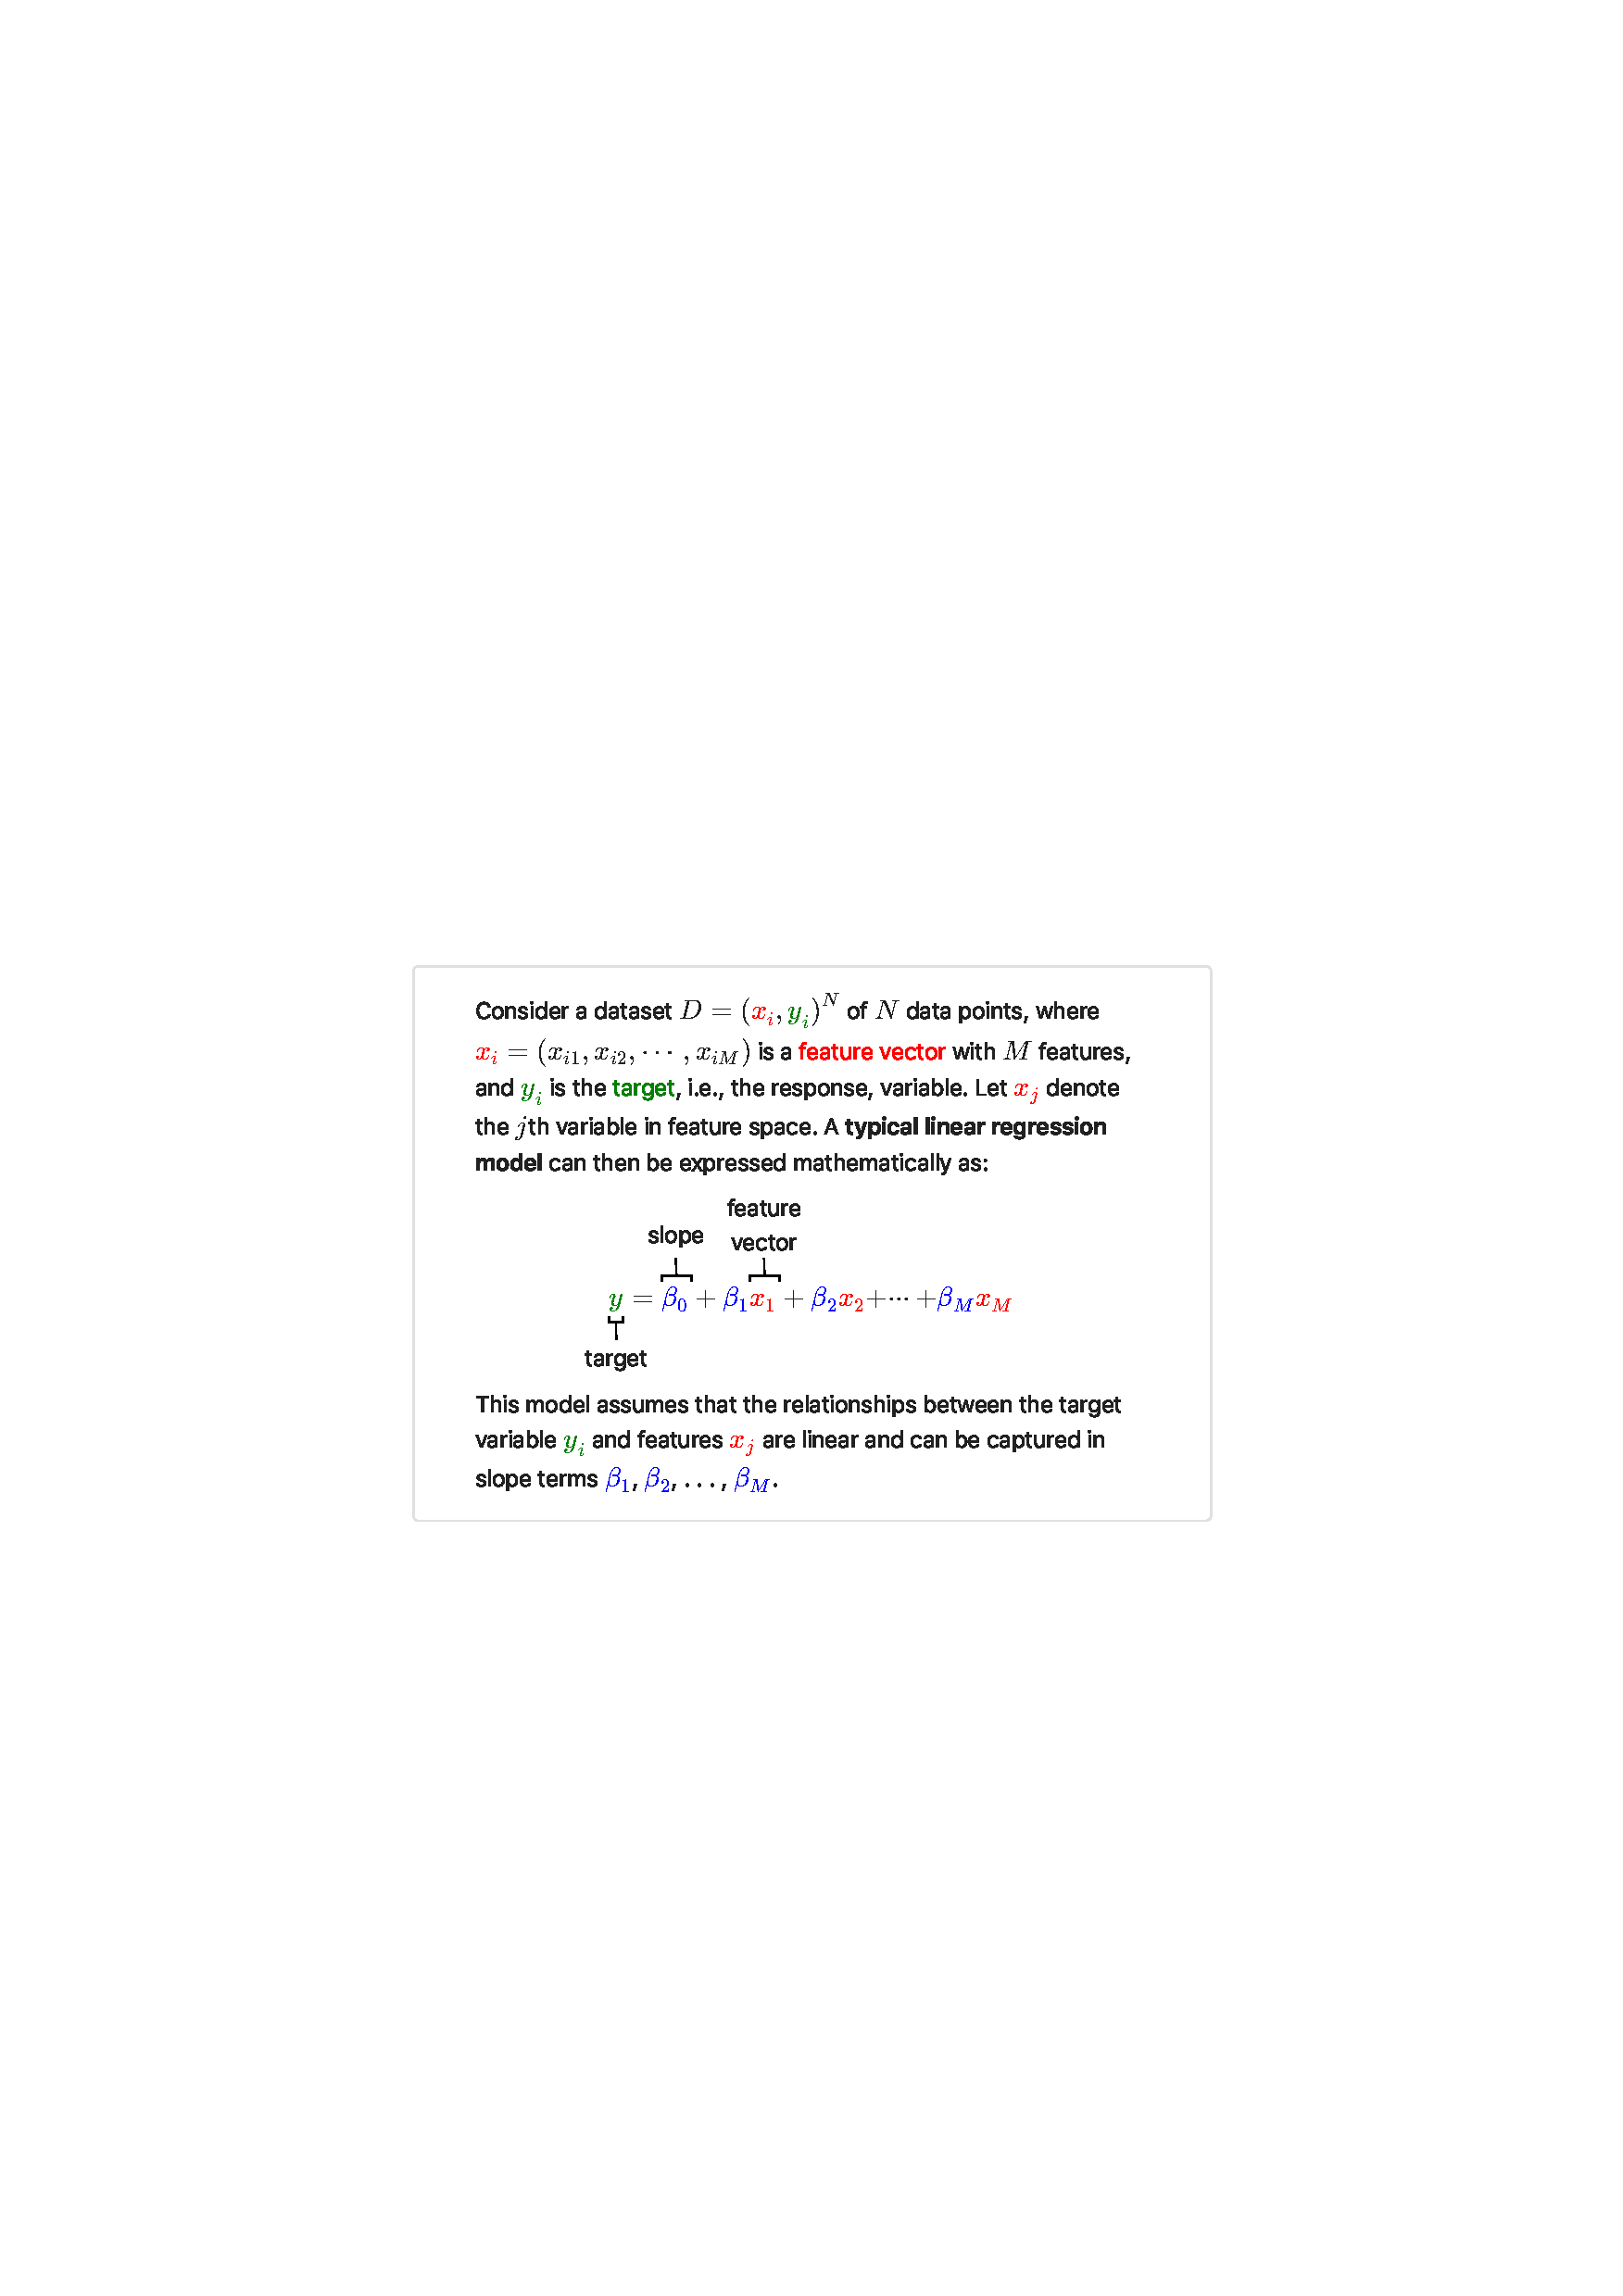
\includegraphics[width=.86\linewidth]{figures/o-2595}\Description{An example augmentation authored by P26 in the exploratory task. All appearances of “x” and “x” with subscripts are colored red, as is the phrase explaining that “x” is a feature vector. All appearances of “y” and “y” with subscripts are colored green, as is the phrase explaining that “y” is the “target” variable. All appearances of “beta” with subscripts are colored in blue. In the block formula, “y” is labeled “target,” “beta-sub-0” is labeled “slope,” and “x-sub-1” is labeled “feature vector,” all with extent markers.}}

% The above was a typical augmentation by P26. To enhance the readability of the given maths excerpt, P26 used various colors to draw associations between formula terms and related text, and labels to explain terms in the formula. 

Other participants took different approaches. For instance, P13 used labels alone, believing them to be sufficient for a textbook-style passage (and that color was better suited for personal notes):\\[1ex]
% We observed that participants' styling preferences varied. Some participants preferred only adding labels but not any colors. For example,\\
{\centerline{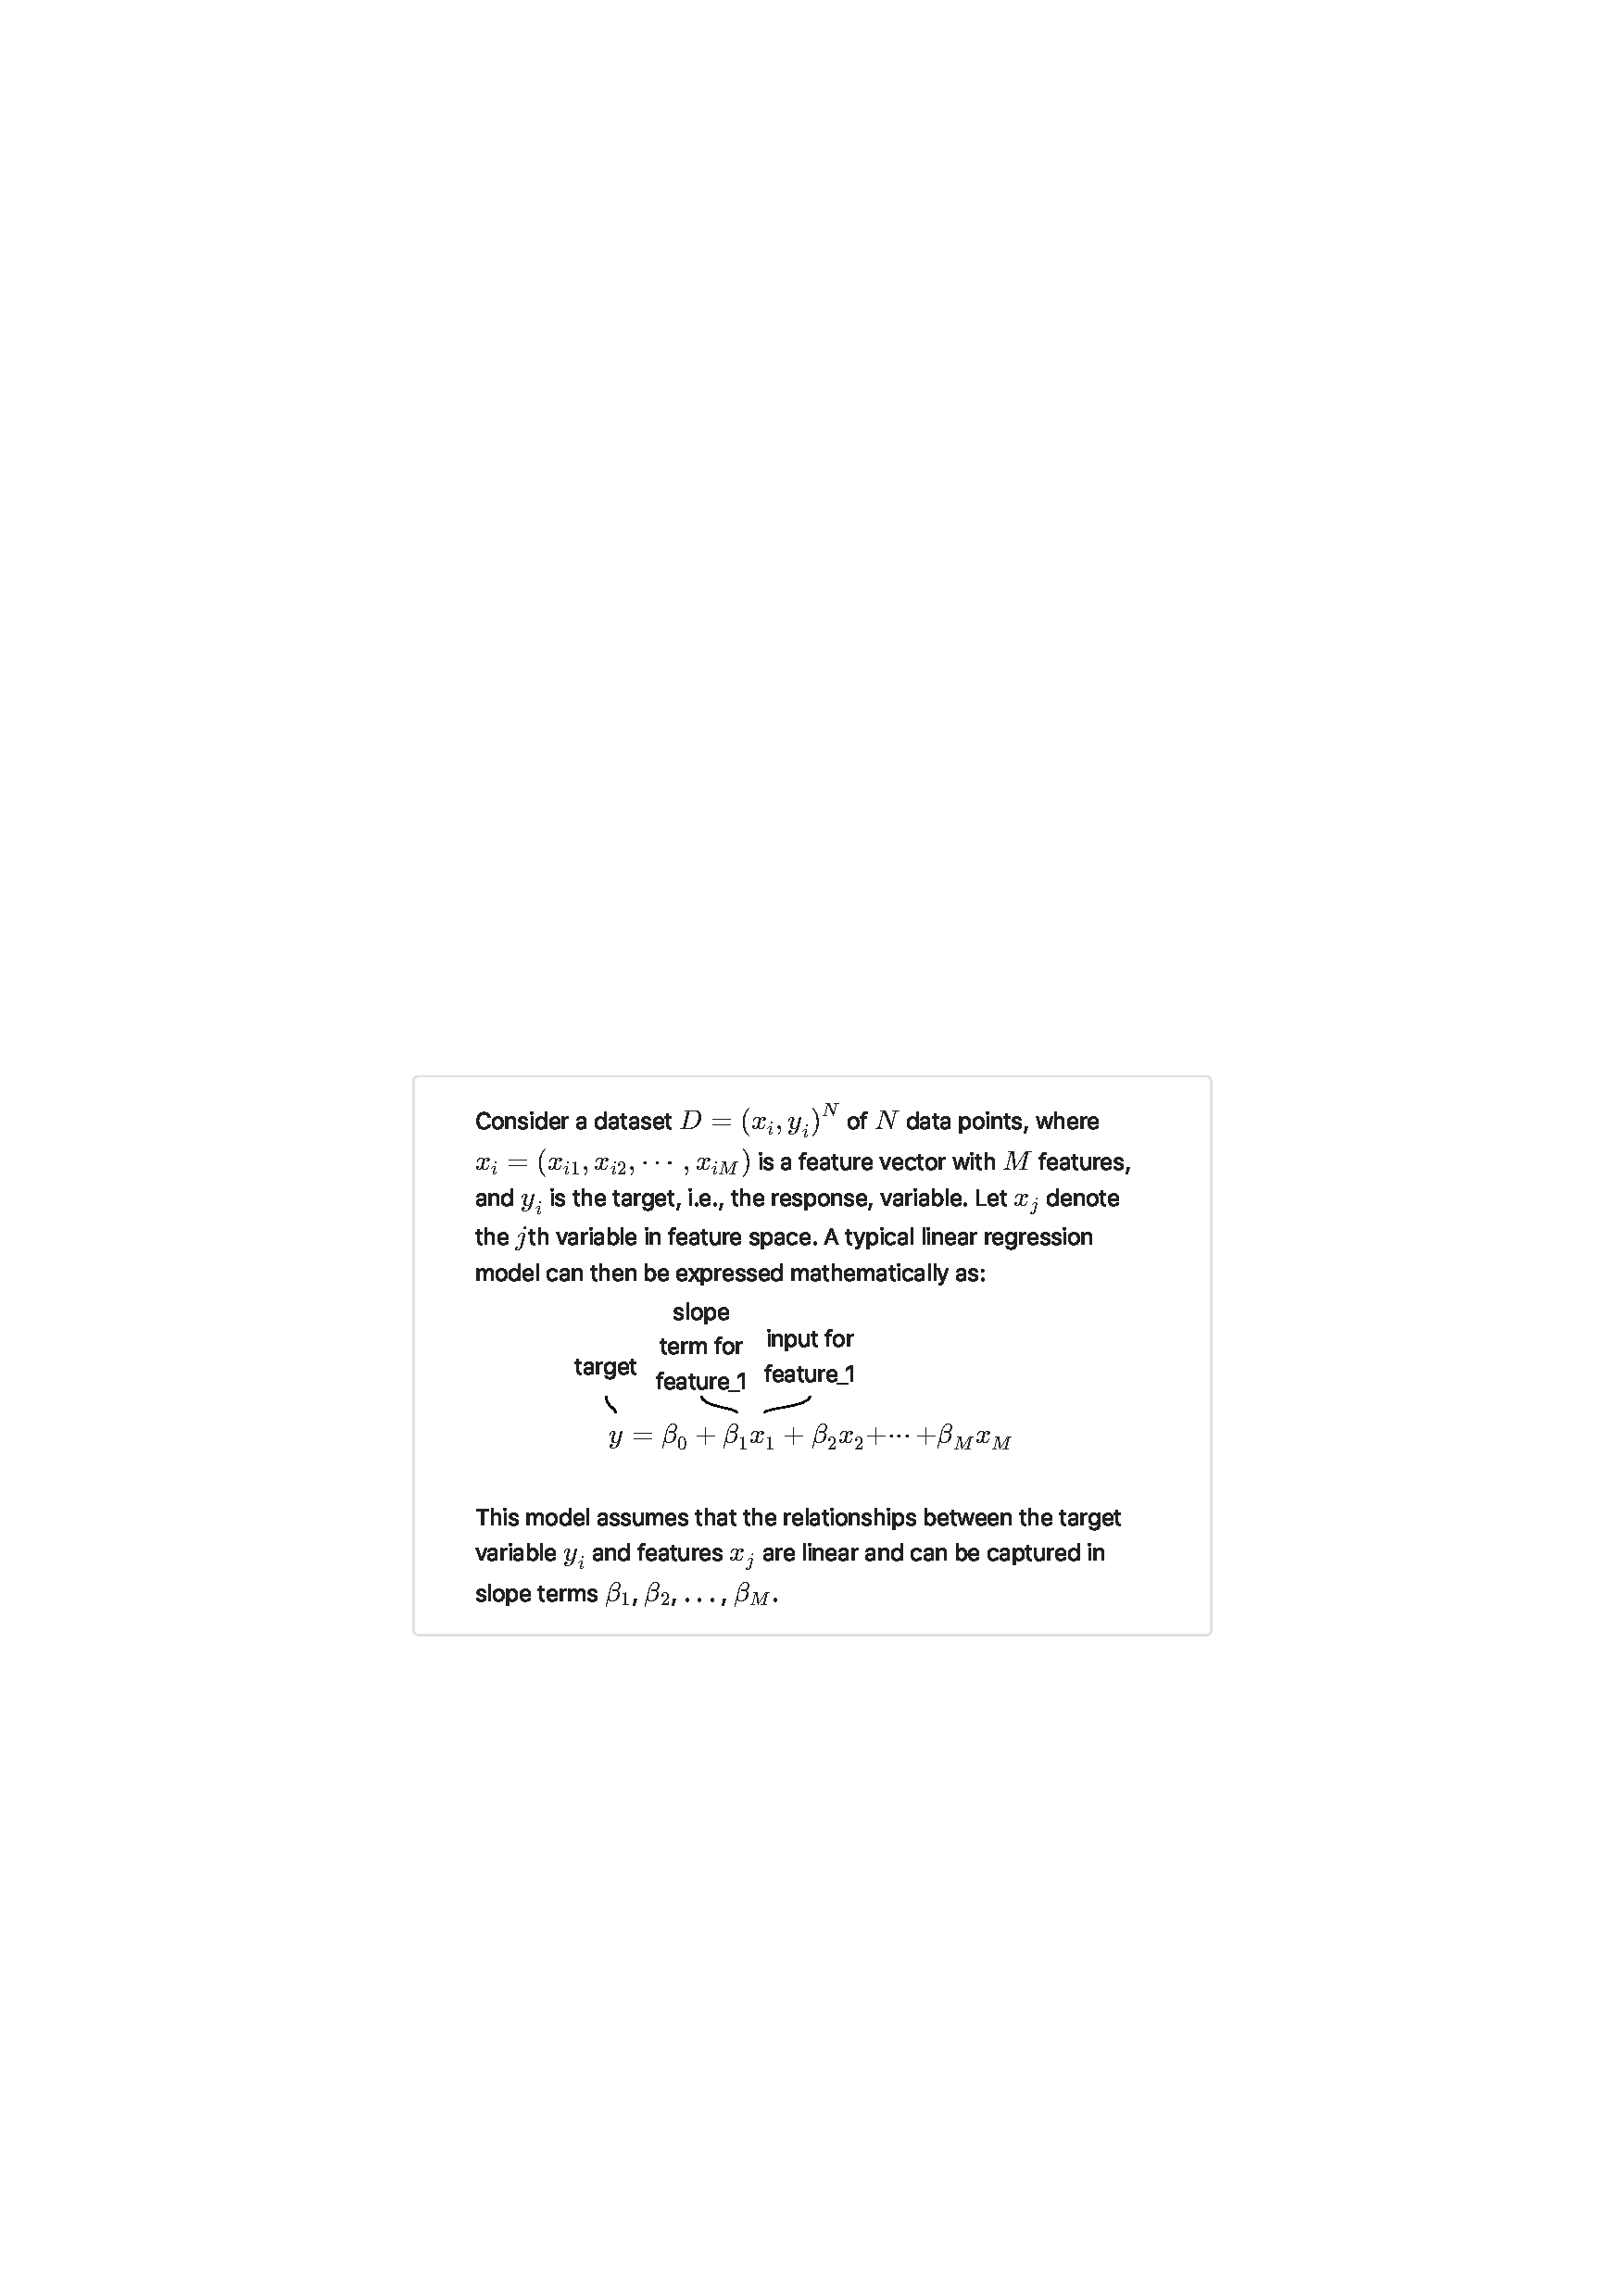
\includegraphics[width=.86\linewidth]{figures/o-3382}\Description{An example augmentation authored by P13 in the exploratory task. Only labels were used. In the block formula, “y” is labeled “target,” “beta-sub-1” is labeled “slope term for feature-underscore-1”; and “x-sub-1” is labeled  “input for feature-underscore-1.” All labels use leader lines, with labels appearing above the formula.}}

% P13 used only labels to augment the formula to improve readability for the given maths excerpt. This participant mentioned that adding labels was sufficient and concise in such a textbook-style excerpt; colors were more useful with hand-written notes.

% \begin{minipage}{\linewidth} % This minipage prevents the last image from getting split from the text on the last page
Some participants experimented more ambitiously with CSS, when they had sufficient prior knowledge. For instance, P17 experimented with \texttt{background-color}, \texttt{font-size}, and \texttt{font-weight} and expressions, in addition to the other typical augmentations.
% \\[1ex]

\centerline{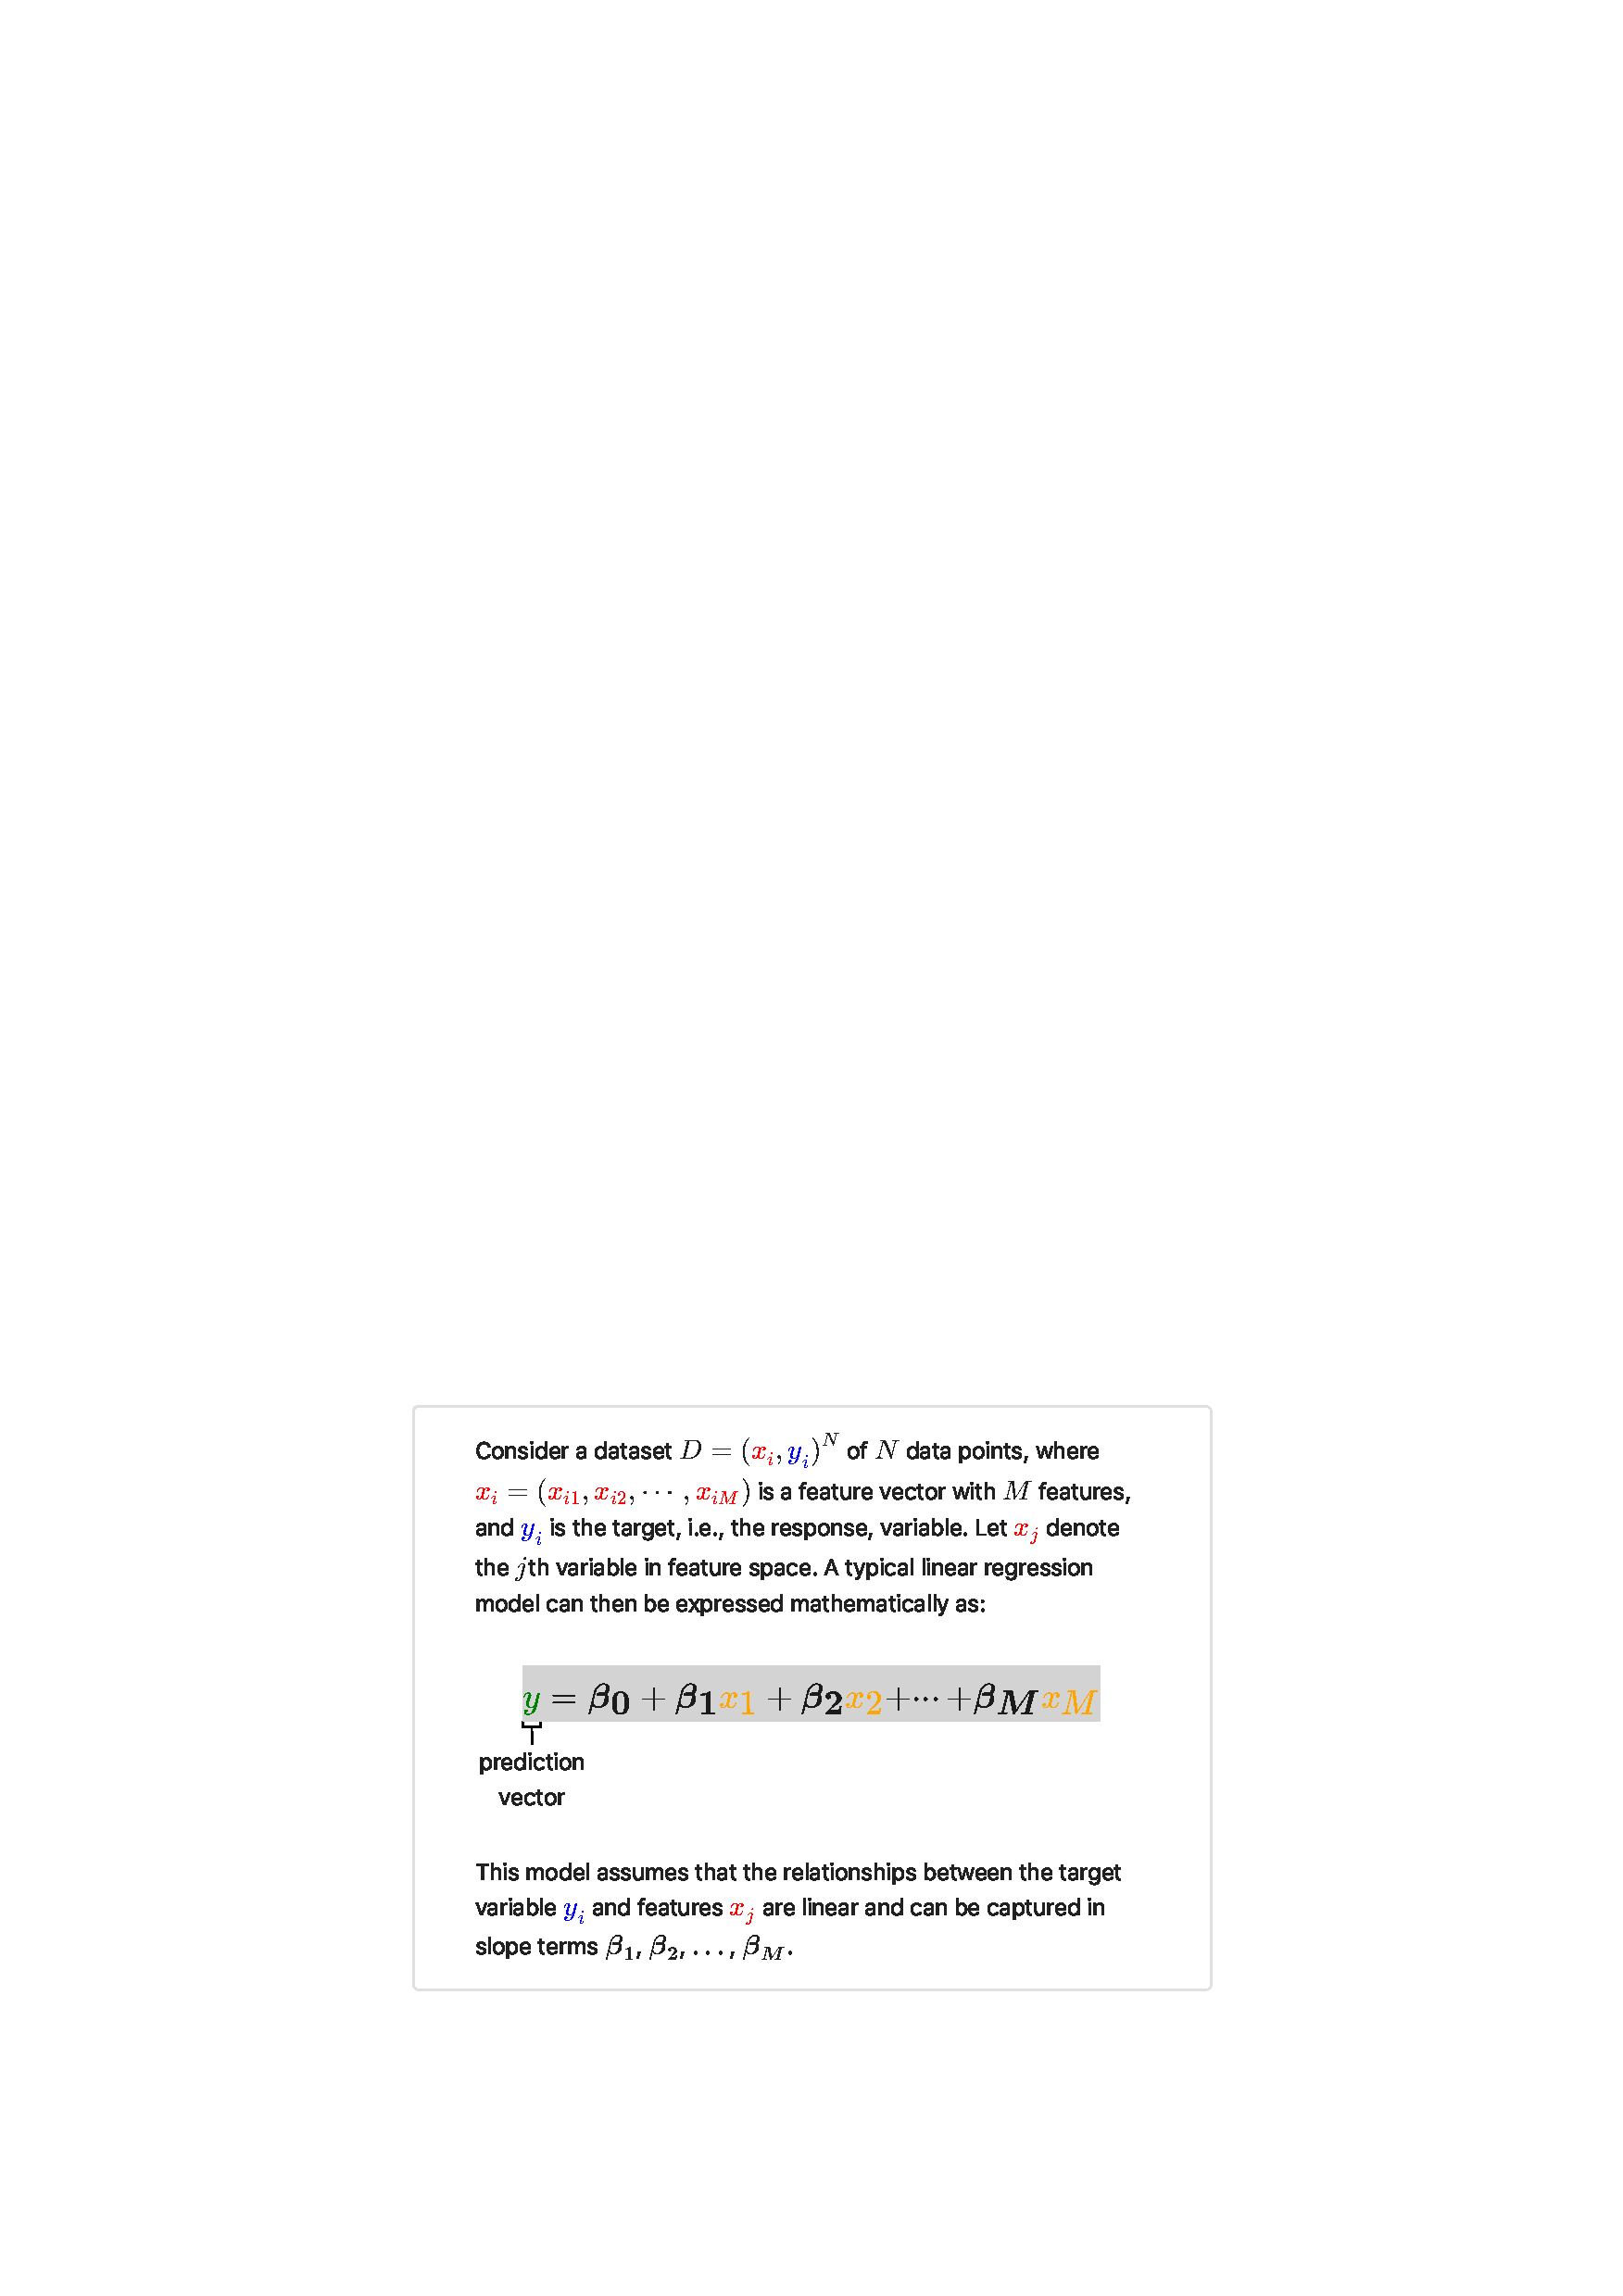
\includegraphics[width=.86\linewidth]{figures/o-3297}\Description{An example augmentation authored by P17 in the exploratory task. All symbols in the block formula are bolded and given a background color of gray. “y” is colored green and given the label “prediction vector.” Outside the formula, all “x” symbols with subscripts are colored red; in the block formula, they are given a gold color.  Outside the formula, all “y” symbols with subscripts are colored in blue. All the “beta” symbols with subscripts are bolded.}}

\vspace{-4ex}
\end{document}
